% arara: xelatex
% arara: xelatex
% arara: xelatex

% options:
% thesis=B bachelor's thesis
% thesis=M master's thesis
% czech thesis in Czech language
% english thesis in English language
% hidelinks remove colour boxes around hyperlinks

\documentclass[thesis=M,english]{FITthesis}[2012/10/20]

\usepackage[utf8]{inputenc}

\usepackage{graphicx} %graphics files inclusion
% \usepackage{subfig} %subfigures
% \usepackage{amsmath} %advanced maths
% \usepackage{amssymb} %additional math symbols

\usepackage{dirtree} %directory tree visualisation

% ADDED BY ME
%\usepackage{blindtext} % lorem ipsum
%\definecolor{mygray}{gray}{0.6}
%\newcommand{\blind}[1][1]{\textcolor{mygray}{\Blindtext[#1][1]}}

\newcommand{\blind}[1][1]{}

% ALSO ADDED BY ME
\usepackage{todonotes} 
\usepackage{multicol}

\newcommand{\todotext}[1]{\textcolor{red}{\textbf{[[#1]]}}}
\newcommand{\redtext}[1]{\textcolor{red}{[[#1]]}} 


\setlength{\fboxsep}{0.005pt}
\newcommand{\tmpframe}[1]{\fbox{#1}}
\renewcommand{\tmpframe}[1]{#1}
\newcommand{\permanentframe}[1]{\fbox{#1}}
\newcommand{\noframe}[1]{#1}


\let\myCite\cite
\renewcommand\cite{\unskip~\myCite}
\let\myRef\ref
\renewcommand\ref{\unskip~\myRef}


\newcommand\hatx{\^{}}
\newcommand{\hatxxx}{\hatx\hatx\hatx}

% list of acronyms
%\usepackage[acronym,nonumberlist,toc,numberedsection=autolabel,nomain]{glossaries}
\iflanguage{czech}{\renewcommand*{\acronymname}{Seznam pou{\v z}it{\' y}ch zkratek}}{}
%\makeglossaries

\newcommand{\tg}{\mathop{\mathrm{tg}}} %cesky tangens
\newcommand{\cotg}{\mathop{\mathrm{cotg}}} %cesky cotangens

% LB
% \setlength{\parskip}{0em}

% % % % % % % % % % % % % % % % % % % % % % % % % % % % % % % % % % % 
% % % % % % % % % % % % % % % % % % % % % % % % % % % % % % % % % % % 
\department{Department of theoretical computer science}
\title{Contextual Shell History}
\authorGN{Šimon} %author's given name/names
\authorFN{Let} %author's surname
\authorWithDegrees{Bc. Šimon Let} %author's name with academic degrees
\author{Šimon Let} %author's name without academic degrees
\supervisor{Ing. Lukáš Bařinka}

\acknowledgements{I would like to thank my supervisor Ing. Lukáš Bařinka for his guidance and advice. His insights and expertise shaped this work significantly. 

Next, my thanks go to my colleagues and friends for their valuable feedback. They helped me spot my personal biases and assumptions rooted in my personal shell workflows. 

I am grateful for the trust of hundreds of people who downloaded this project. I would also like to thank all GitHub users who submitted issues and pull requests to the project.

I want to thank Installfest conference organizers for the opportunity to give a talk and to demo this project on Installfest. 

Finally, I would like to thank my family for their support during writing this thesis and trough my whole studies.
}
\abstractCS{I dnes zůstává příkazová řádka populárním způsob jak ovládat počítač. Historie shellu umožňuje lidem snadno opakovat předchozí příkazy což zvyšuje jejich 
produktivitu.
Způsob jakým lidé používají shell závisí na kontextu jako je třeba současný adresář. V této práci chceme využít dostupný kontext ke zlepšení standartní historie shellu.

%Even nowadays, command line is a popular way to interact with computers. Shell history allows people to reuse previous commands which increases productivity. 
%The way people use shell changes based on context such as current directory. In this work, we intend to use additional context to enhance the standard shell history.

Analyzujeme funkce standartní historie a to jak je lidé používají. Identifikujeme interaktivní zpětné vyhledávání jako neefektivní mechanismus standartní historie vhodný pro náhradu. 

%We analyze standard history features and how people use them. We identify reverse search as inefficient standard feature we need to redesign.

Prozkoumáním existujících nástrojů historie shellu najdeme nástroje, které řeší problémy s interaktivním zpětným vyhledáváním. Nacházíme také kontextové nástroje historie shellu, které ale nepřináší uživateli velké zlepšení.

%By exploring existing history tools we find tools that address the issues of reverse search. We also find contextual history tools that do not bring much value to the user. 

Navrhujeme systém historie shellu, který přináší výhody existujících nekontextových nástrojů historie. Zároveň náš návrh používá kontext k dalšímu zlepšení funkcí historie shellu.

%We design a history system that matches the improvement of state-of-the-art non-contextual history tools; Plus, our design uses context to further enhance the capabilities of the shell history.

Implementujeme podstatnou část našeho návrhu. Naše řešení zaznamenává historii shellu s kontextem. Terminálová aplikace vyhledává v historii a zobrazuje relevantní výsledky na základě současného kontextu. 

%We implement a core parts of the design. It records shell history with context. A fullscreen terminal app searches the history and returns relevant results based on current context.

Na základě dát o používání od našich uživatelů porovnáváme naše řešení s populárním existujícím nástrojem pro vyhledávání v historii -- Hstr. Naše řešení v průměru podává podobný nebo lepší výkon než Hstr.

%Based on usage data from some of our users, we compare our solution with one of the state-of-the-art history tools -- Hstr.
%Our solution on average performs similarly or better than Hstr.

Existuje mnoho situací, kde naše řešení překonává Hstr. Uživatel při vyhledávání potřebuje méně znalosti a musí méně psát. Naše řešení v průměru šetří uživateli více napsaných znaků.

%We found many situations where our solution outperforms Hstr. It requires less knowledge and less typing when searching. Our solution on average saves more typed chars to the user. 

Naše řešení bylo za posledních pět měsíců nainstalováno přes 600 krát. Někteří naši uživatelé dříve používali Hstr a naše aplikace pokrývá všechny jejich předchozí potřeby. Zpětná vazba kterou jsme dostali od komunity je z velké části pozitivní.

%Our solution has been installed over 600 times in last five months. Some of our users previously used Hstr and our application covers all of their previous workflows. We have received overwhelmingly positive feedback from the community.
}

\abstractEN{Even nowadays, the command line is a popular way to interact with computers. Shell history allows people to reuse previous commands, which increases productivity. 
The way people use shell changes based on context such as current directory. In this work, we intend to use the available context to enhance the standard shell history.

% e describe target users for our system and typical workflows people perform. Based on the workflows w
We analyze standard history features and how people use them. We identify reverse search as an inefficient standard feature we need to redesign.

By exploring existing history tools, we find tools that address the issues of reverse search. We also find out that existing contextual history tools do not bring much value to the user. 
%Useful contextual history tools need to match the improvements provided by non-contextual tools.
We design a history system that matches the improvement of state-of-the-art non-contextual history tools; Plus it uses context to further enhance the capabilities of the shell history.

We implement the core parts of the design. It records shell history with context. A fullscreen terminal application searches the history and returns relevant results based on the current context.

Based on our users' usage data, we compare our solution with one of the state-of-the-art history tools -- Hstr.
Our solution, on average, performs similarly or better than Hstr.

There are many situations where our solution outperforms Hstr. It requires less knowledge and less typing when searching. Our solution, on average, saves more typed chars to the user. 

Our solution has been installed over 600 times in the last five months. Some of our users previously used Hstr, and our application covers all of their previous workflows. We have received overwhelmingly positive feedback from the community.

}
\placeForDeclarationOfAuthenticity{Prague} %where you have signed the declaration
\keywordsCS{Shell, Příkazová řádka, Historie shellu, Nástroje produktivity}
\keywordsEN{Shell, Command line, Shell history, Productivity tools}
\declarationOfAuthenticityOption{1} %select as appropriate, according to the desired license
% \website{https://github.com/curusarn/master-thesis} %optional URL (remove entirely if you have no URL for this thesis) TODO: put the thesis up

\begin{document}

%\newacronym{GUI}{GUI}{Graphical User Interface}
%\newacronym{CLI}{CLI}{Command Line Interface}
%\newacronym{GNU}{GNU}{GNU's Not Unix!}
\begin{introduction}



Classic command line interfaces were mostly replaced by GUIs in consumer software \cite{norman2007ui}. However, among IT professionals and enthusiasts, CLIs and shells are a popular way to interact with computers.\footnote{CLIs and shells are active topics on websites that are popular among developers. Specifically, GitHub Topics, Stack Overflow, and Super User all register notable activity under topics/tags about CLIs, Bash, and Zsh.} 
%CLIs are generally not replaceable by GUIs. GUIs do not work well when the number of available actions is high \cite{norman2007ui}. 

Shell history enables shell users to reuse previously entered command line submissions.
There are many people who care about shell history tools.\footnote{We have sparked a wave of reactions by asking people about what shell history tools they are using.\cite{twitter-thread}}

Shells like Bash and Zsh were initially released around the year 1990. History features in these shells have not seen many improvements since the beginning of the millennium. In this work, we analyze the standard history mechanisms to find how they could be improved.

People use shell differently in different situations. For example, some directories contain projects, and people might use different commands based on which project they are working on. We think that we could use directories and more additional information to improve the capabilities of shell history. 

We focus on Unix-based operating systems because more than half of all developers use them\footnote{According to \cite{stackoverflow2019devsurvey}, 25.6\% and 26.8\% of developers use Linux and MacOS, respectively.}. 
Default shell on GNU/Linux is Bash \cite{ramey1994gnubash} and default shell on MacOS is Zsh\footnote{According to \cite{apple2019zsh}, default shell in MacOS is Zsh since October 2019.}. Because of that, we focus on these two popular shells.

We examine standard history features and what issues people encounter when using them. We introduce target users and formulate typical shell history workflows. We explore existing history tools and how they improve standard shell history. Then, we design a new contextual history system based on our analysis. We implement the core parts of the designed system. Finally, we test the system using the data we collect from our users. Based on that, we draw conclusions about this work.

\section*{Defined terms}

\redtext{should we define the terms here?}

To avoid confusion throughout this work, we define several terms.

\begin{itemize}
    \item Command line entry $=$ the contents of the command line submitted by the user
    \item Command stub $=$ the first word of the command line entry
    \item History entry and command line submissions are sometimes used instead of command line entry.
\end{itemize}

\end{introduction}

% \begin{verbatim}
% ____5___10___15___20___25___30___35___40___45___50___55___60__64
% \end{verbatim}
% The page is 64 verbatim characters wide


\chapter{Analysis}

In this chapter, we look at the current state-of-the-art. 
We examine standard shell features because they represent both what people are used to and the starting point for our solution.

Because we want to know who we design for we introduce target users for our future design. We formulate shell history workflows based on shell usage data we have collected from several people. %Each workflow is described in detail. 
These workflows show us when standard shell history features work well and when there are issues. We explain the limitations and disadvantages of standard shell history features.

After that, we review existing history tools to see what problems they solve. We identify tools that address the issues of standard shell history features. We also find contextual history tools that do not bring much value to the user.

Then, we explore what contextual information is available in shell. We break it down into multiple distinct categories. For each category, we describe how it relates to shell usage and how it could be useful in history tools.


\section{Standard shell history features}

In this section, we describe common standard shell history features of Bash\cite{bashman} and Zsh\cite{zshdocs}. Most of these features are enabled by default; The user can use them without configuring them first.
We cover following history features:

%For each of the features, we point out its advantages and disadvantages.
%The list of history features we cover the following:

\begin{itemize}
    \item Saving history entries
    \item History substitution
    \item Stepping through recent history
    \item Prefix search
    \item Reverse search
    \item Manual history filtering
\end{itemize}


\subsection{Saving history entries}

%First, we take a look at how command line entries are saved into history.
Whenever you submit a command line entry in shell, it is added to the history. Saved history entries are then available for future reuse. %We describe specific ways to access the history a bit later.

It is possible to configure shell to not save duplicate entries to history. 
In Zsh, we can also keep duplicates in history but prevent them from showing up when searching. 
There are options to prevent specific command line entries from being saved to history based on a user-specified pattern. %This is done using \verb|HISTIGNORE| option in Bash.

We can configure shell history to save the time of the execution alongside the history entry. In Zsh, it is also possible to record and save the duration of the execution.

\paragraph{Missing history entries}

When we execute a command line entry, we generally expect to be able to find it in history. This is not always the case. There are multiple reasons why executed command line entries can be missing in the shell history.

In Bash, simultaneous terminal sessions can overwrite the history of one another when it is being written to disk.\cite{bashman}\cite{bash-session-issues-1} This can be prevented by properly configuring the shell.

Shell history is not unlimited. We might not be able to find history entries simply because they are too old and our history size is too small. The size of shell history can be increased with configuration options. % \verb|HISTSIZE| and \verb|SAVEHIST| or \verb|HISTFILESIZE|.

\subsection{History substitution}

History substitution is a powerful feature that allows users to reuse previous history entries or their parts. 
For example, we can use \verb|!!| to repeat previous history entry and \verb|!$| to repeat its last argument. Executing a history entry based on its absolute or relative index can be done using \verb|!5| or \verb|!-2|, respectively.

The flexible notation of history substitution makes it possible to match recent history and perform substitutions on them. For instance, \verb|!cc| executes the last history entry that starts with \verb|cc|. An example of substitution is \verb|!!:s/foo/bar/|. It retrieves the previous history entry and replaces instances of \verb|foo| with \verb|bar|.

History substitution is powerful and flexible, but it is non-interactive. Users do not know what the substitution evaluates to until they execute it. For example, submitting \verb|!rm| could lead to irreversible losses.

It is possible to configure shell to show us the result of the substitution before executing it. Doing so, however, adds an extra step to each history substitution we perform. The additional required interaction can be very annoying in simple cases such as \verb|sudo !!|. A less invasive way to evaluate the substitutions before execution is \verb|magic-space|; It causes shell to expand substitutions after we press \verb|SPACE|.

\subsection{Stepping through recent history}

Repeatedly pressing \verb|ARROW_UP| gives us access to immediately previous history entries. Conversely, we can press \verb|ARROW_DOWN| to get back to the original command line. 

This is a quick and convenient way to access recent history entries. Instead of trying to remember the previous history entries, we can interactively step through them.

Quite obviously, this is not a great way to access older than recent history entries. Pressing \verb|ARROW_UP| many times and reading the results as they appear can take considerable amounts of time.

\subsection{Prefix search}

Prefix search works similarly as stepping through history using \verb|ARROW_UP|. It returns previous history entries that match the prefix we have already typed. 
This enables us to reuse recent and even older history entries based on their prefix. Prefix search is convenient in practice. For example, we can search for the previous \verb|git| commands which all most likely start with \verb|git| prefix.

When there is no prefix, prefix search works just like simple stepping through recent history. Because of that, it can be bound to arrow keys and used as a reasonable replacement for the default behavior. We can find prefix search configured this way in a popular Zsh configuration framework -- Oh-my-zsh\cite{toolsohmyzsh}.

In both Bash and Zsh, the prefix search is not configured by default. Before we people can start using it, they need to find out that it exists and configure it. This is one of many examples where we can see the importance of default configuration. Many people only know the default state of the shell because they never change the default configuration.

\subsection{Reverse search}

With the prefix search, we could only search the history by a prefix.
Reverse search allows us to interactively search for previous history entries based on any part of the command line entry. It can be activated using \verb|CTRL-R|.

In contrast to prefix search, the reverse search is available by default, and people seem to use it a lot. Reverse search is the most powerful interactive history search feature included in Bash and Zsh.

The reverse search might seem like the perfect way to search history. However, it does have its limitations. First, we cannot search using more than one word. In other words, the search query needs to be consecutive. Second, only one result is displayed at a time. We need to repeatedly press \verb|CTRL-R| to see more results.

Pointing out these limitations might seem like nitpicking. However, later we will see that they do limit the searching capabilities of reverse search significantly.


\subsection{Manual history filtering}

Shells offer built-in commands to print and control history. Built-in command \verb|history| and standard shell utilities can be used for powerful history searching.
For example, to search the history using two words and displays all matching results we can run following command line entry. 
\begin{verbatim}
    history | grep 'word1' | grep 'word2'
\end{verbatim}

Manually filtering history overcomes the limitations of reverse search. However, extra typing is necessary to complete the searches compared to interactive methods. Plus, unlike with reverse search, we cannot see the results update as we type the search query.


\section{Target users}

When designing any product, we need to make sure we know who the product is for. Shell history tools are no exception. To capture the target user-base, we are modeling two typical users as personas.

% As the first persona, we chose an experienced user because shell history tools are likely more for users that use shell extensively. As the second persona, we chose a novice shell user; Designing tools for novice shell users can result in a product that is better for everyone. For example, it is especially important for novice users that the product is easy to install, comes with a good default configuration, and is easy to use for the first time; These characteristics are beneficial to everyone not just novice users. 

\subsection{Typical experienced shell user}

Experienced professional programmer \textit{Peter} develops, deploys, and operates back-end applications. The main languages he uses at work are C and C++. He has years of experience with developing on and for the Linux operating system. He is proficient in Bash, and he has written a few small shell scripts to increase his productivity.

His editor of choice is Vim. He has a sizable Vim configuration with multiple Vim plugins he collected over the years.

The shell he uses is Zsh with Oh-my-zsh \cite{toolsohmyzsh} shell configuration framework. On top of that, he maintains a set of his own custom options and aliases. He puts the resulting configurations on his machines. He does not change his configuration often, but he likes to be able to configure his shell and other tools he uses.

He often uses \verb|ssh| to log into remote machines. The remote machines are shared and have the default shell configuration. He keeps his shell and editor configuration somewhat similar to the default one because he does not want to constantly switch between very different environments. 

His daily shell workflows include complex commands with many long arguments and switching between many different projects. When coming back to a project, he sometimes cannot remember what command line entries he was using. He is familiar with Make, but he often forgets to create Makefiles for typical tasks in projects.

He makes use of interactive history features like reverse search and prefix search. However, he quite often uses manual history filtering.

\begin{verbatim}
    history | grep 'pattern1' | grep 'pattern2'     
\end{verbatim}

It is more powerful than the reverse search and sometimes it also feels more comfortable. Manual filtering allows him to search by more than one pattern and to see many of the matching results. 

\subsection{Typical novice shell user}

Junior data analyst \textit{Mark} has recently started his first job. He uses shell because he needs it at work. The primary language he uses is Python. 

The editor he uses is Visual Studio Code because it was recommended to him by a coworker. He likes that it suggests extensions to install based on files he is working with.

He is using Bash with the default configuration provided by Ubuntu distribution. Apart from that, he does not have any custom shell configuration. 

Since he does not have much experience with shells, he does not understands the shell configuration files. Because of that, he does not feel confident editing them. 

If he discovered or someone recommended a new shell tool to him, he would prefer an installation without the need to edit the shell configuration files. Additionally, he expects any programs and tools he installs to work out-of-the-box without requiring much configuration. 

There are shell history features he is not aware of such as history substitution and prefix search. He uses arrow keys to get recently submitted command line entries, and he presses \verb|CTRL-R| when looking for history entries further in the past. 


\section{Common shell history workflows}

Now that we know who our target users are, we can formulate common workflows for them. Workflows are formulated based on interviewing users, collected shell usage data\footnote{We have collected shell history and usage data from a few people with different experience levels. We used this data to find workflows and to determine how common different workflows are.}, and our experience with shells. 

Some of the workflows can be easily fulfilled using standard history features. Others are either difficult or impossible to complete. We describe and explain the issues people can encounter when using standard history features. 

\newpage
In the next few sections, we describe following workflows in detail:


\begin{itemize}
    \item Editing an immediately preceding history entry
    \item Blindly retrieving very recent history entries
    \item Retrieving recent history entries
    \item Editing retrieved history entries
    \item Repeating a sequence of history entries
    \item Searching with limited knowledge
    \item Searching with implicit context
\end{itemize}


\subsection{Editing an immediately preceding history entry}

In this first workflow, the user submits a command line entry but is not satisfied with the result. To fix that, he retrieves the immediately preceding history entry, modifies it, and executes it again. We will look at multiple example sequences of command line submissions for this workflow.

\begin{verbatim}
    wget https://pastebin.com/raw/EDELXNYp --silent
    wget https://pastebin.com/raw/EDELXNYp --quiet
\end{verbatim}
In this example, the user is trying to download a file from \verb|pastebin| using \verb|wget|. The first command ends with a non-zero exit status because \verb|--silent| is not an option of \verb|wget|. He presses \verb|ARROW_UP| to retrieve the previous command line entry, fixes the mistake, and presses \verb|ENTER| to submit the command line entry again. 

Using \verb|ARROW_UP| is efficient in situations when we need to either edit the end of the command line entry or append to it.
The next example shows a different case.

\begin{verbatim}
    apt-get install zsh
    sudo !!
\end{verbatim}

Here, the user wants to install the \verb|zsh| package. The command fails because superuser permissions are needed to install packages to the system. Instead of using interactive history features, the user uses history substitution \verb|!!| which repeats the previous history entry. 

By using \verb|!!| we can efficiently prepend or append to the previous command line entry. There are other history substitutions but \verb|!!| is by far the most commonly used one. 

So far, we only saw situations where the submitted command line ended with a non-zero exit status, and then the user fixed the error. This is not always the case because not all errors result in a non-zero exit code. Some errors are logical, and not all programs respect the convention of properly signaling errors. Additionally, users sometimes gradually change and develop a command line entry to make sure that each step of the process works as intended. This is shown in the example below.

\begin{verbatim}
    sort data.txt
    sort data.txt | uniq -c
    sort data.txt | uniq -c > data_processed.txt
\end{verbatim}

In this next example, we see how the user processes \verb|data.txt| file. In each step, he uses \verb|ARROW_UP| to retrieve the previous history entry and continues editing it. When he is satisfied with the result, he redirects the processed data into a file. 

This example shows that there is not always an explicit error that could be detected by the shell to predict that the user will retrieve the previous history entry. It also shows that the editing process can often be continuous.

We just saw multiple different situations in which people continue working on the same command. We also saw different approaches to retrieving previous history entries. It is worth noting that in all of these situations, the user relies on the order of the shell history. 

\subsection{Blindly retrieving very recent history entries}\label{workflow-blind-retrieval}

This second workflow is a retrieval and execution of a very recent history entry. Here, the user remembers the exact position of the history entry he wants to retrieve. An example of such workflow is running the following sequence of command line submissions.
\begin{verbatim}
    make build
    vim hello_world.c
    make build
\end{verbatim}
First, we use \verb|make| to build a project. Then we edit a file using \verb|vim|. After that, we press \verb|ARROW_UP| twice and press \verb|ENTER| to execute the retrieved history entry -- \verb|make build|. 


Consider, if we used a graphical editor or if we ran the editor from a different terminal. In such case, we would only have to press \verb|ARROW_UP| once but the workflow would essentially stay the same.

When retrieving very recent history entries the users often remember the exact position of the history entry; This means that they do not read the history entry that appears on the command line but they blindly execute it instead. This is an efficient workflow that shows us the importance of the order of recent history entries.

\subsection{Retrieving recent history entries}\label{workflow-recent-history-arrow-up}
The third workflow is a retrieval of history entry that is still recent, but the user no longer remembers the exact position in the history list. This means that the user needs to read the history entries as they appear to see if the desired entry was retrieved. An example sequence of command line entries for this workflow follows.

\begin{verbatim}
    systemctl start nginx.service
    systemctl status nginx.service
    tail /var/log/nginx/error.log
    nginx -t
    vim /etc/nginx/nginx.conf
    nginx -t
    systemctl start nginx.service
\end{verbatim}

In this example, the user is trying to start an Nginx \cite{reese2008nginx} web server. At first, the server does not start, and the command returns an error. The user quickly realizes that there is a syntactic error in the configuration file after checking it using \verb|nginx -t|. Then, the configuration is fixed using \verb|vim|, and the syntax is rechecked using \verb|nginx -t|. 

At this point, the user presses \verb|ARROW_UP| five or six times\footnote{It could take five or six depending on whether or not the user has history deduplication turned on.} to retrieve a recently executed command line entry \verb|systemctl start nginx.service|. Every time they press \verb|ARROW_UP| a single result appears, and they need to read it. There is no way to tell if the desired result is one press of a button away, three, or seven. % When the user presses \verb|ARROW_UP| too many times, they can show previous history entries by pressing \verb|ARROW_DOWN|.


% It seems that people experience the sunk cost fallacy\footnote{\redtext{TODO: describe?}} which combined with the lack of feedback from the system drives them to stick to the original plan -- pressing \verb|ARROW_UP|. 

You might think that people would not press \verb|ARROW_UP| five or six times and would rather use other history mechanisms.
However, the usage data we collected shows that even someone who claimed not to press \verb|ARROW_UP | excessively actually does so quite often. Pressing \verb|ARROW_UP| five times is more common than you would expect, and pressing it over ten times is rare, but it still happens. We also quite often saw people pressing \verb|ARROW_UP| too many times and then using \verb|ARROW_DOWN| to go back to previous history entries. We think that it is easy to overshoot when you only see one history entry at a time.

%\todo{we could include reasons why people do this but I don't think it's necessary/important (see drafts in comments)}

% 1-2 was the most common ... 5-6 quite common ... 8 - 10 rare 20 exceptions
% WHY: sunk cost fallacy + lack of feedback from the system
% WHY: people might not realize how far the entry is in the first place
% WHY: people do not want to "abandon the effort they have already put in" because anytime the result could be there

%It seems that in situations like this one people do remember the history entry well and perceive it as recent. This is why they chose to use 

\paragraph{Prefix search}

An efficient alternative way to fulfill the same workflow is to use the prefix search. To use prefix search, the user needs to remember the first word or at least the first few characters of the command line entry; This is likely since all the command line entries we are retrieving in this workflow are recent.

We will use the example with Nginx to compare using prefix search with the simple stepping through recent history. When using prefix search, the user types in a prefix -- \verb|systemctl| -- and presses \verb|ARROW_UP| twice to get to the desired history entry. In contrast, when only using \verb|ARROW_UP|, it took five or six presses to get to the history entry.

This might not seem like an improvement because we need to type the prefix before we start pressing \verb|ARROW_UP|. However, we have to realize that going through multiple history entries and reading them one by one requires a significant amount of time and effort compared to typing. 
This is a good example of how the number of keystrokes is not the only thing we should be taking into account. Generally speaking, shell history should save effort and time of its users. Retrieving previous history entries should be both mechanically and cognitively less demanding than typing them again.\cite{greenberg1993computer}

% REF(greenberg): Recurring inputs should be reentered more easily than the user's original entry, with the aim of reducing both physical tedium and the cognitive overhead of remembering past inputs. Reuse facilities should not be targeted only to experts, as they can help everyone.

% the prefix could be shorter e.g. "sys", "system" ... typing vs. effort required to decide how long/short prefix is sufficient

%\todotext{Is this ending good? - continue (check comments)}

% ADD(polished?): There is a vocal group of people with strong preference for prefix search. The rest of the people either do not know that prefix search exists, do not have it configured, or prefer plain \verb|ARROW_UP| possibly out of habit.
% NOTE: maybe this^ belongs earlier? (but maybe not)


\subsection{Editing retrieved history entries}

In the previous section, we saw a workflow where the user retrieved a recent history entry and executed it without any changes. Now, we look at a similar workflow. Here, the user retrieves a history entry, edits it, and then executes it again. Workflows with editing are a little less common than those with direct execution according to the usage data we collected. An example of a workflow with editing follows.

\begin{verbatim}
    curl --data "value=test" http://localhost:8080/submit
    git add pkg/submit/submit.go
    git commit --message "fix submit endpoint"
    git tag v2.4.0-rc.1
    git push
    git push --tags
    curl --data "value=test" http://test.example.com:8080/submit
\end{verbatim}


Here, the user is using \verb|curl| to test a server endpoint running locally at \verb|localhost:3000/submit|. After being done with the testing, he commits the changes, tags the version as a pre-release\footnote{Here "rc" in "v2.4.0-rc.1" version stands for release candidate which is sometimes used to mark pre-release versions.}, and pushes both commits and tags to the upstream. This triggers a CI pipeline that deploys the new version to the testing environment. The user wants to test that the endpoint also works there.

At this point, the user presses \verb|ARROW_UP| six times to get to the desired history entry.\footnote{Alternatively, he could also use prefix search which would be more efficient.} 
After retrieving the desired history entry, the user needs to edit it to change the server URL from \verb|localhost| to \verb|test.example.com|. He holds down \verb|ARROW_LEFT| for about a second, holds down \verb|DELETE| for about a second, types \verb|test.example.com|, and finally executes the changed command line entry. 

This seems a little tedious, but it is still more efficient than typing the whole command line entry from scratch. Instead of navigating by and deleting single characters, we could use \verb|CTRL+ARROW_LEFT| to navigate by words and \verb|ALT+BACKSPACE| to delete whole words; This would be faster and more efficient. %However, it seems that many people do not use the command line editing functions.\todo{TODO: Ask more people, so far more people use it than I expected}

This workflow shows us how people edit history entries after they retrieve them. We see that standard history mechanisms make it possible to edit history entries after retrieval. %Reverse search, which we did not see in any workflow yet, is not an exception. 
This is a useful property that we should include in our designs as well. 

\subsection{Repeating a sequence of history entries}\label{workflow-repeating-a-sequence}

In this workflow, the user has executed a sequence of command line entries. He wants to retrieve and repeat all the command line entries in the sequence. 
Consider the following example.

\begin{verbatim}
    gcc generate_dot.c -o generate_dot.out
    ./generate_dot.out > graph.dot
    dot -Tpng -ograph.png graph.dot
    feh graph.png
    gcc generate_dot.c -o generate_dot.out
    ./generate_dot.out > graph.dot
    dot -Tpng -ograph.png graph.dot
    feh graph.png
\end{verbatim}

In this example, we are editing the \verb|generate_dot.c| file in another window. In current terminal, we compile a source file \verb|generate_dot.c|, generate a graph in the DOT\cite{graphvizthedotlanguage} language, run Graphviz\cite{ellson2001graphviz} command \verb|dot| to generate an image, and finally use image viewer \verb|feh|\cite{toolsfeh} to display the resulting image.

% ALT (too long): After observing the resulting image, we edit the source file \verb|generate_dot.c| in another window.
After observing the image, we edit the source file \verb|generate_dot.c| in another window.


Now, we want to repeat the whole process of generating the graph and view the resulting image. To retrieve the \verb|gcc| history entry, we press \verb|ARROW_UP| four times. Retrieving the next \verb|./generate_dot.out| entry also takes four presses of \verb|ARROW_UP|. Similarly, we need four keypresses for each of \verb|dot| and \verb|feh| history entries. 

We need four keypresses every time because with each executed command line entry, we are pushing all the history entries further back in the history. We see that using \verb|ARROW_UP| to repeat a block of history entries is quite inefficient. 

There is another standard history mechanism we could use to repeat a block of history entries. 
Executing \verb|fc -4 -1| opens an editor with the last four history entries and then, closing the editor executes the commands. This, however, is quite cumbersome in practice, and not many people seem to use it. 


Repeating a sequence of history entries is not the most common workflow. However, it shows us the limits and inefficiencies of standard shell history.


\subsection{Searching with limited knowledge}\label{workflow-search-w-limited-knowledge}

In all the workflows we discussed so far, the user wanted to retrieve a fairly recent history entry. Now, we move on to workflows where the user searches for older history entries. In these workflows, the user's memory is often a limiting factor; Both the knowledge of shell history and the desired command line entry are limited.

Below, we see an example of such workflow. The upper part contains relevant history entries from history. In the bottom part, we see the command line entry the user wants to find. 

%This means that simply pressing \verb|ARROW_UP| is no longer an effective way to retrieve them.
% \redtext{We are going to look at multiple examples of workflow where the user searches for an older. We will discuss how the workflow changes when the user remembers less and less information about the desired history entry. The first example follows.}


\begin{verbatim}
# relevant history entries:
    cd git/thumbnail_api
    ssh root@thumbnail-api.dev.example.com
    scp root@thumbnail-api.dev.example.com:/log/thumbnail/1.log
    git commit -m "improve api logging"
    ...
    cd git/thumbnail_worker
    ssh root@thumbnail-worker-1.dev.example.com
    ssh root@thumbnail-worker-2.dev.example.com
    ssh root@thumbnail-worker-3.dev.example.com
    ...
    ssh 192.168.2.105
# desired command line entry:
ssh root@thumbnail-api.dev.example.com
\end{verbatim}

In the example above, the user wants to remotely log into a \verb|thumbnail api| server in the development environment using \verb|ssh|. 

If the user saw the full example in front of him as we do now, it would be quite easy to choose a good searching strategy. However, the user does not see, nor he remembers all the relevant information. He will need to make use of his limited memory to find the desired command line entry. 

A common way to search shell history is reverse search. The user initiates the reverse search by pressing \verb|CTRL-R| and types in the query \verb|thumbnail|. The resulting prompt is shown below.\footnote{The search result and the prompt should be on the same line. We moved them to separate lines because they would not fit the page otherwise.}
% Reverse search displays a single most recent history entry that matches the query 

\begin{verbatim}
(reverse-i-search)`thumbnail': 
    ssh root@thumbnail-worker-3.dev.example.com
\end{verbatim}

Here, we see that the \verb|thumbnail| query matched a history entry that is not very relevant. The user makes the query more specific by typing \verb|-api|.

\begin{verbatim}
(reverse-i-search)`thumbnail-api': 
    scp root@thumbnail-api.dev.example.com:/log/thumbnail/1.log
\end{verbatim}

The reverse search still does not show the desired history entry. However, it shows a result that is much closer to what the user is looking for. The user thinks that the query is specific enough and presses \verb|CTRL-R| to show the next search result.

\begin{verbatim}
(reverse-i-search)`thumbnail-api':
    ssh root@thumbnail-api.dev.example.com
\end{verbatim}

The next result is the desired history entry; The user can press \verb|ENTER| to execute it. This was a pretty efficient but also a quite idealistic reverse search example. It worked out so well because the user was able to provide a specific enough query -- \verb|thumbnail-api|. We should look at a more realistic situation where the user struggles to come up with such a query. 

\paragraph{Realistic example of reverse search}

In this example, we are using the same shell history and desired command line entry as in the previous example. Again, the user wants to remotely log in to a \verb|thumbnail api| server in the development environment using \verb|ssh|. He presses \verb|CTRL-R| and starts searching using \verb|ssh| as a query; It is very natural and quite common to use the beginning of the line as a query in reverse search.

\begin{verbatim}
(reverse-i-search)`ssh': ssh 192.168.2.105
\end{verbatim}

The most recent matched history entry does not look very promising. The user tries to extend the query to \verb|ssh thumbnail|.

\begin{verbatim}
(failed reverse-i-search)`ssh thumbnail': ssh 192.168.2.105
\end{verbatim}

Here, we see how the user struggles to make the query more specific; Extending the query requires knowledge of the details of the desired command line entry. The user does not remember that he should be logging in under \verb|root|. % It is exactly details like this one that we hope to retrieve from shell history so that we do not need to remember them. 

The user sees that the search has failed, and so he aborts it by pressing \verb|CTRL-C|. Then, he starts over by pressing \verb|CTRL-R|. He types \verb|thumbnail| as a query, hoping it will bring better results.


\begin{verbatim}
(reverse-i-search)`thumbnail':
    ssh root@thumbnail-worker-3.dev.example.com
\end{verbatim}

This result is an improvement over the previous one. However, it is still far from what we are looking for. The user should extend the query to make it more specific. 

Previously, we assumed that the user remembers enough to extend the query to \verb|thumbnail-api|; That is a bold assumption. What if the user does not remember that words \verb|thumbnail| and \verb|api| are adjacent or that they are delimited by a dash symbol? In practice, it is hard to come up with a query that only matches the desired history entry. Oftentimes, the query matches many other history entries, which forces us to go through multiple search results.


The user is in a similar situation. He presses \verb|CTRL-R| repeatedly to display the search results one by one. At first, the user presses \verb|CTRL-R| slowly to have enough time to read the results. After about three keypresses, he becomes impatient and speeds up. This does not leave enough time to properly read each of the results, which causes him to press \verb|CTRL-R| one too many times.

\begin{verbatim}
(reverse-i-search)`thumbnail': cd git/thumbnail_api
\end{verbatim}

The user knows that pressing \verb|CTRL-S| should bring back the previous result. However, he also knows that pressing \verb|CTRL-S| freezes all input coming to his terminal; This is the default\footnote{In default configuration on many popular distributions CTRL-S produces XOFF -- a software flow control sequence that stops all input coming to the terminal.} behaviour and he could never be bothered to find out how to fix it.

At this point, the user gets annoyed because the only option is to start over. He aborts the search, presses \verb|CTRL-R|, and types in the query \verb|thumbnail|. Then, it takes five presses of \verb|CTRL-R| to get to the desired result; This time he is more careful not to go too far again.


\paragraph{Limits of reverse search}

As we just saw, the reverse search is not always an effective way to search the shell history. It heavily relies on the ability of the user to form a single continuous query; A single query that is specific enough to match the desired history entry without matching many other history entries. 

This drawback is further amplified by only displaying a single result at a time. Showing multiple results at a time would make it easier to find the desired history entry in cases when there are many matching results. 

Despite these downsides, the reverse search is a quite popular way to search the shell history. Why do people use it, given the disadvantages we discussed? The reverse search is not without its flaws, but it is still the most powerful interactive way to search the shell history. %We suspect that many people simply use what is available by default.

If the reverse search is as bad as we claim, are there other alternatives that people choose to use instead? Another quite popular method people use is manual history filtering. Manual filtering searches the history non-interactively; It brings its own set of advantages and disadvantages, which we cover in the next section.


\paragraph{Manual history filtering}

As mentioned before, manual filtering is a popular non-interactive way to search the shell history. It can be used to fulfill similar workflows as the reverse search. To properly compare the two methods, we will use the same example as before. You can see the same relevant history entries with the same desired history entry below.


\begin{verbatim}
# relevant history entries:
    cd git/thumbnail_api
    ssh root@thumbnail-api.dev.example.com
    scp root@thumbnail-api.dev.example.com:/log/thumbnail/1.log
    git commit -m "improve api logging"
    ...
    cd git/thumbnail_worker
    ssh root@thumbnail-worker-1.dev.example.com
    ssh root@thumbnail-worker-2.dev.example.com
    ssh root@thumbnail-worker-3.dev.example.com
    ...
    ssh 192.168.2.105
# desired command line entry:
ssh root@thumbnail-api.dev.example.com
\end{verbatim}

As in the previous example, the user wants to remotely log in to the \verb|thumbnail| \verb|api| server in the development environment using \verb|ssh|. He uses the \verb|history| built-in to print the shell history together with the \verb|grep| command to filter the history entries.

First, he types \verb#history | grep ssh#; The output could look something like this.

\begin{verbatim}
$ history | grep ssh
...    ...
421    ssh root@thumbnail-api.dev.example.com
450    ssh root@thumbnail-worker-1.dev.example.com
451    ssh root@thumbnail-worker-2.dev.example.com
452    ssh root@thumbnail-worker-3.dev.example.com
489    ssh 192.168.2.105
\end{verbatim}


Using manual filtering displays all five matching history entries at the same time. The user can skim through the results looking for the desired history entry. 
After he finds the result, he can either copy and paste it using a mouse or can use history substitution.

The user found the desired history in the list and uses history expansion to execute it. He types \verb|!421| and presses \verb|ENTER|.

\begin{verbatim}
$ !421
    ssh root@thumbnail-api.dev.example.com
\end{verbatim}

This was pretty quick and efficient. However, what if there were more matching history entries? What if the user could not spot the desired history entry in the list of results?

In such a case, nothing prevents the user from further filtering the results. Pressing \verb|ARROW_UP| retrieves the previous command line entry, and typing \verb#| grep thumbnail# adds another query. He can repeat this until he is happy with the filtered results.

\begin{verbatim}
$ history | grep ssh | grep thumbnail | grep api
421    ssh root@thumbnail-api.dev.example.com
\end{verbatim}

Here, using three queries filtered out all history entries but the desired one.

\paragraph{Advantages of manual filtering}

We saw that manual filtering has some clear advantages over the reverse search.
First, skimming through the displayed results is relatively quick. This allows the user to use queries that are not very specific.
Even generic query like \verb|ssh| that was not specific enough for reverse search gave us some useful results when filtering manually.

Additionally, in a situation when the query is not specific enough, it is easy to combine multiple queries together. This makes manual filtering much more powerful than the reverse search. 
When using the reverse search, we had to choose between the queries. Here we can use all of them. This results in a very flexible workflow where we refine the search instead of guessing which single query we should use.


As we already mentioned earlier, manual filtering is a non-interactive history mechanism. This comes with an obvious disadvantage; To filter history manually, the user has to type extra characters \verb#history | grep# instead of simply pressing \verb|CTRL-R| to initiate the reverse search. In some situations, the reverse search might be a more effective way to search the history.




\subsection{Searching with implicit context}\label{workflow-search-w-implicit-context}
In the previous workflows, we saw that searching history heavily relies on the memory of the user. When the user does not remember enough, the efficiency of the standard history searching mechanisms is reduced.

Now, we consider situations where it is possible, at least partially, to replace the user's knowledge with other information. In the following examples, we will see how we could improve the shell history by using additional information such as exit status or current working directory.

\begin{verbatim}
# relevant history entries:        
    dd if=~/ubuntu.iso of=/dev/sdc bs=4M status=progress
    sudo dd if=~/ubuntu.iso of=/dev/sdc bs=4M status=progress
    dd if=~/manjaro.iso of=/dev/sdc bs=4M status=progress
    sudo dd if=~/manjaro.iso of=/dev/sdc bs=4M status=progress
\end{verbatim}

In this example, the user wants to use \verb|dd| to create a bootable USB drive from an ISO file. The user uses \verb|dd| as a search query. We are not considering a specific existing history mechanism. Instead, we discuss the possibilities and potential of shell history in this particular situation.

All of the history entries in the example match the query. However, not all of these history entries are useful. Two of the entries that do not start with \verb|sudo| will result in an error if executed\footnote{In this example, the user is not currently logged in as a superuser.}. 

In situations like this one, it could be useful if the history entries that originally ended with a zero status code were displayed before the ones that failed. Reordering search results could help the user to find the relevant results more quickly. 

\paragraph{Directory sensitive history}

In this next example, we look at the advantages of directory-sensitive history.

\begin{verbatim}
# relevant history entries:
    cd ~/git/image_server
    git pull
    vim pkg/encoder/encoder.go pkg/encoder/util.go
    make build
    make build && ./scripts/run_tests.sh --quick
    git commit -am "refactor encoding"
    ssh root@image-server-2.c137.dev.example.com
    ssh root@processing-node-13.c137.dev.example.com
    VERSION=2.4.2 make release
    git commit -am "release 2.4.2"
    git tag v2.4.2
    git push
    git push --tags
\end{verbatim}

Here, we see a section of shell history related to a specific project. The user executed all of the command line entries above a long time ago in the \verb|~/git/image_server/| directory. He did not work on the \verb|image_server| project since. This means that he does not remember these history entries. Plus, his history is filled with many other command line entries he executed since.

The user comes back to the project by typing and executing \verb|cd ~/git/| \verb|image_server|. He wants to continue working on the project. To do so he needs to edit some code, build the project, test it, and release a new version. However, he does not remember the specific command line entries for these tasks. 

Some of the command line entries he needs are easy to remember because they are generic. Examples of such entries are \verb|git pull| which pulls new changes from upstream, and \verb|make build| which build the project. However, some of the tasks require knowledge specific to this project. For example, it might take some effort to find out that running tests is done using \verb|./script/run_tests.sh|. Similarly, it is not obvious that \verb|VERSION| environment variable should be set when running \verb|make release|.

This information is stored in the shell history, but it is not easy to retrieve. Standard history mechanisms only search by the command line entry itself. It could be very useful if the user was able to display and search the history from the current directory.

\section{Existing history tools}

In this section, we take a look at popular existing history tools. Many of these tools relate to the workflows we identified earlier. We describe how these tools work, and we explain how they are useful to users. 

Most of the tools we cover can be used to enhance the capabilities of standard shell history. Apart from shell history tools, we also describe history features of other programs such as the Fish shell\cite{fishdocs} and the Python console in Blender\cite{tools-blender-docs-python-console}. Full list of tools we cover is the following:

\begin{itemize}
    \item Autosuggestions
    \item Forward in history
    \item Multi-query multi-result interactive history search
    \item Fuzzy history search
    \item Contextual shell history in the cloud
    \item Contextual history search powered by a neural network
\end{itemize}

\subsection{Autosuggestions}

The first history feature we discuss are autosuggestions. As you type on the command line autosuggestions suggest a single history entry that starts with characters you already typed. Figure \ref{fish-autosuggestions} shows the autosuggestions after the user typed \verb|ssh|; The suggested text is displayed in grey.


\begin{figure}[h!]
  \tmpframe{
\includegraphics[width=\linewidth]{figures/existing-tools/xterm-fish-autosuggestions.pdf}}
  \caption{Fish shell autosuggestions}
  \label{fish-autosuggestions}
\end{figure}


This history feature is very quick and convenient to use. You can use the shell as you would normally do, with the option to accept the suggestion whenever it matches what you want to type. Autosuggestions can replace neither \verb|ARROW_UP| nor proper history search. However, they work well in combination with these and other history features.

Autosuggestions also have some interesting properties compared to stepping through history using \verb|ARROW_UP|.
When people use simple \verb|ARROW_UP| they often expect to retrieve immediately recent history entries\footnote{We described a specific workflow showing this in the previous section \ref{workflow-blind-retrieval}}. This is not the case with autosuggestions. %The displayed suggestion can be the most recent matching history entry, but it also does not have to be. 
Autosuggestions can use more experimental and more advanced recommendation techniques.

Autosuggestions were originally designed and developed as part of the Fish\cite{fishdocs} shell; These are context-sensitive suggestions that take the current directory into account. Upon command line execution, Fish shell checks if any parameter is a valid path and marks that in the shell history. Later, history entries are only suggested if all the marked parameters are valid paths\cite{toolsfishissueautosuggestions}.

There is also an implementation of autosuggestions available for Zsh\cite{toolszshautosuggestions}; Unlike its original version, this implementation does not offer context-sensitive suggestions. Another project\cite{toolszshhistdb} uses Zsh autosuggestions to offer history based on the current directory.
Unfortunately, there is no native nor ad-hoc support for autosuggestions in Bash. 

%In addition, based on our experience with Bash and its line-editing library Readline\cite{ramey2001gnureadline} implementing autosuggestions for Bash is likely impossible.


\subsection{Forward in history}

In standard shell history, we can access the previously executed history entries by pressing \verb|ARROW_UP|. Pressing \verb|ARROW_DOWN| can be used to get back to the original prompt.
As we saw in section \ref{workflow-repeating-a-sequence}, this behavior is quite inefficient when we want to retrieve a sequence of history entries.

Forward in history feature allows you to repeat sequences of command line entries efficiently. It overloads \verb|ARROW_DOWN| with a secondary functionality. 
By pressing \verb|ARROW_DOWN|, we can access entries from history that follows the command line entry we just executed. Essentially, when we retrieve and execute any history entry, we can use \verb|ARROW_DOWN| to retrieve more history entries that follow it. In other words, \verb|ARROW_DOWN| gives us access to the history relative to the previously executed history entry.

%\redtext{WIP MARKER}

%When you execute a command line entry and press \verb|ARROW_UP|, you get preceding history entries. In contrast, \verb|ARROW_DOWN| can give you access to following history entries.

%How does the history system know the future? First of all, the system needs to record full non-deduplicated sequential history. 

%Every command line entry in this full history is a part of a sequence. This means that there are specific preceding and following history entries for every command line submission. Whenever you retrieve a command line entry, the history entries that follow it in the history are available via \verb|ARROW_DOWN|.

% Pressing \verb|ARROW_DOWN| gives you quick access to the history entries that follow the history entry you just executed. 

Forward in history feature can be found in Python console in Blender \cite{tools-blender-docs-python-console}. This makes a lot of sense because every cycle and condition in Python console is a sequence. Naturally, using the Python console often includes workflows that require sequence repeating.

Arguably, using shell involves less sequence repeating than using a Python console in Blender. However, as we saw earlier in section \ref{workflow-repeating-a-sequence}, it is still a relevant workflow that is not well supported by the standard shell history mechanisms. 

\subsection{Multi-query multi-result interactive history search}

When we talked about history reverse search, we identified two issues with it. First, it only allows using a single query for searching. Second, it only displays a single result.
Searching history manually does not have these issues. However, it is a non-interactive history feature, and it requires additional typing. 

Hstr\cite{toolshstr} is an interactive history searching tool that addresses both of the issues we identified with the reverse search. Unlike manual history filtering, it does not require the extra typing. Hstr is designed to be bound to \verb|CTRL-R| with an intention to fully replace the reverse search.

When launched, it displays a full-screen terminal application, as shown in figure \ref{hstr-screenshot}. You type a query at the top, and a page of matching history results is displayed below. In the default "keywords" matching mode, each word of the query is used as a separate searching term. 
In addition to the default "keywords" matching mode, there are also "exact" and "regexp" matching modes. 
Hstr is quite popular\footnote{Hstr has over two thousand stars and over eight thousand downloads on GitHub.} on GitHub, where it is hosted. Some of the people who use Hstr describe it as life-changing.


\subsection{Fuzzy history search}

Fzf\cite{tools-fzf} is a popular\footnote{Fzf has over 28 thousand stars on GitHub.} general-purpose command line fuzzy finder. The documentation of the project recommends several ways that can be used to interactively search shell history.

Searching history using Fzf addresses the issues of the history reverse search. 
As shown in figure \ref{fzf-screenshot}, Fzf can display a full page of results from history. 

Fuzzy search allows Fzf to retrieve both exactly and approximately matching history entries. Exact and close matches are returned first, and fuzzy matches are returned after. 
This behavior essentially provides the functionality of a multi-query search. In addition, fuzzy search can match the desired history result even when you make typos in the query. Unlike "keywords" matching in Hstr, fuzzy matching is tolerant to mistakes and typos; Naturally, this is very appealing to users. 

\begin{figure}[h!]
  \permanentframe{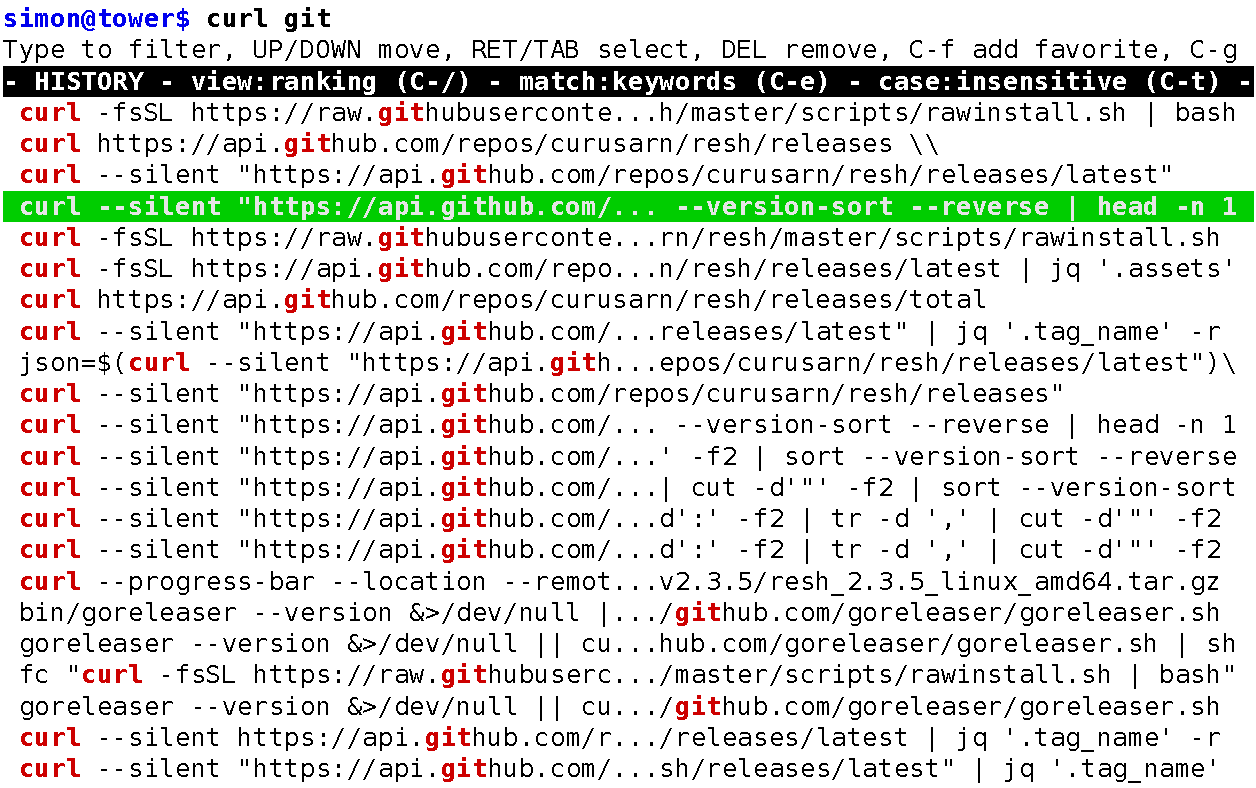
\includegraphics[width=0.995\linewidth]{figures/existing-tools/xterm-hstr-std.pdf}}
  \caption{Hstr interactive history search}
  \label{hstr-screenshot}
\end{figure}

\begin{figure}[h!]
  \permanentframe{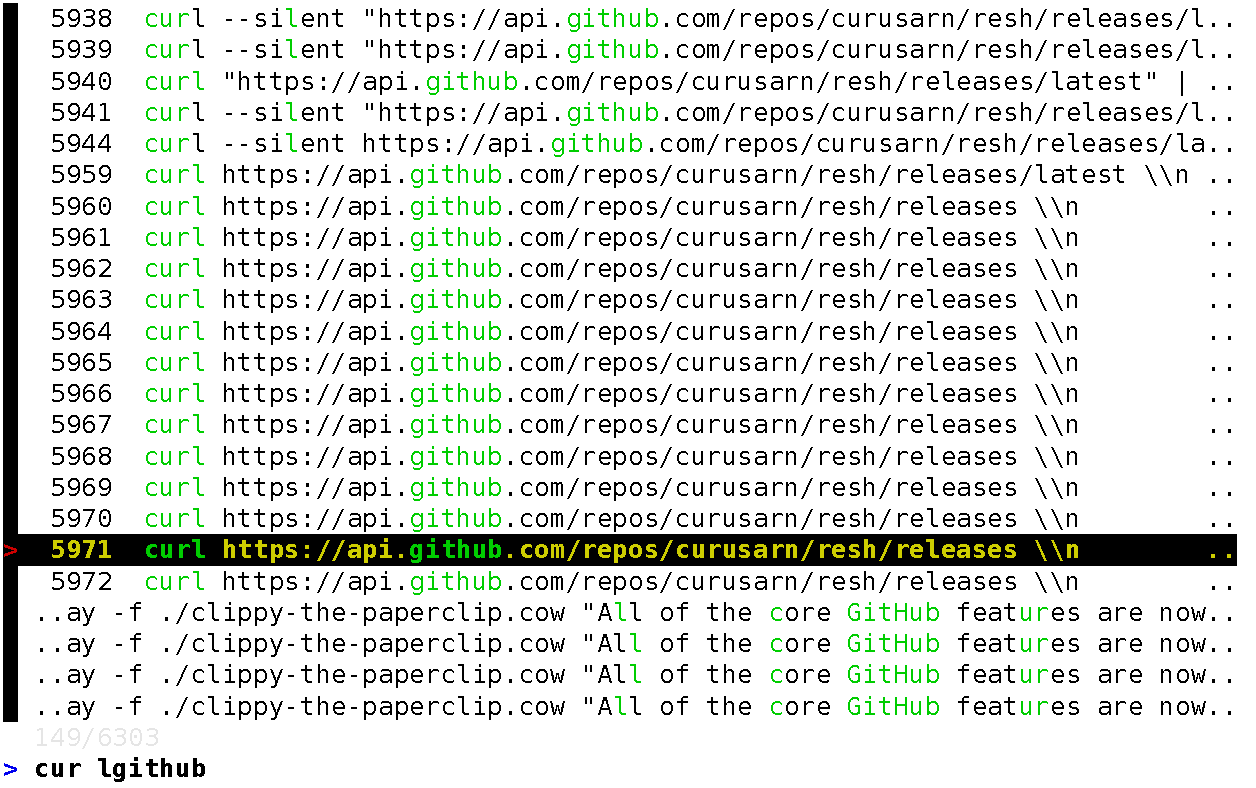
\includegraphics[width=0.995\linewidth]{figures/existing-tools/xterm-fzf-std.pdf}}
  \caption{Searching history interactively using Fzf}
  \label{fzf-screenshot}
\end{figure}

Fuzzy search is a commonly requested feature in various history tools. Some people who are already using Fzf cannot imagine using history tools without a fuzzy search.

\subsection{Contextual shell history in the cloud}


Bashhub\cite{toolsbashhubclient} saves your shell history to the cloud and allows you to search it from all of your machines.

Apart from the command line entry, Bashhub records and saves additional context. Each history record contains following:
\begin{itemize}
    %\setlength\itemsep{0em}
    \item command line entry
    \item exit status
    \item present working directory
    \item host
    \item time of execution
    \item ID of the session
    \item ID of the record
\end{itemize}

The Bashhub history search uses pattern matching\footnote{The pattern matching is implemented using SQL "LIKE" operator.} to search the submitted command line entries. The search can be restricted to the current directory and to the current host.


All searching is server-side; This means that every time you search your history using Bashhub, it needs to send a request to a remote server.
These requests take time, so there is no interactive "search as you type" functionality. Instead, you always have to type out the full query, execute the search command, and then wait for the results. Below, you can see an example of a search command that is restricted to the current directory. 

\begin{verbatim}
bh -d "curl git"
\end{verbatim}

An obvious disadvantage of a server-side search is that it does not work offline. 
When you use Bashhub, your history is saved on the remote server, and the server needs to be able to search it. This means that the history is on the server, at least in memory, in an unencrypted form. Adding client-side encryption would break the server-side search.

By default, the remote server is an instance maintained by the project author. The official server implementation is closed source. This means that you need to trust the author of the project with access to your shell history. 

Recently\footnote{Open source implementation of Bashhub server was written in February 2020.} a new open-source implementation\cite{toolsbashhubserver} of the Bashhub server has appeared. This addresses the privacy and security issues by making it possible to run and use your own instance of the server.

%\redtext{Bashhub is somewhat popular on GitHub\footnote{Bashhub has 744 "stars" on GitHub.}
%Bashhub is not a viable replacement for standard reverse search and manual history searching.}

\subsection{Contextual history search powered by a neural network}

McFly\cite{toolsmcfly} is a tool that tries to predict your next command line entry using a small neural network. It predicts the next command line entry based on the following contextual information:
\begin{itemize}
    \item present working directory
    \item previous command line entries
    \item how often you run the command line entry
    \item the last time you ran the command line entry
    \item if you selected the command line entry in McFly before
    \item exit status
\end{itemize}

Unlike Bashhub, this tool is designed to be bound to \verb|CTRL-R| and to replace the standard reverse search. Pressing \verb|CTRL-R| launches McFly full-screen terminal app shown in figure \ref{tools-mcfly}. At first, the app displays a list of ten predicted history entries. The list of history entries is updated as you type; It only shows results that exactly match the typed query. The list always contains ten results or less, which is a curious design decision. 


\begin{figure}[h]
  \permanentframe{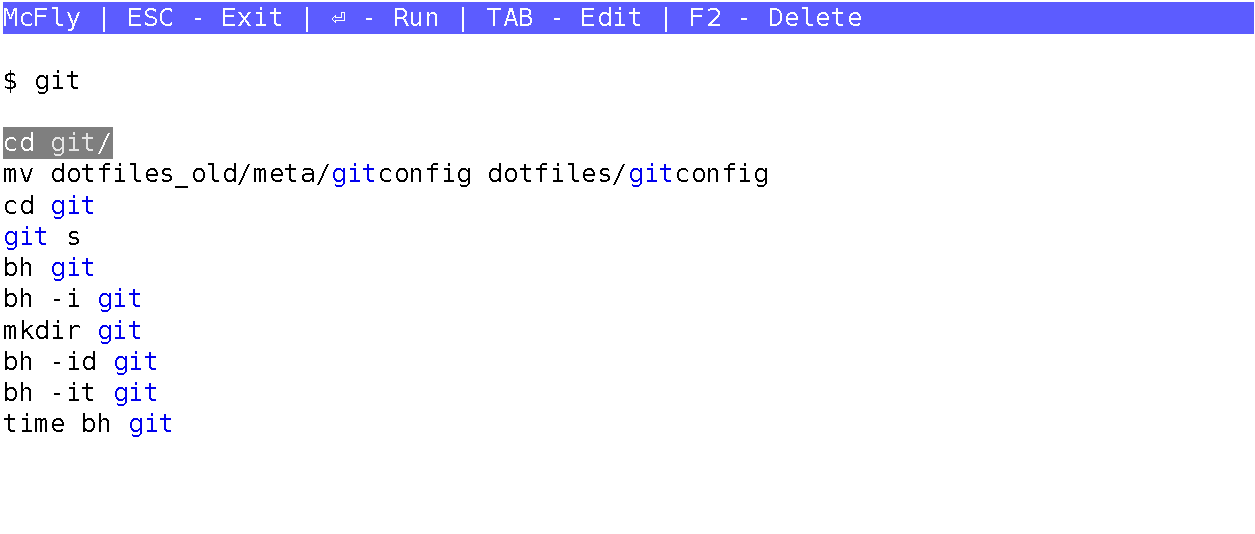
\includegraphics[width=0.995\linewidth]{figures/existing-tools/xterm-mcfly-std-short.pdf}}
  \caption{McFly interactive history search (cropped)}
  \label{tools-mcfly}
\end{figure}


When trying to use McFly, we found its behavior to be unpredictable; Not knowing why specific results are being shown made the tool less useful. 

McFly shares some problems with reverse search; It only uses a single query for searching. This can make it hard to find what you need in situations when you are unable to think of a better query\footnote{We already described such a situation in section \ref{workflow-search-w-limited-knowledge}}. 

%\redtext{McFly is popular on GitHub.\footnote{McFly has about sixteen hundred "stars" on GitHub.}}

%\begin{figure} \permanentframe{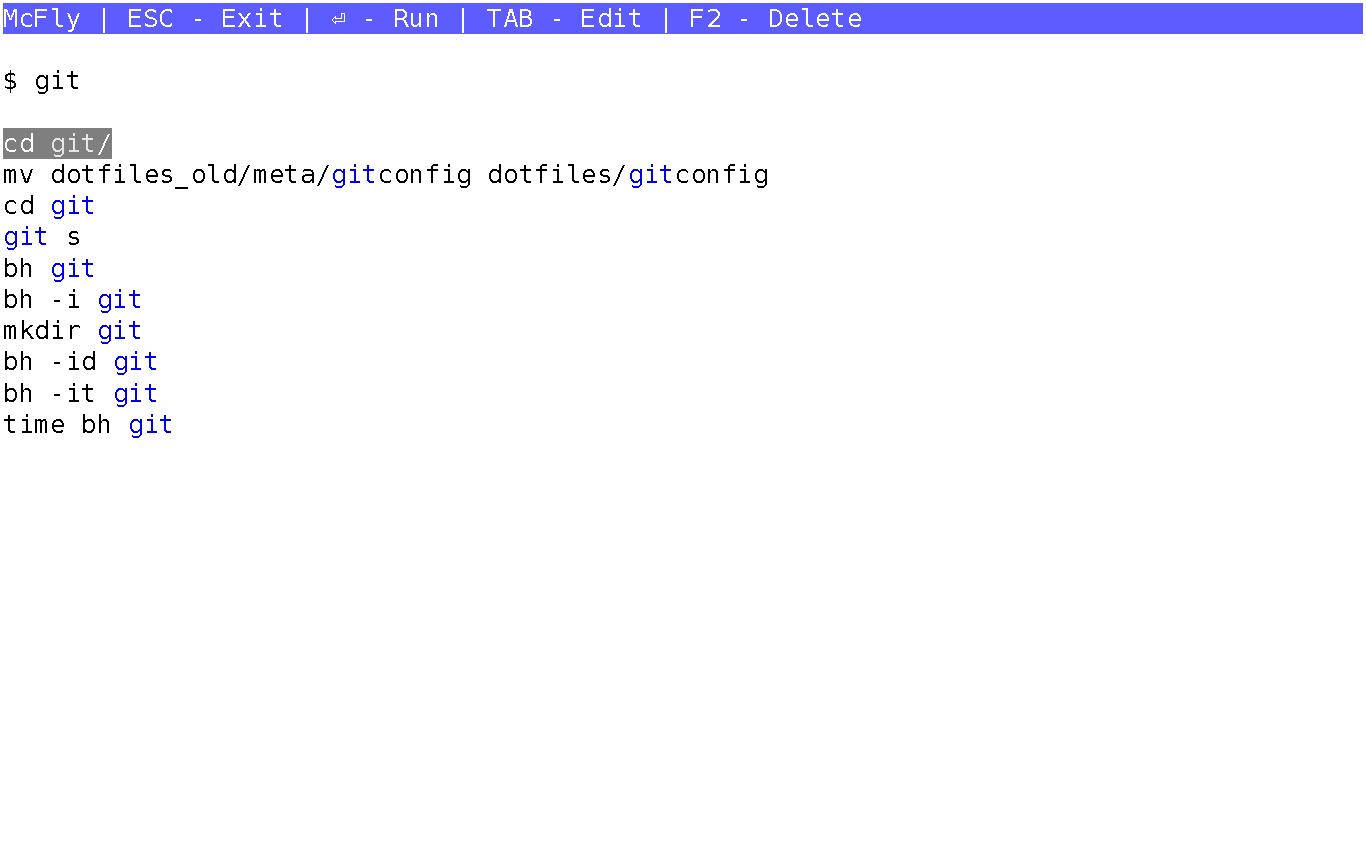
\includegraphics[width=0.995\linewidth]{figures/existing-tools/xterm-mcfly-full.pdf}} \caption{McFly interactive history search \redtext{REMOVE IMAGE}} \end{figure}


\section{Usefulness of contextual information}

In the previous section, we talked about existing history tools. We saw that contextual history tools are not automatically more useful than tools that do not work with additional context. 

Useful history tools address real workflows and provide value to the user.
In this section, we explore available contextual information. We will discuss how different parts of the context relate to shell usage and history usage. %We do this to identify the usefulness of different parts of available contextual information. 
We cover the following parts of the available contextual information:

\begin{itemize}
    \item Exit status
    \item Directory and Git related context
    \item Sequential relationships, sessions, and time
    \item Host and portability of history entries
    \item Usage of history features
\end{itemize}

\subsection{Exit status}

The shell interprets zero exit status as success. In contrast, non-zero status indicates failure.\cite{bashman} People often immediately edit and resubmit command line entries that returned an error. However, people probably rarely want to repeat older command line entries that failed. Does this mean that we can use exit status to filter out errors and only serve successful history entries to the user?

Not really, exit status does not directly map to success and failure. Programs can fail without returning an error. Some programs return non-zero exit status without actually failing\footnote{For example, GNU Grep returns one when no lines were matched and two to indicate errors.\cite{man-grep}}. 
Additionally, even history entries that are technically errors can be useful to the user. For example, the user might interrupt a program using \verb|CTRL-C| after it has fulfilled its purpose.

Generally, it is reasonable to assume that people retrieve history entries with zero exit status more often than the ones with errors. However, given the caveats described above, we should exercise this assumption conservatively. Removing history entries based on exit status would prevent the user from retrieving them. To preserve this ability, we can display all history entries but prioritize the successful ones.

\subsection{Directory and Git related context}

Directories provide explicit context. People change into different directories to complete different tasks.\cite{greenberg1993computer} It is often more comfortable to change directories compared to using longer paths as arguments. 

Many standard tools encourage the user to use specific directories for specific tasks. 
For example, Makefile, Vagrantfile, and Dockerfile are all designed to be used from within their directory\cite{man-make}\cite{docs-vagrantfile}\cite{docs-dockerfile}. 

Directories often hold projects that are associated with specific workflows and command line entries. 
These projects often use Git or other version control systems. This almost forces the user to use command line entries specific to the project inside the version control repository. 

We should make it easy to access the history entries from the present working directory.
However, we do not have to stop there. Directories and Git repositories are closely related, but they are not quite equivalent. Git provides some more context we can use. 
%The goal is to differentiate between history entries executed inside and outside the Git repository. 
Root of the Git repository allows us to group all history entries from the Git repository.
Git remotes\footnote{Remotes are remote repositories tracked by Git. Origin is the default remote.} can be used to identify the repository even across different machines or when it is moved to a different directory. 




\subsection{Sequential relationships, sessions, and time}

Command line entries are generally not executed individually; They are a part of longer sequences and tasks.\cite{greenberg1993computer} Each entry is related to its preceding and following command line entries. 

While analyzing shell history we collected from people, we observed significant sequential dependencies between command stubs. These dependencies represent workflows that users recognize and remember.\footnote{This specific analysis can be found in an appendix in section \ref{seq-app}.}

Apart from immediate sequential dependencies, each command belongs to a terminal session. We have observed significant differences between how people use sessions. Some people often create new terminals even for a few command line entries and then close them. Others keep terminals open for a long time and reuse them for different tasks.
Additionally, people very often switch back and forth between multiple open terminals. Command line entries from simultaneous terminal sessions are usually different but all related to the same task.

These relationships between history entries and sessions are definitely interesting and possibly useful. To illustrate, imagine you type a command line entry that you already executed five times in the past. Maybe it is related to a specific task, and to complete it, you will need similar commands as before. Situations like this one show us the potential usefulness of session and history entry relationships.

However, it is not apparent if these relationships are general enough to be useful in the average case. It is unclear how to use this complex contextual information to provide value to the user. It is beyond the scope of this work to study the relationships between history entries and between sessions.

Nevertheless, not all of the sequential contextual information is difficult to interpret and use. Sequences of history entries are useful because there are situations when people want to repeat them\footnote{We saw such a situation in section \ref{workflow-repeating-a-sequence} earlier}. We should support such workflows.

One more use for sequences of command line entries is recording them as a full non-deduplicated transcript. Having a full transcript of your actions gives you the ability to refer back to what you were doing earlier. A transcript of command line entries should also include the time of execution for the individual entries.

\subsection{Host and portability of history entries}

Imagine that you have your shell history synchronized between multiple devices.
Each of the devices is at least slightly different, so it is a good idea to be able to tell them apart. Devices usually have hostnames which we can use to identify them. 

Since each device can be different, we should look at the possible differences that are relevant to the shell history. Different operating systems use different package managers to install software. For example, Debian-based distributions use Apt, Arch-based distributions use Pacman, and on MacOS users use Homebrew. Commands for one package manager will not work with the others.

Many history entries are valid in both Bash and Zsh, but not all history entries. Shell configuration might differ between devices, which could cause some history entries to not work properly on all devices. A good example are specific shell aliases that the user added to one of their devices.

We just described why some history entries would not work when executed from a different device. Some history entries might not work even when executed on the same device but out of the original context. Examples of this are shell variables and relative paths. Variables that were set at the time of execution can cause history entries to fail when retrieved and executed again. History entries with relative paths will only work in specific directories.

As we can see, there are many reasons why history entries might not be portable. Most of the issues above can be detected using relevant contextual information. 
We could detect and handle these portability issues individually. Or alternatively, we could take a more straightforward approach; Prioritize history entries from the current device over those from other devices. This could be an effective strategy because many of the portability issues are related to mixing shell history from different devices. 

\subsection{Usage of history features}

So far, we have only described context related to the usage of shell and to the device. Now we look at the context that is related to how people use shell history. 

The first step is to know which command line entries are typed and which are retrieved from history. 
According to \cite{greenberg1993computer}, people tend to repeatedly retrieve the same events from history.

Next, we want to know which history feature was used to retrieve the entry. Knowing if the user used \verb|ARROW_UP| or \verb|CTRL-R| to retrieve a history entry allows us to separately study and evaluate these history mechanism. Different history features are used to complete different workflows; We should not treat them all as one.

%For example, when you retrieve a specific history entry using \verb|CTRL-R|, you are more likely to retrieve it using \verb|CTRL-R| again in the future.\footnote{We have observed that in collected usage data that retrieval of already retrieved history entries accounts for more searches than searching for the first time.}  

%This is supported by previous research; According to Greenberg, it should be it easy to retrieve history entries that were already retrieved earlier.\cite{greenberg1993computer}

A detailed transcript of user interactions with the history mechanisms would give us even more useful information. Consider a situation where the user presses \verb|ARROW_UP| ten times and then gives up and uses \verb|CTRL-R| to search the history instead. This is not an effective way to use history. However, it would be wrong to blame the user. If such a situation happens a lot to many users, we should look into if we can redesign \verb|ARROW_UP| to improve it.

The interactions between the user and the history features can help us understand how people use history. Knowing how people use standard shell history and our history solution is essential for informing design decisions. It is also crucial for evaluating the performance and usefulness of the final solution. %Interactions can help us understand when the system works and when it does not.



\chapter{Design}

In this chapter, we design our history system based on the previous analysis.
The design we present in this chapter is a result of an iterative process based on experiments and feedback from users. Designing user interfaces without iterative design often leads to usability issues.\cite{nielsen1993iterative}
    
We are designing new features to be integrated into shell and, by extension, workflows of people. Because of that, we need to respect the standard history features and the habits that people have built by using them. This is especially important for CLI features because they have low discoverability.\footnote{For example, if we add a new history feature to an unused key binding, there is no way for our users to discover it. Compare this with GUI application where available features can be displayed on the screen.}


The design should be simple and minimalist so that the user is not overwhelmed with available features. Overloading history mechanisms with complex functionality does not make them better.\cite{greenberg1993computer}


The first step of our design is to formulate requirements. These are based on previous analysis, workflows we identified, issues people have with standard history, and existing history tools. 

Second, we design the architecture of the history system. We describe what parts the system consists of. We also explain the purpose of these parts and the interactions between them.

%
Then, we focus on the interactive parts of our design. We explain the behavior we want the user to experience. The biggest interactive part of the system is an application that replaces standard reverse search. We design the visual layout of the application, keybindings, colors, and responsiveness. 

After that, we move on to the backend of the system. The backend includes the processes that support the interactive parts of the design. We show what data we need to handle and how we represent it.

Finally, we check and confirm that our design matches the initial requirements. For each requirement, we explain how our design fulfills it.


\newpage
\section{Requirements and features}


We selected following requirements based on the previous analysis:

\begin{itemize}
\item Record shell history with context and usage of history features
\item Allow history sharing between open sessions
\item Provide good out-of-the-box experience
\subitem Allow people to use the history system without configuring it first
\subitem Allow use of the system without reading manuals or help pages
\item Respect existing history features and existing habits of people
\subitem Do not change keybindings used for existing workflows
\subitem Support original workflows when replacing history mechanisms
\item Provide a replacement for reverse search
\subitem Solve the issues with standard reverse search
\subitem Match the few main improvements offered by Hstr and Fzf
\subitem Use recorded context to enhance history searching capabilities
\item Provide support for sequence repeating (forward in history)
\item Provide support for synchronization of shell history between devices
\item Provide support for contextual autosuggestions
\end{itemize}



\subsection{Basic features}

Now, we describe the basic features of the design. These features might seem obvious, but we point them out because they do contribute to the resulting usefulness of the history system.

History should be collected and recorded in a robust way; History should be unlimited, and using multiple simultaneous sessions must not result in missing history entries. 
Simultaneous sessions should be handled is a way that allows accessing history from other sessions.
All this has to work by default; No configuration should be necessary to achieve the basic functionality. 

The default configuration should provide good out-of-the-box experience for the average target user. It should not be necessary to read help pages or manuals to make use of the history system's main features. 
All new features should take the original habits of people into account. 
Introducing new or changing meaning of existing key bindings should be done with care. It is not easy for people to discover new key bindings in the shell.


\subsection{Core features}

The core focus of this design is providing a replacement for the standard reverse search. In this section, we explain why we chose this as the main focus of the design. We discuss how it relates to standard shell history features, existing state-of-the-art history tools, and possibilities of enhancing history searching with context.

%\paragraph{Standard history features}

Standard history features form the base that people are used to. We should not redesign and replace them unless we have a good reason to.
As we saw in the analysis, the standard reverse search does not provide a good feature set to complete many workflows. Furthermore, there are other tools available that provide features that solve the issues of reverse search. Because of this, we design a searching application that replaces and improves the reverse search.

%\paragraph{Matching the state-of-the-art}

Hstr\cite{toolshstr} and Fzf\cite{tools-fzf} are existing projects that replace reverse search and provide improved searching capabilities. 
Standard reverse search only uses a single query for searching and displays a single result at a time. In contrast, both of the tools mentioned above allow using more than a single query for searching and show a screen full of history results. We use these tools as an inspiration. Our searching application should match the key improvements provided by Hstr and Fzf. 

%\paragraph{Enhancing history searching with context}

In addition to matching the state-of-the-art features, we want to use context to enhance the searching capabilities of our history system. Our searching application should make it easier to retrieve history that match the current context. 


\subsection{Additional features}

Here, we describe features that are not the main focus of our design. These features are less important than providing a replacement for the reverse search. However, they are still valuable; We want to make sure they fit with the rest of the design. 
The chosen additional features are Forward in history, synchronizing history between devices, and Fish-like autosuggestions.



%\paragraph{Forward in history}

Forward in history is a feature we can find in Python console in Blender. We adopt this feature into our design because it allows the user to easily repeat sequences of history entries. Support for repeating sequences from history is poor in standard shell history.

%\paragraph{Synchronizing history}

Synchronizing history between multiple devices is an appealing feature. It enables history reuse between devices. The potential for reuse is further enhanced by using context to prioritize the search results.
Synchronized history is also harder to lose because it is replicated across multiple devices. 

%\paragraph{Autosuggestions}

Autosuggestions are a very convenient and very fast history mechanism. Original Fish autosuggestions use context to determine what history entry should be displayed.
We want to include a similar feature in our design.

\newpage
\section{Architecture}

In the previous sections, we listed all the features that we chose to include in the design. We chose a set of features that fits well together and should significantly improve the usefulness of shell history.

Now, we design the architecture of our history system so that it can accommodate all the features. 
Our history system consists of a daemon and multiple components. The daemon is always running in the background. Components are integrated into the shell and activated at appropriate times. 

%\paragraph{Daemon}

Daemon allows us to asynchronously preprocess the history data and serve it to the components when it is needed. It is responsible for loading and saving history to the storage. Daemon gives us the option to easily share history between sessions. History synchronizations is initiated and controlled by the daemon.

%\paragraph{Components}

Multiple different components are activated at various times based on their purpose. The history collector records the shell history with context and sends it to the daemon. Autosuggestion and arrow keys handlers respond to the interactions with the user. Finally, the search application interacts with the user, communicates with the daemon, and does its own share of data processing.


For the purpose of this design, we divide the system into two logical sections: frontend and backend. As you can see in figure \ref{design-architecture-layers}, the frontend is responsible for the interactions with the shell, terminal, and by extension, the user. Backend is mostly about handling data. 

\begin{figure}[h!]
\centering
\tmpframe{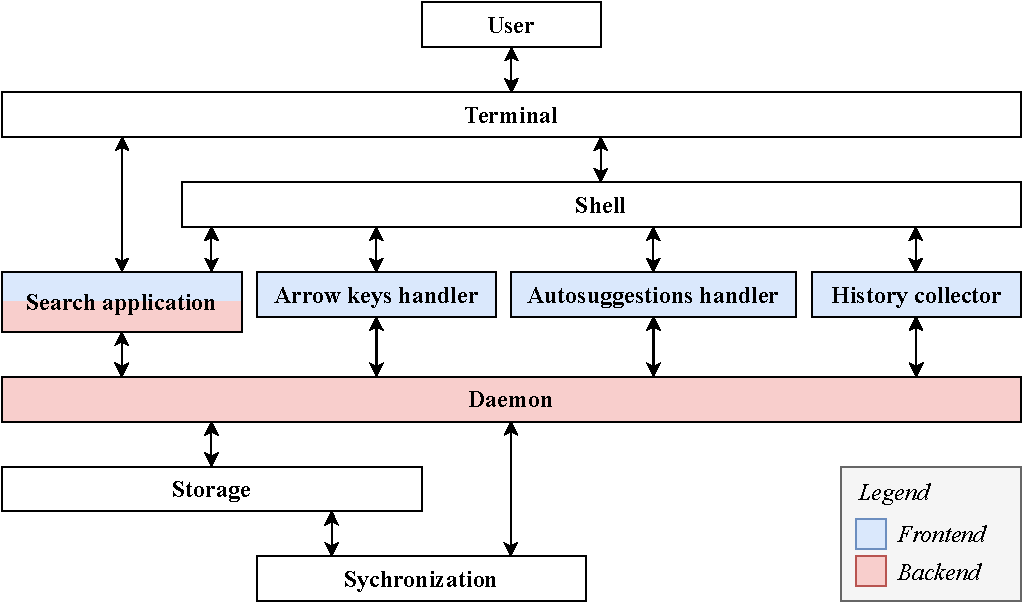
\includegraphics[width=\linewidth]{figures/design/thesis-design-architecture-layers-v2.pdf}}
\caption{Schema of architecture and communication}
\label{design-architecture-layers}
\end{figure}

\newpage
\section{Frontend}\label{design-frontend}

In this section, we focus on and design the parts of the system that the user interacts with. 
To relate this to our previous analysis, these are the specific workflows we are addressing in this section:

\begin{itemize}
\item Searching with limited knowledge (section \ref{workflow-search-w-limited-knowledge})
\item Searching with implicit context (section \ref{workflow-search-w-implicit-context})
\item Repeating a sequence of history entries (section \ref{workflow-repeating-a-sequence})
\end{itemize}

\subsection{Search application}

The most important part of our design is the replacement for standard reverse search -- a full-screen terminal history searching application. The application is inspired by Hstr and Fzf. 

We start by designing the visual layout of the application.
The wireframe in figure \ref{wireframe-normal} shows the layout of the default view of the application. There are three sections in the wireframe:

\begin{itemize}
\item Search input
\item Main section with search results
\item Status bar with details and help
\end{itemize}




The search results in the main section are interactively updated as the user types into the search input. Table \ref{tab:design-columns} shows which context is always visible and which is only displayed when relevant. Git repository and exit status both share the same column ("FLAGS"). 

\begin{table}[h]
\centering
\begin{tabular}{lllll}
\hline \hline
Context & Header & When visible \\\hline
Time/date & TIME & always \\ 
Host & HOST & only for history from other hosts \\ 
Directory & DIRECTORY & always \\ 
Git repository & FLAGS & only for history from this git repo. \\ 
Exit status & FLAGS & only non-zero exit status \\ 
Command line & COMMAND-LINE & always \\\hline \hline
\end{tabular}
\caption{Context and columns in the default view}
\label{tab:design-columns}
\end{table}

Host and directory also share a single column, but they do have separate headers. Columns are being dynamically resized to fit the data and to not waste space. Command line entry, host, and directory are shortened to fit the screen if necessary. 

Near the bottom of the screen, there is a status bar with details about the currently selected entry and help. These details are displayed without any shortening, and the status bar is expanded to accomodate them. Under the command details, there is help that shows key bindings and other information.


The wireframe in figure \ref{wireframe-detail} shows the detail view. In this view, the user can see the details and surrounding history entries for a single command line entry. Each command line entry can appear in history multiple times; The user can switch between these occurrences. The next occurrence is partially displayed to make it easier to compare the surrounding history entries.


\paragraph{Key bindings}
When designing key bindings, it is essential to respect existing key bindings and to leverage what are the users already used to.
We want to avoid collisions with flow control keybindings so we do not use \verb|CTRL-S| and \verb|CTRL-Q|. Additionally, we do not reuse standard job control key bindings \verb|CTRL-Z|. 
Since we are replacing the reverse search, we are following many of its key bindings. The list of keybindings for our history search application follows:

\begin{itemize}
\item \verb|CTRL-R| to launch the search application from the command line
\item Type to search
\item \verb|ARROW_UP|/\verb|ARROW_DOWN| to select 
\item \verb|ARROW_RIGHT| to paste the selected entry to the command line for editing
\item \verb|ENTER| to execute the selected entry
\item \verb|CTRL-X| to show detail view for the selected entry
\item \verb|CTRL-C|/\verb|CTRL-D| to quit
\item \verb|CTRL-G| to abort and paste the current search query onto the command line
\end{itemize}


\paragraph{Scaling in larger terminals}

Both wireframes above both use the standard 80x25 character terminal size. In larger terminals, there is more space that can be used. Columns with hosts, directories, and command line entries stretch to make use of the extra space. The main section with search results becomes longer, and consequently, more history entries fit in the terminal. 

\paragraph{Colors}

Our application has a lot of information to display. 
Colors are used to highlight the information that influences the order of displayed results. To make it easier to differentiate between different types of information, they are highlighted using different colors. 
The red color is reserved for highlighting remote hosts and non-zero error status; This communicates to the user that these history entries might not work well.
Currently selected history entry is highlighted by inverting the foreground and background colors.



\begin{figure}[h!]
\permanentframe{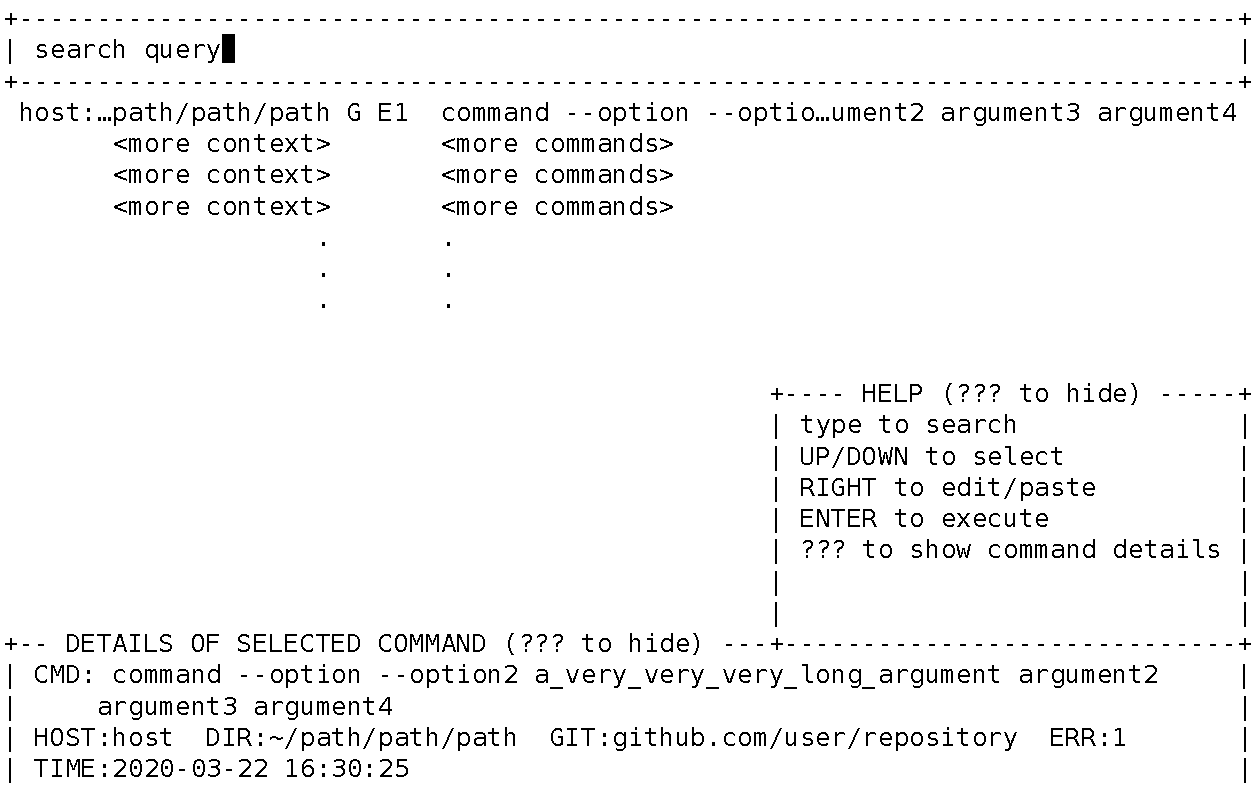
\includegraphics[width=0.995\linewidth]{figures/design/xterm-wireframe-bw-normal.pdf}}
\caption{Wireframe of default view}
\label{wireframe-normal}
\end{figure}

\begin{figure}[h!]
\permanentframe{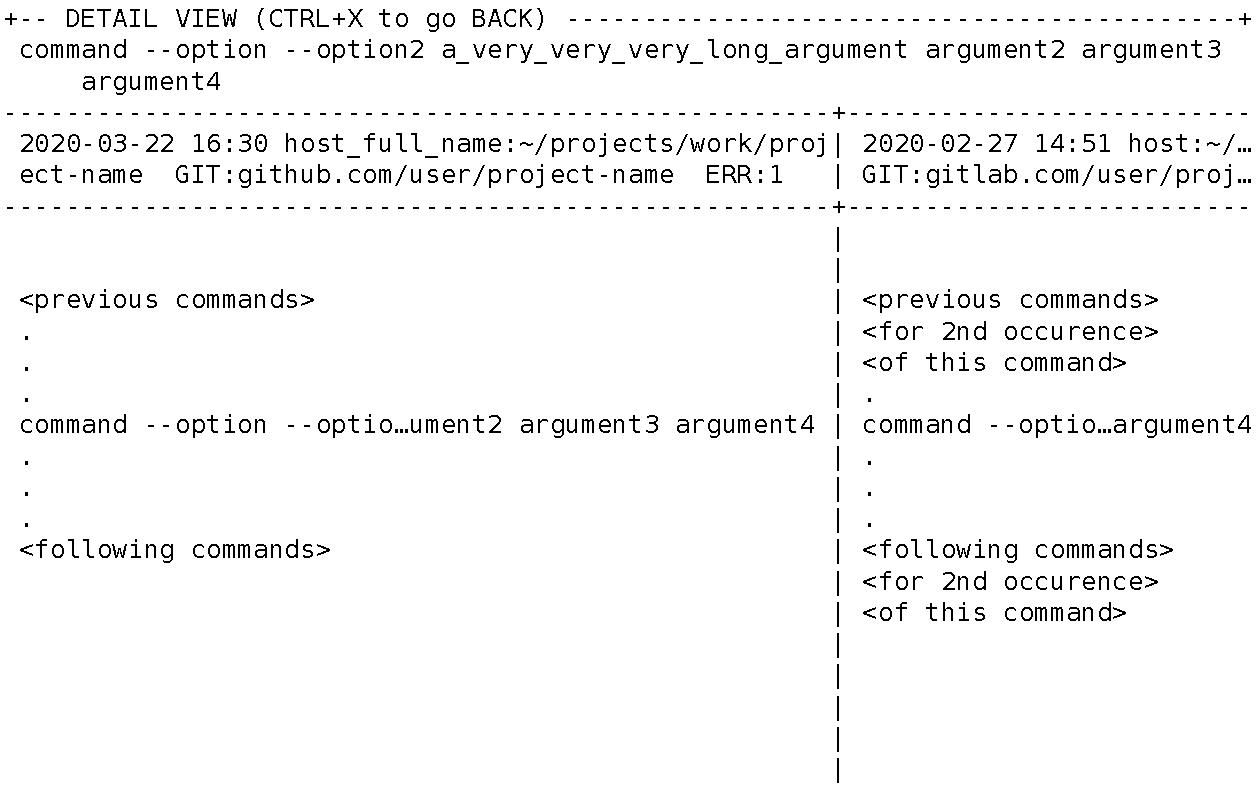
\includegraphics[width=0.995\linewidth]{figures/design/xterm-wireframe-bw-detail.pdf}}
\caption{Wireframe of detail view}
\label{wireframe-detail}
\end{figure}


\subsection{Arrow key handler}

Our previous analysis found out that standard history mechanisms available via arrow keys work reasonably well. Furthermore, people have a strong expectation of seeing recent history entries on \verb|ARROW_UP|. 
For these reasons, we only introduce minor changes into the standard behavior of arrow keys.


In our design, the prefix history search is enabled by default. It is a useful feature that does not interfere with the standard stepping through history. Additionally, the history available via \verb|ARROW_UP| is fully deduplicated.

\paragraph{Forward history}

In standard shell history, \verb|ARROW_DOWN| is without function unless we press \verb|ARROW_UP| first. It is only useful as a way to get back from recent history to the original command line.

We overload \verb|ARROW_DOWN| with an additional feature - Forward in history. When previously executed command line entry was retrieved from history, pressing \verb|ARROW_DOWN| gives the user access to the next history entry in the sequence. 
The user can easily repeat whole sequences because each history entry in the sequence can be retrieved by a single press of \verb|ARROW_DOWN| and then executed. 


To preserve the ability to hold \verb|ARROW_DOWN| to return from recent history to the original command line, we introduce a delay. A delay in activation of forward history feature that is triggered when the user holds down \verb|ARROW_DOWN| while in recent history.

\subsection{Autosuggestions handler}

Autosuggestions in our history system use the recorded context to recommend history entries to the user. The suggested history entry is determined based on the current context. History is searched for matching entries in this order:

\begin{itemize}
\item history from the current directory
\item history from the current git repository
\item history from the current host
\item history from anywhere
\end{itemize}

Additionally, we introduce an exception to enhance the Forward in history feature. 
When the user uses \verb|ARROW_DOWN| the next autosuggestion should try matching a few next history entries in the history sequence before any other history entries. 

\section{Backend}

In previous sections, we focused on the parts of the system user interacts with.
Now we design the inner workings of the system that make it possible to provide the desired behavior to the user.

\subsection{Search algorithm}

The terminal history searching application needs to serve relevant entries to the user based on the query and current context. When searching, each history record is assigned a score. This score is based on how well history record matches the query, how well it matches the current context, and also on its time of execution. 

After scoring all the history records, they are sorted. Finally, history entries with the highest scores are displayed to the user.

\paragraph{Scoring metric}

The score for a record \(r\) with query \(q\) and current context \(c\) is a sum of three parts: 

\[ Score_r(q,c) = w_1 \cdot QueryScore_r(q) + w_2 \cdot ContextScore_r(c) + w_3 \cdot TimeScore_r \]

The score weights \(w_1\), \(w_2\), and \(w_3\) determine how the parts of the score relate to each other. 

The first part, \(QueryScore\), represents how well the history record matches the query typed by the user. It is essential that \(QueryScore\) has the most influence over the total resulting score. Not giving enough weight to it could lead to situations where the user types in a query, but the displayed results match the context instead. 

The second most important part is \(ContextScore\); It represents the similarity between the context of the history record and the current context. Finally, \(TimeScore\) gives higher scores to more recent history entries. The influence of \(TimeScore\) on the total resulting score should be marginal.

Now that we covered how the partial scores relate to each other, we look at them individually.

\paragraph{Query score}

To calculate the \(QueryScore\), the query provided by the user is broken down into individual words. 
Each word is matched against the command line entries separately. Each query word also independently contributes to the score. This means that as the user adds more words to the query, the influence of the context becomes less and less significant.

We formalize this property as follows; Let queries \(q_1\) and \(q_2\) be represented as sets of individual words. For any queries \(q_1\), \(q_2\) and any history record \(r\): 

\[ q_1 \subset q_2 \Rightarrow QueryScore_r(q_1) \leq QueryScore_r(q_2)\]\

\paragraph{Context score}
The second part of the total score is \(ContextScore\); It takes the current context at the time of execution of the search application and compares it to the context of individual history records. 
The current context is compared with the context of the history records using four conditions displayed in the table \ref{tab:score-matching-context}. As shown in the table, each of these conditions either increases or decreases the score.

\begin{table}[h]
\centering
\begin{tabular}{lll}
\hline \hline
Context condition & Effect \\
\hline
Directory matches & significantly increase score \\ 
Git repository matches & increase score \\ 
Non-zero exit status & decrease score \\
Host does not match & slightly decrease score \\ 
\hline \hline
\end{tabular}
\caption{Influence of different parts of context on \(ContextScore\)}
\label{tab:score-matching-context}
\end{table}

To make it easy to skim over displayed results in the search application, we want the results to be grouped based on context when possible. 
We want to prevent history records with different contexts from being unnecessarily mixed together. 
To achieve that, \(ContextScore\) should be an injective function of the history record context.

In other words, any two history records \(r\) and \(s\) with different contexts never share the same \(ContextScore\) for a given current context \(c\):
\[ context_{r} \neq context_{s} \Rightarrow ContextScore_r(c) \neq ContextScore_s(c) \]\
Here, \(context\) of history record \(r\) is defined as its directory, git repository, exit status, and host:
\[ context_r = (directory_r, gitRepository_r, exitStatus_r, host_r) \]

\paragraph{Time score}

The last part of the score is \(TimeScore\). It is the least important of the partial scores. The most recent entries have the highest \(TimeScore\), and older entries have lower \(TimeScore\). 

\paragraph{Score weights}

We described the scoring function as a whole. We also introduced some important properties of the partial scoring functions. However, the resulting behavior of the whole scoring function depends on the concrete weights we use. 
Specific weights should be determined experimentally based on real-life shell history.

\subsection{History synchronization between devices}

Instead of implementing our own dedicated synchronization server, we design our history system to rely on third-party services for synchronization. 

The process of synchronization works like this: First, we check if there are any new history entries. If so, we download them and merge them into local history. Finally, we check for new history again, and if there is none, we upload the newly merged history. 

The daemon controls this whole synchronization process; It initiates the individual steps and handles when they fail. It also takes care of the history merging. Download, upload, and checking for new history is not part of the daemon. These three steps are different for each synchronization service; They are extracted out of the daemon and combined into a "Synchronization connector". Each synchronization connector provides support for a single synchronization method. Synchronization connectors do not contain any complicated logic. 


\subsection{Data representation}

In this section, we discuss what data we need to handle and how it should be represented so that all the chosen requirements and features are possible.


Contextual shell history is inherently relational. Each history record was executed as part of a given session, on a host, in a specific directory. However, we do not need the relational properties of the history for most of the features. For example, when searching, we need to calculate scores for all history entries, not just the ones with matching context. 

We represent the data as a stream of history records. Each record can be uniquely identified by its ID. Separate entries are very easy to merge when we synchronize history from multiple devices.

Based on all requirements and features of our design, each record has to contain at least following data:
\begin{itemize}
\item machine ID
\item session ID
\item record ID
\item time of execution
\item host
\item directory
\item git repository
\item exit status
\item command line entry
\item usage data / user interactions
\end{itemize}



\begin{figure}[h!]
\centering
\tmpframe{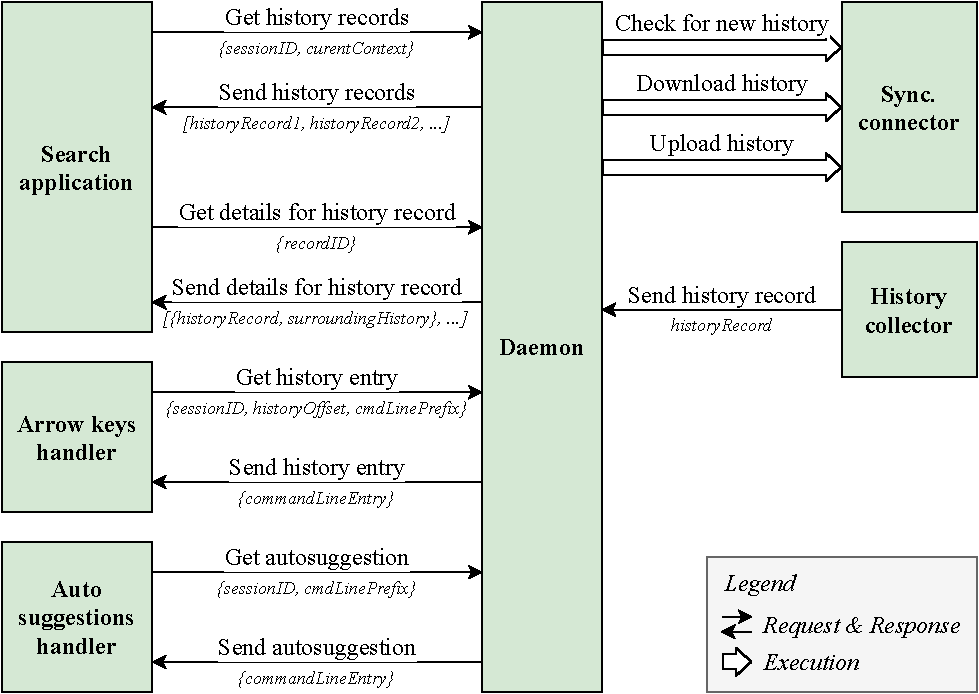
\includegraphics[width=\linewidth]{figures/design/thesis-design-api.pdf}}
\caption{Schema of communication and exchanged data}
\label{design-api}
\end{figure}


\subsection{Communication}

Here, we describe the communication between the components of our history system. Figure \ref{design-api} shows requests, responses, and execution that happen in the system. Data that is sent with each request is displayed under the arrow. 

The search application requests all history records when it is launched and then requests details for a specific history record when the user switches to the detail view. Response with the details for the history record contains a list of occurrences of the command line entry. Each occurrence consists of the history record and surrounding command line entries.

Arrow key handler is simpler; It requests a history entry based on the current session, the prefix that is already typed on the command line, and history offset that represents how many times did the user press the arrow key. The response is a single command line entry to display.

Autosuggestions handler requests a command line entry to show. The request contains a session ID and the prefix that the user already typed on the command line.

All of these components are integrated into the shell and activated when a specific key is pressed. Furthermore, they directly manipulate the contents of the command line when they return a command line entry to the user.

The history collector is also integrated into the shell so that it can collect the current context and send it to the daemon. Synchronization connector does not receive any data; Instead, it is executed by the daemon to complete low-level synchronization tasks. 

\section{Design testing}

In this section, we test out design to make sure that we covered all the requirements. We go through the requirements one-by-one and argue why our design fulfills them. 

\begin{itemize}
\item Record shell history with context and usage of history features
\end{itemize}

History collector records the history with context and usage and sends it to the daemon.

\begin{itemize}
\item Allow history sharing between open sessions
\end{itemize}

Daemon handles all of the history records so it can send it to any component regardless of sessions.

\begin{itemize}
\item Provide good out-of-the-box experience 
\subitem Allow people to use the history system without configuring it first
\subitem Allow use of the system without reading manuals or help pages
\end{itemize}

Our design does not expect people to configure the system before using it. Designed behavior is based on previous research and target users. Information required to use the search application is presented inside of it. There are features that are harder to discover, but these are not essential for the most common workflows. 

\begin{itemize}
\item Respect existing history features and existing habits of people
\subitem Do not change keybindings used for existing workflows
\subitem Support original workflows when replacing history mechanisms
\end{itemize}

We redesigned the behavior of standard history while keeping the original workflows intact. Recent history is still accessible on \verb|ARROW_UP| in unchanged order. People can still use \verb|CTRL-R| for general-purpose history searching. 
The search application supports the workflows of standard reverse search.

\begin{itemize}
\item Provide a replacement for reverse search
\subitem Solve the issues with standard reverse search
\subitem Match the few main improvements offered by Hstr and Fzf
\subitem Use recorded context to enhance history searching capabilities
\end{itemize}

Our history searching application provides features that are a superset of what the reverse search provides. It can search for anything that reverse search can because the query is designed to have the most influence over the scoring function.

Reverse search only uses a single query and shows a single result. This significantly reduces its usefulness. Our searching app uses multiple word queries and shows a page full of results. These are also the main improvement provided by the Hstr and Fzf.
The search application searches history based on both query and current context.

\begin{itemize}
\item Provide support for sequence repeating (forward in history)
\item Provide support for synchronization of shell history between devices
\item Provide support for contextual autosuggestions
\end{itemize}

Our design includes support for forward history. Forward in history is a feature that makes it possible to easily repeat sequences. 
The daemon and the synchronization connectors provide support for synchronization between devices. The autosuggestions handler provides support for contextual autosuggestions.




\chapter{Implementation}

In the previous chapter, we designed a history system based on our previous analysis. Now we describe the actual implementation. 

We did not implement every part of the design because it is quite extensive. Instead, we chose parts of the design that bring the most value to users. Naturally, we also implemented parts of the design that are required for the system to actually work.

First, we identified the search application as the most important part of the design to implement. Second, we wanted to collect the usage of shell history. To implement these two parts of the design, we needed to implement many other things. 

We need to integrate with the shell to collect history, context, and usage. Arrow key bindings are necessary to collect their usage. The search application also needed its custom key bindings. Daemon is necessary to process, save, load, and serve history data. Additionally, we also needed a convenient way to release the project and to deliver it to users.

\section{Shell integration}

In this section, we describe how our history system integrates into the shell so that is can provide the required functionality. 

\subsection{History collector}

Standard history does not contain context, so we need to record it ourselves. 
We need to record contextual information both before and after the command line entry is executed. Most of the context is recorded before the execution, but some context such as exit status is only available after the execution. 

We have two shell functions that record the context and send it to the daemon. One is called before and one after command line entry execution. In Zsh, we used \verb|preexec| and \verb|precmd| hook functions to make Zsh call our functions at appropriate times. 

In Bash there are no native \verb|preexec| and \verb|precmd| hook functions. Luckily, there is a library \cite{lib-bash-preexec} that emulates these hook functions in Bash. The behavior is not always quite the same as in Zsh, but we managed to work around all the issues we encountered with Bash. 

\subsection{Key bindings and line editing}

For many components of our history system, we need a way to bind custom shell functions to keys so that they are launched when a key is pressed. We also need to be able to manipulate the contents of the command line from these functions.

Zsh and Bash both have their own different built-in commands that allow us to bind shell functions to keys. Both shells also provide a different way to manipulate the command line contents. Ideally, we do not want to pollute our code base with many lines of shell specific code.

Unluckily, we could not find any library that provides a unified key bindings interface. Because of that, we created a library\cite{lib-bash-zsh-compat-widgets} that allows the same shell function to be bound to keys and used for command line editing in both Zsh and Bash. Additionally, the key bindings can be reverted to restore the original function.
We used this library to implement arrow key bindings that imitate the default behaviour.

% Bash issues and limitations 

% \subsection{Arrow key handler and collecting usage}

\section{Search application}

In this section, we describe the implementation of the notable parts of the search application. 

\subsection{Overview}

First, we look at the sequence of actions that happens when the search application is used. The sequence diagram in figure \ref{impl-search-app-sequence} shows the interactions of the user with different parts of the system.

At the start of the diagram, the user presses \verb|CTRL-R| while on the shell prompt. Shell calls our custom shell function that wraps the search application. The shell function collects the current context and executes the search application; The context is passed using command line arguments. 


\begin{figure}
\centering
\tmpframe{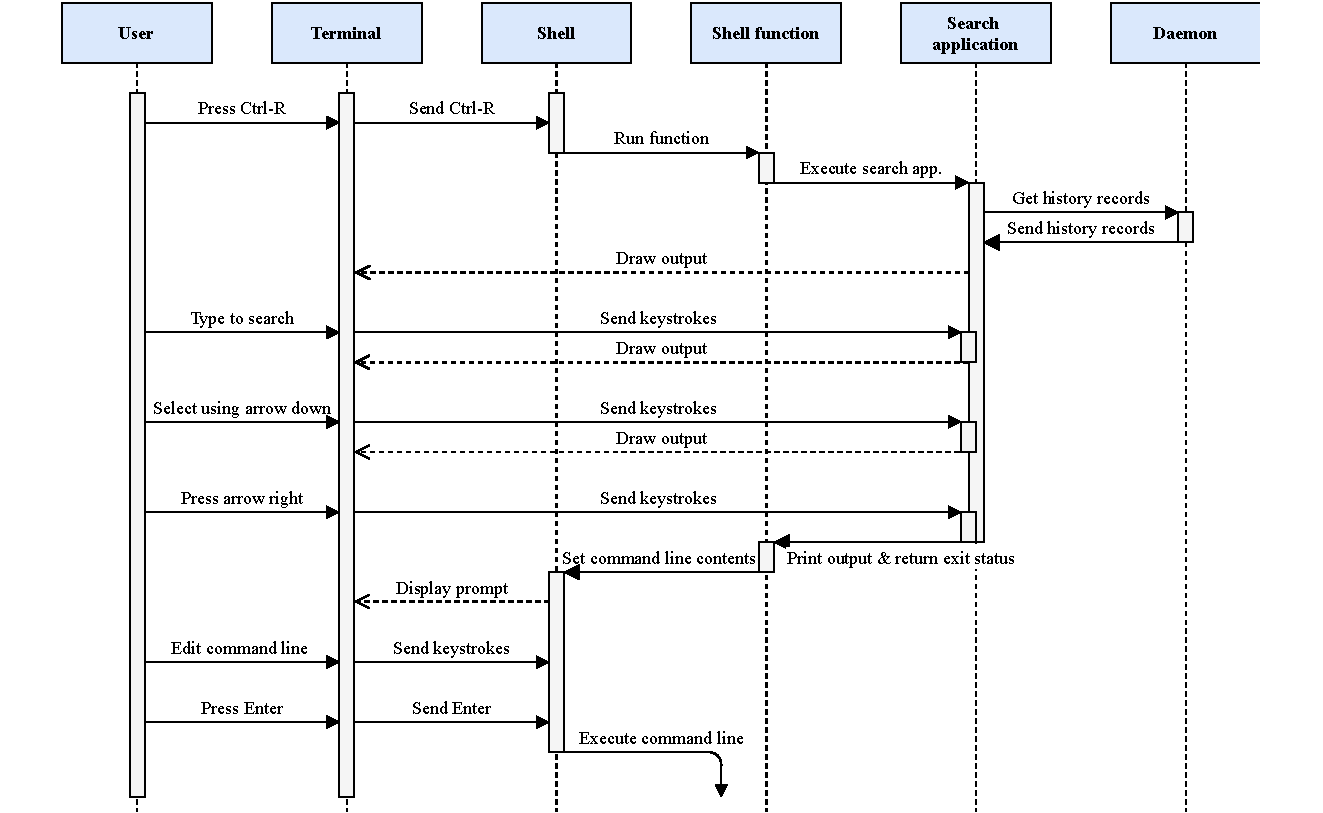
\includegraphics[angle=90,origin=c,width=\linewidth]{figures/implementation/thesis-impl-search-app-sequence-PADDING.pdf}}
\caption{Sequence diagram of using the search application}
\label{impl-search-app-sequence}
\end{figure}


The search application gets the history records from the daemon, searches the history, renders the results, and draws output to the terminal. We use a library\cite{lib-gocui} for creating terminal applications. This library takes care of drawing the output to the terminal and handling key bindings. Every time the user types something or presses any keys in the search application, the history is searched again, and the results are rendered. 

When the user accepts the selected history entry, the application prints it to standard output and returns an exit status. 
The shell function captures the selected history entry; The history entry is written onto the command line. Based on the exit status, the shell function either executes the history entry or leaves it for the user to edit. The sequence diagram in figure \ref{impl-search-app-sequence} shows the latter. 

After the selected history entry is pasted onto the command line, the user can further edit it. 
It is possible to use all standard editing capabilities of the shell to edit the command line.
Once the user accepts the command line, the shell evaluates and executes it.




\subsection{Rendering}

The previous section covered how the search application interacts with the user and how it is launched from the shell. Now we describe the rendering process that happens inside the search application.


In figure \ref{impl-search-app-render-pipeline}, we can see a schema of the rendering pipeline. This pipeline is triggered as a response to any change in the search query made by the user. 


First, scores are calculated for all the history records. Then, the records are sorted by the score and filtered based on how many rows fit in the terminal. After that, we render columns for history records that will be visible on the screen. At this point, we determine how wide the individual columns should be. Finally, we put the columns together to render the full lines that are displayed in the application.


\begin{figure}[h!]
\centering
\tmpframe{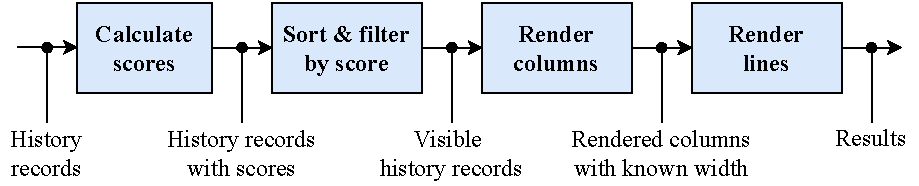
\includegraphics[width=\linewidth]{figures/implementation/thesis-ipml-rendering-pipeline.pdf}}
\caption{Schema of rendering pipeline in the search application}
\label{impl-search-app-render-pipeline}
\end{figure}



Now that we know how the rendering process works, we can look at the screenshots from the search application. In figure \ref{xterm-resh-normal-80}, we can see that the individual columns only take as much space as they need. 

The second screenshot in figure \ref{xterm-resh-normal-80-long} shows how the contents in the host and directory column are shortened. This happens when the contents are too long relative to the terminal width. The command line column takes up the rest of the terminal width. All shortened information for the selected result is displayed on the status line in full. 

In larger terminals, a less compact time format is used; This is shown in figure \ref{xterm-resh-normal-full}.


\newpage
\begin{figure}
\permanentframe{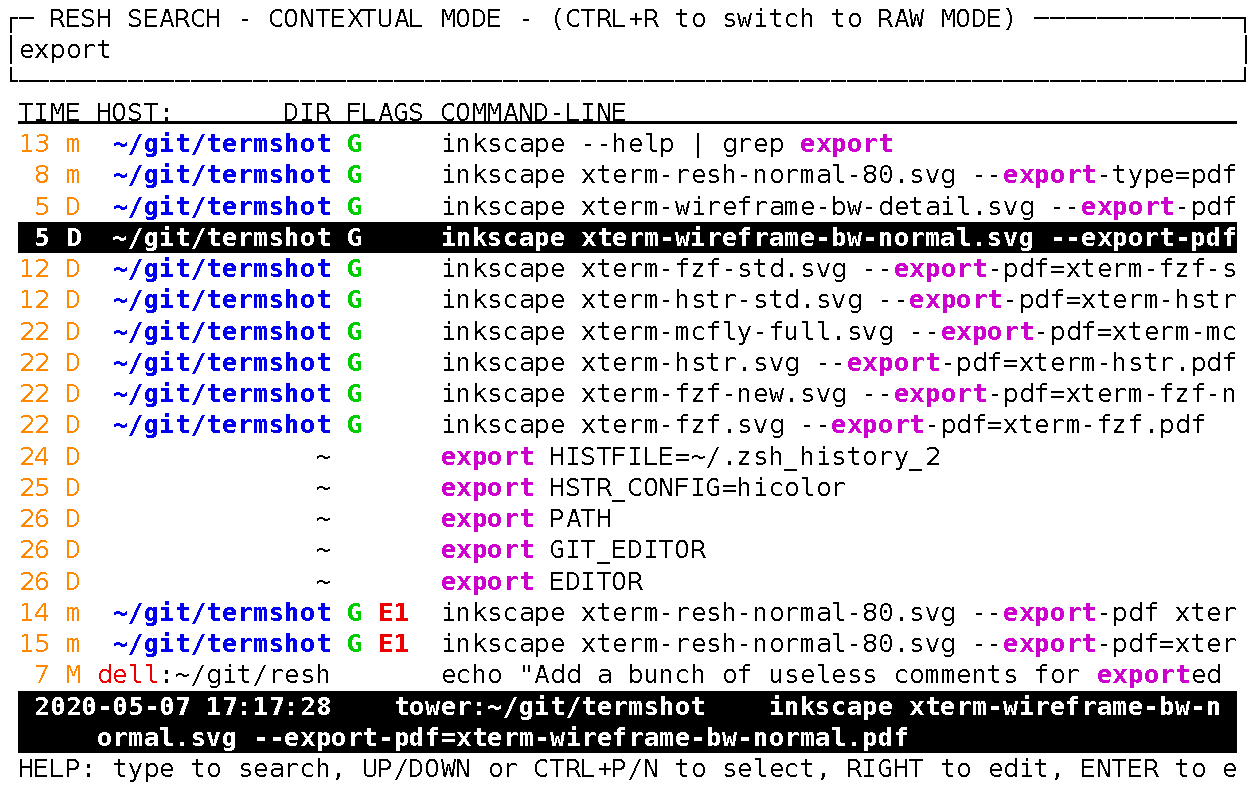
\includegraphics[width=0.995\linewidth]{figures/implementation/xterm-resh-normal-80.pdf}}
\caption{Screenshot of the search application in the standard terminal size}
\label{xterm-resh-normal-80}
\end{figure}

\begin{figure}
\permanentframe{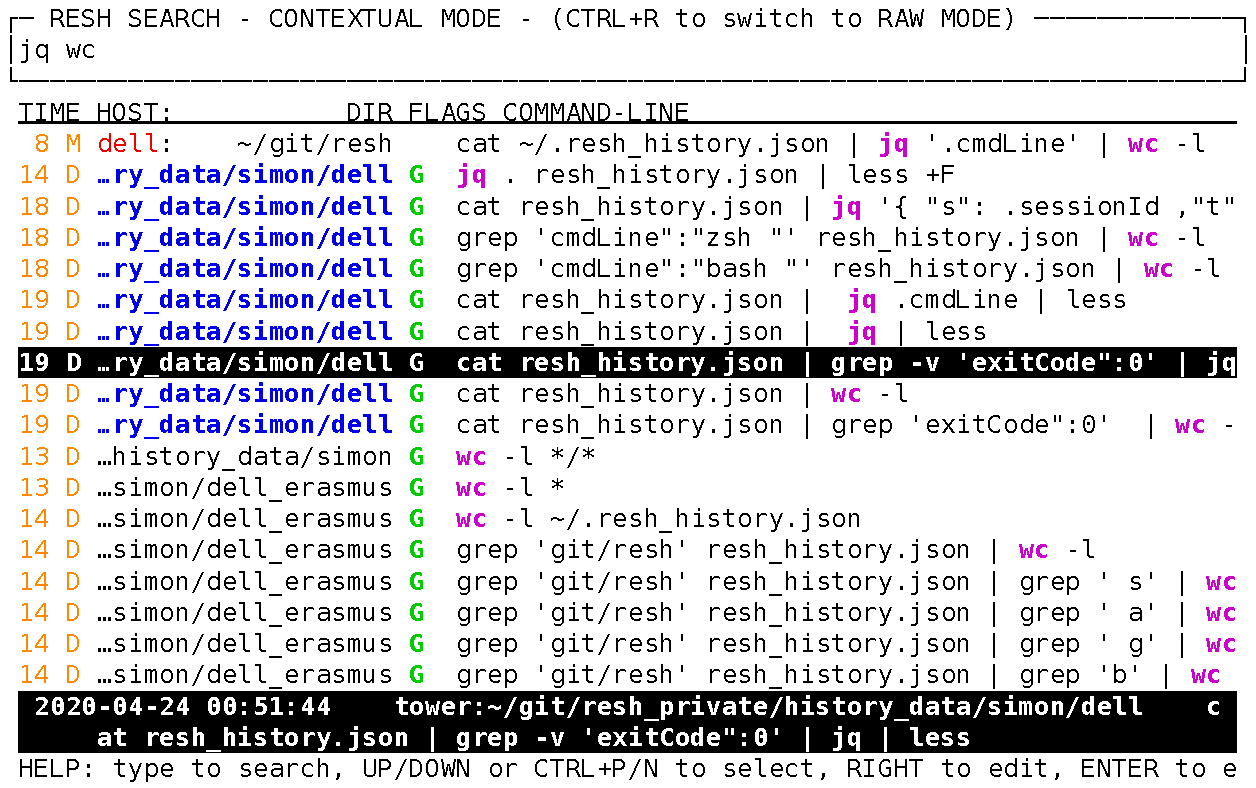
\includegraphics[width=0.995\linewidth]{figures/implementation/xterm-resh-normal-80-long.pdf}}
\caption{Screenshot of the search application with wide columns}
\label{xterm-resh-normal-80-long}
\end{figure}

\newpage
\begin{figure}
\centering
\permanentframe{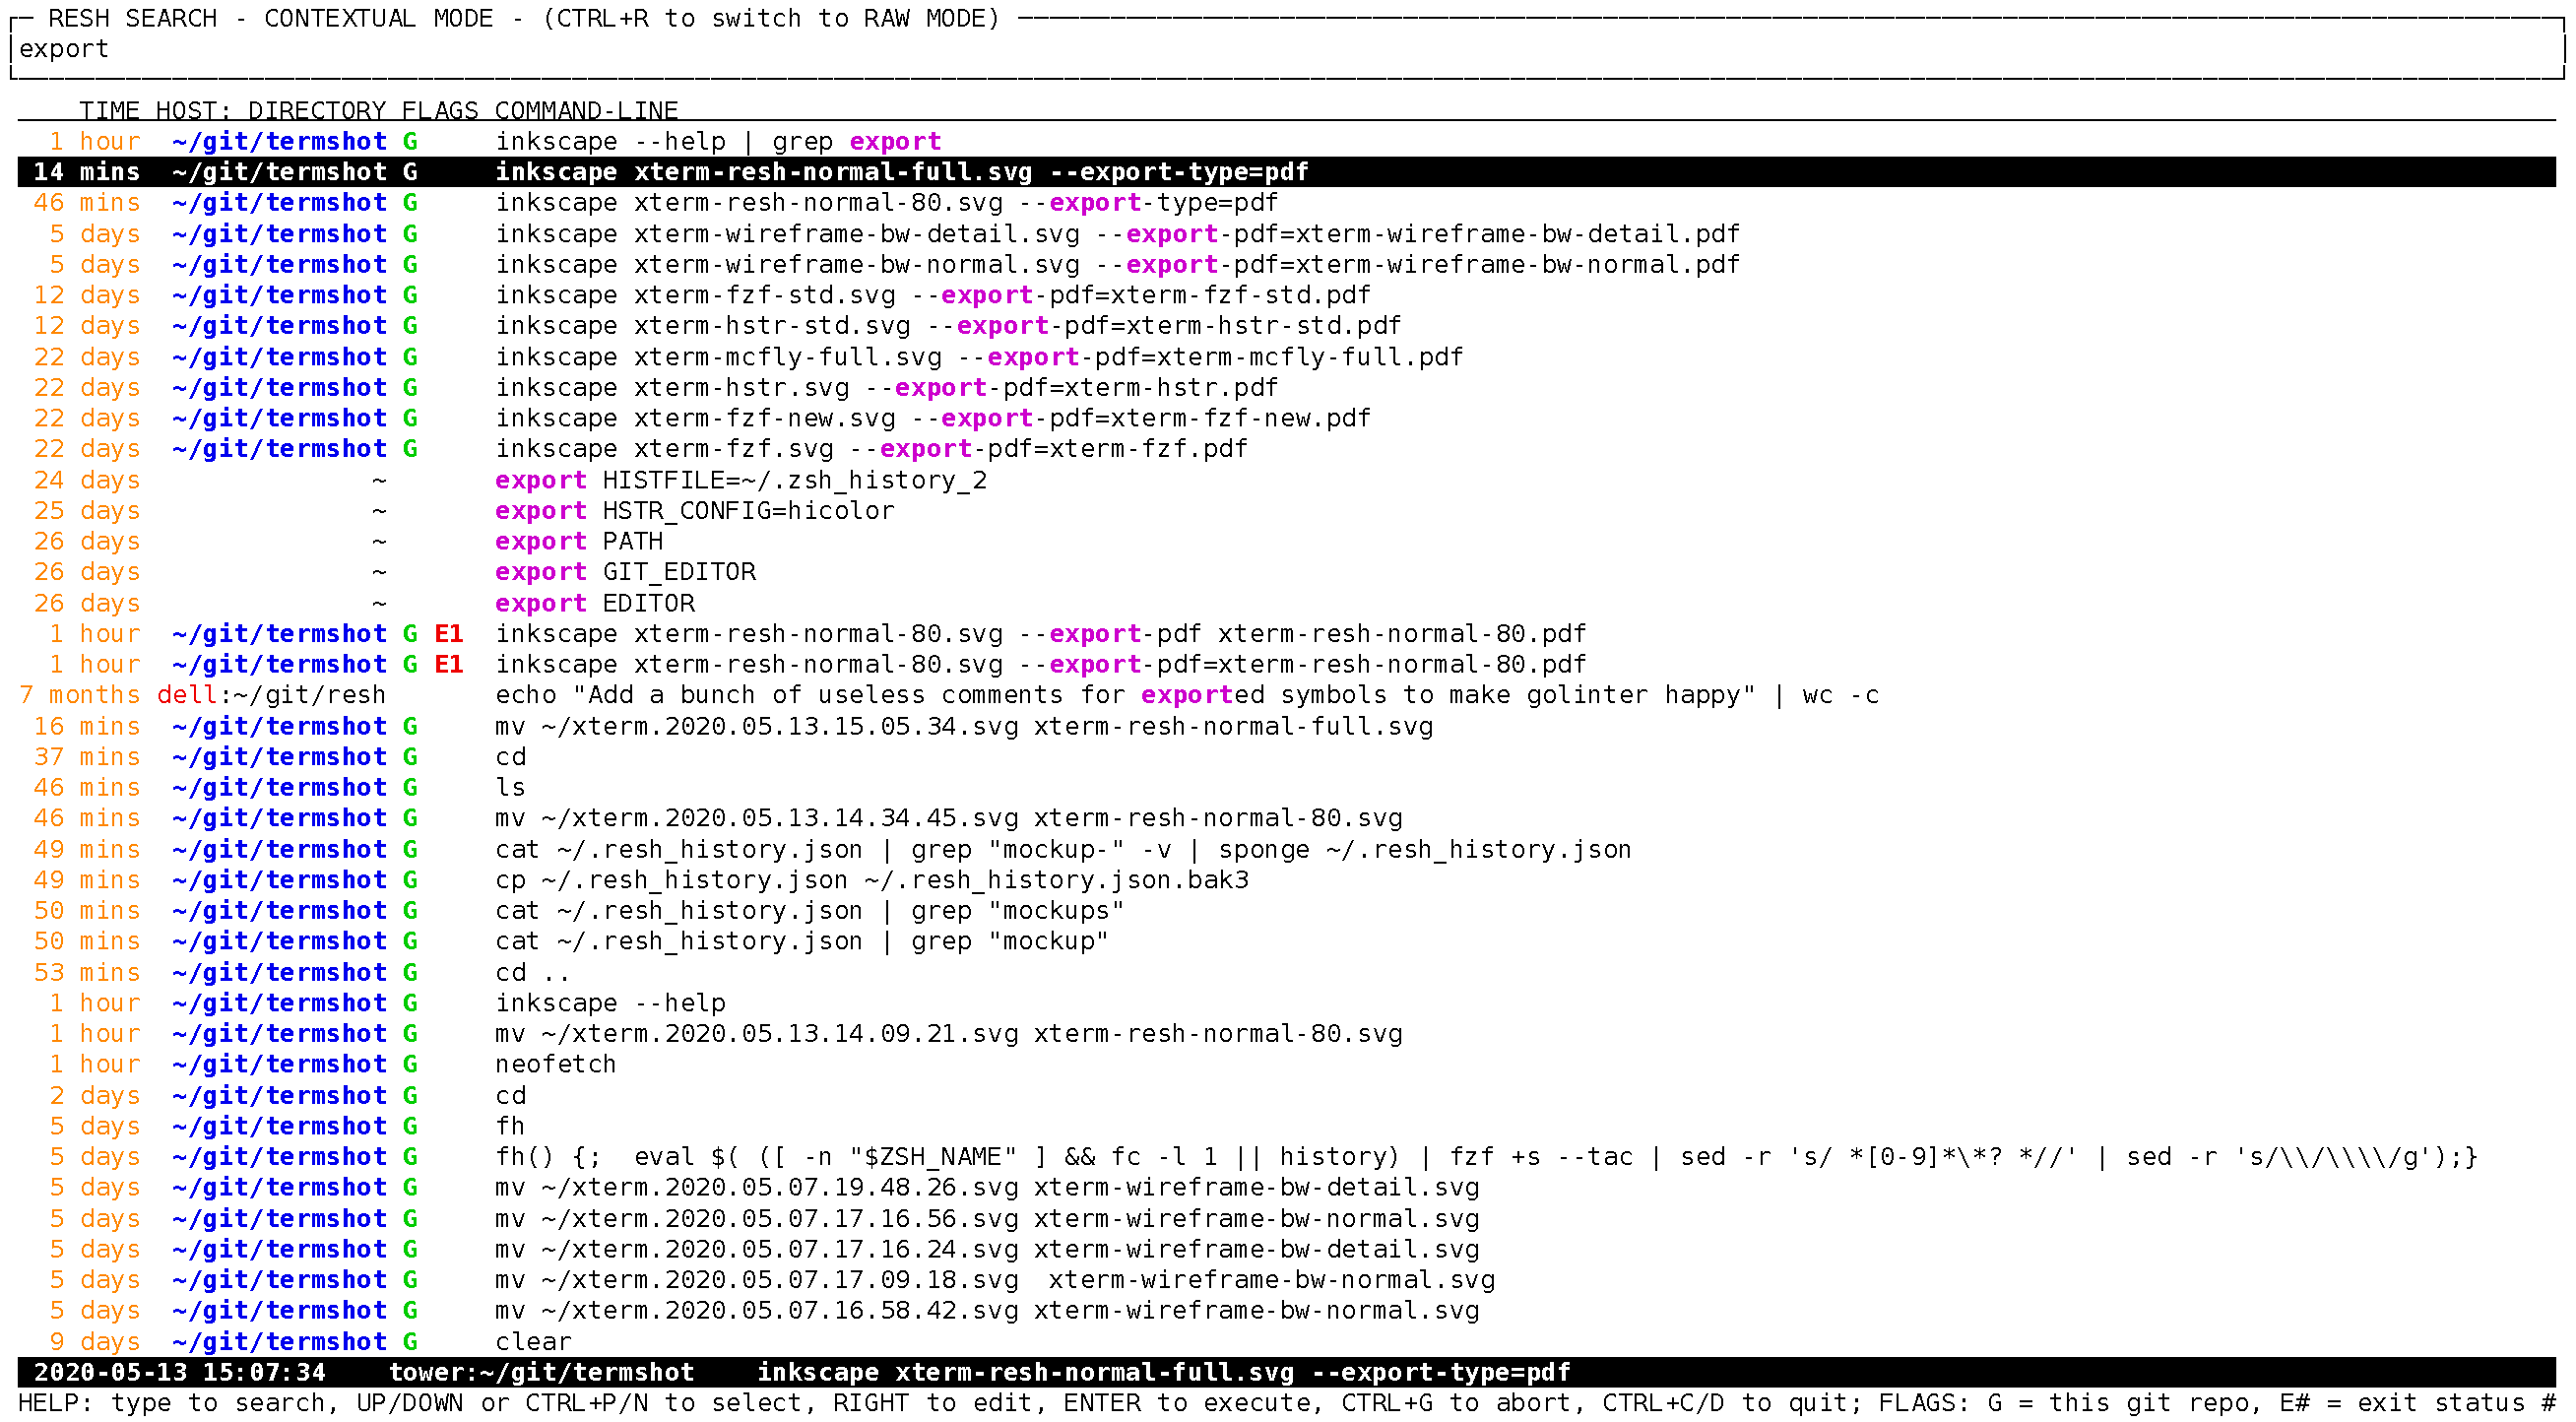
\includegraphics[angle=90,origin=c,width=0.87\linewidth]{figures/implementation/xterm-resh-normal-full.pdf}}
\caption{Screenshot of the search application in a larger terminal}
\label{xterm-resh-normal-full}
\end{figure}


\clearpage
\subsection{Calculating scores}

Earlier in figure \ref{impl-search-app-render-pipeline}, we saw calculating scores as one of the steps of the rendering process. Then we saw screenshots with search results that were searched and filtered based on scores. Now we describe how the scores are calculated.

As we explained earlier while designing, the scoring function consists of three partial scores:

\[ Score_r(q,c) = w_1 \cdot QueryScore_r(q) + w_2 \cdot ContextScore_r(c) + w_3 \cdot TimeScore_r \]


\paragraph{Query score}

To calculate the \(Query score\), we split the query into words by spaces. Then we take each word, and we match it against the history entries. For each word of the query that matches the history entry, the score is increased by \(1\). If the same word of the query matches multiple times, we add \(0.002\) to the score. 


We improve this simple matching algorithm by rewarding query words with an extra score if they match whole commands or whole arguments. We implement this in a very naive way; Any string in the command line entry that is delimited by spaces is considered a separate "word". For each query word that matches any of these "words", we increase the score by \(0.33\).

\paragraph{Context score}

Earlier, we designed \(ContextScore\) to be calculated by comparing the current context with the context of history records. This comparison should be based on four conditions shown in table \ref{tab:copy-of-score-matching-context}.

\begin{table}[h!]
\centering
\begin{tabular}{lll}
\hline \hline
Context condition & Effect \\
\hline
Directory matches & significantly increase score \\ 
Git repository matches & increase score \\ 
Non-zero exit status & decrease score \\
Host does not match & slightly decrease score \\ 
\hline \hline
\end{tabular}
\caption{Influence of different parts of context on \(ContextScore\) (table \ref{tab:score-matching-context})}
\label{tab:copy-of-score-matching-context}
\end{table}


There is an issue with these conditions; When directory matches, it is almost certain that git repository matches as well. These conditions are highly correlated.
To fix that we introduce modified conditions as shown in table \ref{tab:score-context-impl-decorrelated}.

\begin{table}[h!]
\centering
\begin{tabular}{lll}
\hline \hline
Condition name & Description \\
\hline
DIR & Directory matches \\ 
GIT & Git remote matches AND Directory does not match\\ 
ERR & Non-zero exit status \\
HOST & Host does not match \\ 
\hline \hline
\end{tabular}
\caption{Decorrelated conditions of the \(ContextScore\)}
\label{tab:score-context-impl-decorrelated}
\end{table}

To determine scores for these conditions, we took at all possible combinations, and we tried to order them. The order represents the desired behavior of \(ContextScore\); Any item in the list should get greater \(ContextScore\) than all items below it.


We found two useful ways to order the combinations. Other orders are inconsistent, or they do not match the importance of context conditions from table \ref{tab:copy-of-score-matching-context}. % For example, based on table \ref{tab:copy-of-score-matching-context}, \verb|DIR| has to be first and then we need to choose between \verb|GIT| and \verb|DIR \(\wedge\) HOST|. Once we make this choice we want to stick to it and 

\begin{multicols}{2}[]
Regular order:
\begin{itemize}
\item DIR
\item GIT
\item DIR \(\wedge\) HOST
\item GIT \(\wedge\) HOST
\item DIR \(\wedge\) ERR
\item GIT \(\wedge\) ERR
\item DIR \(\wedge\) ERR \(\wedge\) HOST 
\item GIT \(\wedge\) ERR \(\wedge\) HOST
\item (no condition)
\item HOST
\item ERR
\end{itemize}

Order with reduced penalty for non-matching host:
\begin{itemize}
\item DIR
\item DIR \(\wedge\) HOST
\item GIT
\item GIT \(\wedge\) HOST
\item DIR \(\wedge\) ERR
\item DIR \(\wedge\) ERR \(\wedge\) HOST
\item GIT \(\wedge\) ERR
\item GIT \(\wedge\) ERR \(\wedge\) HOST
\item (no condition)
\item HOST
\item ERR
\end{itemize}
\end{multicols}

Out of these two orders, we decided to use the "Regular order". This order should be better at handling situations where there are many different hosts with a lot of history. According to our previous design, each combination of conditions should result in a unique \(ContextScore\). Table \ref{tab:score-context-impl-values} shows how we assigned scores to the individual conditions in a way that produces a unique result for each combination of conditions.

\begin{table}[h!]
\centering
\begin{tabular}{lr}
\hline \hline
Condition name & Score \\
\hline
DIR & \(0.9\) \\ 
GIT & \(0.8\) \\ 
ERR & \(-0.4\) \\
HOST & \(-0.2\) \\ 
\hline \hline
\end{tabular}
\caption{Scores for conditions of \(ContextScore\)}
\label{tab:score-context-impl-values}
\end{table}

\paragraph{Time score}


To calculate the \(TimeScore\), we take the number of seconds since the epoch, and we multiply them by a coefficient to scale them to a number lower than one. The specific constant we use is $1\mathrm{e}{-10}$.

For example, the number of seconds since the epoch for 2020.05.18 at 14:05 is 
1589803500. And 1589803500 times $1\mathrm{e}{-10}$ is approximately 0.158.


\paragraph{Score weights}


Now that we covered how we implement the partial scores, we need to combine them together.
First, we want to make sure that the user can search effectively. We do not want to show results with matching context before these that match the search query. This means that a single match of a query should result in a \(QueryScore\) greater than any \(ContextScore\).

Formally, for a single word query \(q\) that matches record \(r\), for all contexts, and for all records following should hold: 

\[ w_1 \cdot QueryScore_r(q) > \max{(w_2 \cdot ContextScore)} \]

Furthermore, we do not want the contextual penalty to hide history results that match the query. We extend the previous rule to include this; For a single word query \(q\) that matches record \(r\), for all contexts, and for all records following should hold:

\[ w_1 \cdot QueryScore_r(q) + \min{(w_2 \cdot ContextScore_r)} > \max{(w_2 \cdot ContextScore)} \]

When we set \(w_2\) to \(1\) and fill in values based on definitions of the partial scores we get:

\[ w_1 \cdot 1 - 0.6 > 0.9 \]

For \(ContextScore\) weight equal to \(1\), the weight for \(QueryScore\) (\(w_1\)) needs to be greater than \(1.5\). This way a single query match has enough influence compared to the context.

Now we have determined all weights except for \(TimeScore\) weight. We only want \(TimeScore\) to influence the order when everything else is equivalent. To do this we set the weight for \(TimeScore\) (\(w_3\)) to $1\mathrm{e}{-3}$.

Table \ref{tab:score-weights-ranges} shows weights and ranges for all partial scores. The maximal \(TimeScore\) is 0.9 for all dates up to year 2255. The maximal \(QueryScore\) is 1.37 per each word of the query for up to 20 consecutive matches. 

% Theoretically, the maximal value for \(QueryScore\) is unlimited because there can be any number of consecutive matches. However, realistically, we will rarely have more than a few consecutive matches; 

\begin{table}[h!]
\centering
\begin{tabular}{lrrr}
\hline \hline
Partial score & Weight & Minimal value & Maximal value \\
\hline
$QueryScore$ & 1.51 & 0 & 1.37 per word of query  \\ 
$ContextScore$ & 1 & -0.6 & 0.9 \\ 
$TimeScore$ & $1\mathrm{e}{-3}$ & 0 & 0.9 \\
\hline \hline
\end{tabular}
\caption{Weights and ranges for partial scores}
\label{tab:score-weights-ranges}
\end{table}

\newpage
\section{Daemon}

So far, we covered the implementation of the search application and the necessary shell integration. Now we describe how we implement the daemon.

%\subsection{Overview}

As you can see in figure \ref{impl-daemon-channels}, the daemon consists of four parts that communicate asynchronously using Go channels\cite{lib-go-channels}. We use standard Go HTTP server\cite{lib-go-http} to listen for requests. 

The history collector uses \verb|/record| request to send history records to the daemon. The search application uses \verb|/dump| request to get all history records. And the \verb|/recall| request is used by the arrow key handler to get command line entries from the daemon. 

All of the requests use JSON as a data exchange format. Conveniently, history records are also saved to storage as JSON. 

\redtext{Link to JSON description of JSON}

\begin{figure}
\centering
\tmpframe{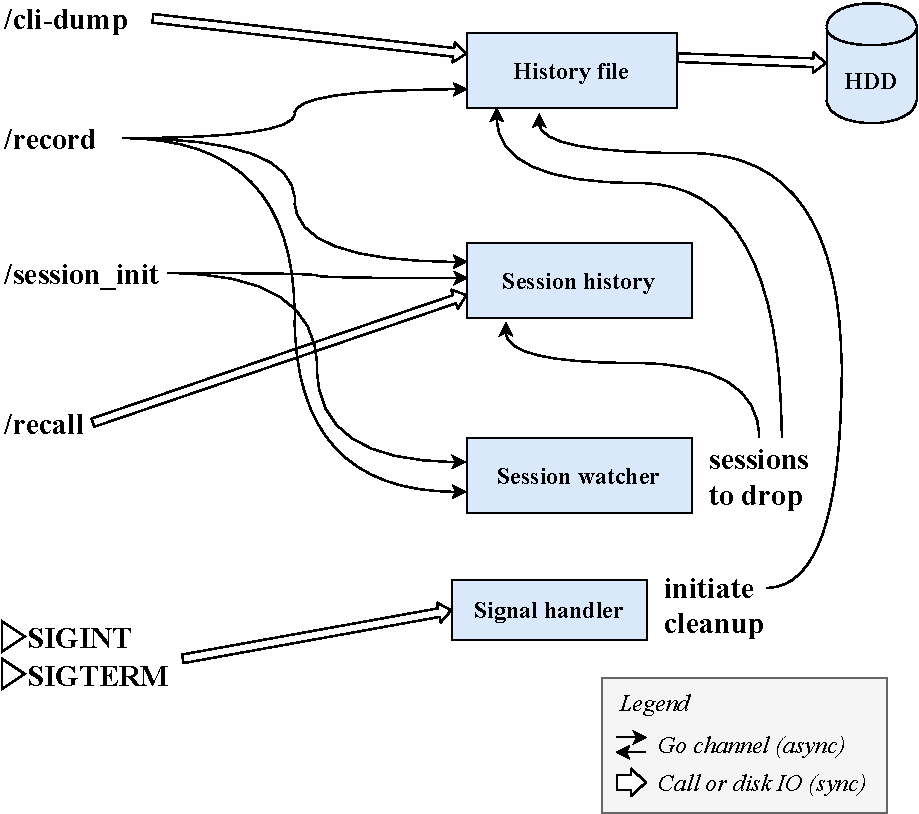
\includegraphics[width=\linewidth]{figures/implementation/thesis-impl-daemon-channels.pdf}}
\caption{Schema of internal daemon structure and communication}
\label{impl-daemon-channels}
\end{figure}

\subsection{History file module}

The history file module is responsible for all communication with a storage device. It reads history records from storage when it starts up. And it also writes history records to storage.

Earlier, we explained that the history collector is activated before and after each executed command line. This means that the history record is sent to the daemon in two parts. The history file module is responsible for merging the two parts into a single history record. 

When the search application sends \verb|/dump| request, the history file module responds with all history records. 

% standard shell history

\subsection{Session history module}

The session history module holds the history for active sessions. It receives history records from \verb|/record| requests and appends them to history for the matching session.
These session history structures only exist in memory.

The session history module responds to \verb|/recall| requests from the arrow key handler. The history for the session is retrieved, and an appropriate history entry is returned. 

\subsection{Session watcher module}

The session watcher module is responsible for keeping track of which sessions are no longer active. Any history records sent to the daemon using \verb|/record| requests are also sent to the session watcher module. 

Whenever a new history record is received, the session watched module looks at the session it belongs to. If it is not already watching this session, it starts periodically checking if the session is still active. Specifically, we check if the process with the PID of the session is still running.

Once a session becomes inactive, the session watcher module notifies the session history and the history file modules. These modules delete appropriate structures from memory.

\subsection{Signal handler module}

The signal handler module is responsible for shutting down the daemon when it receives \verb|SIGINT| or \verb|SIGTERM| signal. First, it notifies the history file module to write out all pending history records to the storage device. Once this is done, or a timeout is exceeded, the signal handler module shuts down the whole daemon.


\section{Installation, updates, and configuration}

Writing the software is just the first part of the process. Releasing it and getting it to your users is equally important. In this section, we describe how we build the project and how users can install it.

\subsection{Releasing and building the project}

Our project is hosted on GitHub\cite{resh-github-homepage}. We have set up a CI pipeline to build binaries of the project for every tag we push to the repository. Specifically, we use GitHub Actions\cite{github-actions} and Goreleaser\cite{tools-goreleaser}.

When the CI pipeline builds the binaries, it creates a new release on the release page\cite{resh-github-releases}. The built binaries are available there. 

\subsection{Installation and updates}

The project can be installed by running a simple installation script.
First, the script checks the operating system and the CPU architecture of the device. Based on that, an archive with appropriate binaries is downloaded. Then, an integrity check is performed, and the archive is extracted. 

After extracting the archive, we check versions of Bash and Zsh, make directories, and copy files. We also append a few lines to users dotfiles to set up the shell integration. Finally, we show some onboarding information to the user.

The project has almost no dependencies. There are only a few very standard utilities required for installation. The binaries are statically linked, so they do not depend on any system libraries.

The project can be updated at any time by running \verb|reshctl update|. This checks if there is a new version of the project available and installs it.

\subsection{Configuration and control}

Our project comes with a configuration command \verb|reshctl|. Besides other things, this command can be used to enable and disable key bindings. 

Tab completions for \verb|reshctl| are set up during installation. There is a help (\verb|-h|/\verb|--help|) option available with descriptions for individual subcommands. To make it easy to provide all this, we use a library\cite{lib-go-cobra} for creating command line interfaces.



\chapter{Evaluation and Testing}

In this chapter, we evaluate and test the implemented history system to find out how useful it is.

First, we explain what does it mean for a system of a tool to be useful. Plus we point out the specifics of estimating the usefulness of history systems.

Second, we use a few real life scenarios to show the advantages of our search application in practice. Using these scenarios we compare different methods to search for and retrieve entries from shell history.

Third, we introduce metrics to quantitatively evaluate our history system. Then, we use the metrics to compare our search application with another state-of-the-art history tool.

Fourth, we describe how we incrementally improve the system since the initial release. The community of existing users makes it possible to get impressions, ideas, and feedback. 

Finally, we show additional workflows that are possible to fulfill using our search application. 

\section{Usefulness of history tools}

The goal of this work is to design and create a history system that is useful. 
We want people to use the tool because it both solves their workflows and it is easy and pleasant to use.

The usefulness of the system is determined by its utility and its usability.\cite{nielsen2012usability} Utility is a quality attribute of the system that assesses if the system provides the features that users need.\cite{nielsen2012usability} Usability refers to how easy and pleasant are the features to use. Any useful system needs to have both good utility and usability.

In following sections we describe what utility and usability means for history tools specifically.

\subsection{Utility}

History systems should make it cheaper, in terms of mechanical and cognitive activity, to retrieve history entries than to type them again.\cite{greenberg1993computer}

Retrieving command line entries from history saves us typing. Even small savings in typed characters make a difference because typing is an error-prone activity; A significant amount of time is usually spent detecting and fixing errors. According to \cite{whiteside1982people}, typing only accounts for about a half of all key strokes during text editing. 

%"Command line entry involves not only typing the final correct characters, but also the time it takes to detect and correct typing errors. Actual character savings are likely double the theoretical ones" \cite{whiteside1982people}

Before typing the command line entry, the user has to think of what to type. In many cases, this might be more difficult than the act of typing out the command line entry.   

%Generally, recognizing and selecting and activity is considered easier than recalling it or regenerating it. \cite{greenberg1993computer}

To evaluate the utility of our history system we use metrics that are based on how many characters users retrieve from history and how much information is required for a successful retrieval.

\subsection{Usability}

Usability represents how easy to use the interface of the system is. Usability can be broken down to five following quality components: Learnability, Efficiency, Memorability, Errors, and Satisfaction.\cite{nielsen2012usability}

%\begin{itemize}
%    \item Learnability
%    \item Efficiency
%    \item Memorability
%    \item Errors
%    \item Satisfaction
%\end{itemize}

Learnability assesses how easily can users complete basic task when they use the system for the first time. For example, non-standard key bindings that are not shown on the screen could make the interface difficult to use.

Efficiency means how quickly can users achieve their goals once they already know how to use the system. If the design requires users to complete too many steps to accomplish their goal it will slow them down. 

Memorability represents if the users can proficiently use the system after they did not use it for a while. 

We also want to know how many errors people make while using the system. Does the design make it easy to recover from errors? For instance, if there would be no way to revert ones actions the users might learn to use the system slowly and carefully. 

Satisfaction assesses if it is pleasant to use the system. For example, system that unpredictably fails will likely cause its users to distrust it. Users probably will not enjoy using a system they find unreliable. 

%Learnability: How easy is it for users to accomplish basic tasks the first time they encounter the design?
%Efficiency: Once users have learned the design, how quickly can they perform tasks?
%Memorability: When users return to the design after a period of not using it, how easily can they reestablish proficiency?
%Errors: How many errors do users make, how severe are these errors, and how easily can they recover from the errors?
%Satisfaction: How pleasant is it to use the design?

\subsection{Issues with testing history tools}

Ideally, we would want to perform usability testing with users; This would help us to find usability issues of the system and estimate its overall usability.

When conducting usability testing we want to see users perform real tasks using the system. It is necessary to prepare testing scenarios for users to follow during the testing session.

However, history tools cannot be tested as easily as other applications or websites.
Unlike with other applications, scenarios for our history search application are heavily dependent on the personal workflows of the specific user and his history.


We would need to prepare personalised scenarios for individual users based on their shell history and their usage of the history mechanisms.
This is possible but it proved to be too time consuming for us to use in this work.

We released this project a while ago and we iteratively improve it. Because of that we got a lot of feedback and many chances interview our users. We also collected some shell history and usage data from our users. We use this data to demonstrate the usefulness of our solution.

\section{Evaluating real life scenarios}\label{test-real-life-scenarios}

In this section, we compare our history searching with other history tools based real life scenarios. We have collected shell history with usage from some of our users and chose specific situations to showcase the advantages of using our history search application.

We found situations when people have used either Hstr\cite{toolshstr} or our search application to retrieve history entries. These match the following workflows from our previous analysis:

\begin{itemize}
\item Searching with limited knowledge (section \ref{workflow-search-w-limited-knowledge})
\item Searching with implicit context (section \ref{workflow-search-w-implicit-context})
\end{itemize}
We took the shell history available at the time and fed it into three different history tools. The tools we test are standard reverse search, Hstr, and our search application. Now, we compare how difficult it is to retrieve the desired history entry using these three history tools.

\redtext{Consider adding one more scenario}
\subsection{Searching with limited knowledge}

In this first real life scenario, the user is trying to retrieve following history entry: 

\begin{verbatim}
ansible-galaxy install -r requirements.yml -p roles
\end{verbatim}

%\verb|/Users/vit.listik/git/szn/laas/ansible-etcd|

\paragraph{Reverse search}
If the user used reverse search and typed \verb|ansible| as a query, the desired history entry would be twenty results away. As we described earlier in section  \ref{workflow-search-w-implicit-context}, pressing \verb|CTRL-R| twenty times while reading the results one by one is quite inefficient.

Instead of using \verb|ansible| as a query and going through many results, the user could use a more specific query. Using \verb|ansible-g| as a query returns the desired history entry as the first result. In this case, however, the user has to remember more information about the history entry.

\paragraph{Hstr}
Now, we look at how the user could use Hstr to retrieve the same history entry.
Typing \verb|ansible| returns the history entry on twentieth position on the page. Unlike with the reverse search, the user could fairly quickly scan the page and select the desired history. 

However, it could be faster to extend the query to further filter the results. Unlike with the reverse search, the user can use any part of the command line entry as a query because Hstr breaks the query down to separate words. Extending the query to \verb|ansible ins| returns the desired entry as the first result.

% Hstr requires less knowledge and less typing than reverse search. Plus selecting a twentieth result in Hstr is realistic unlike in reverese search.

\paragraph{Our contextual search application}
Finally, we compare how our search application performs compared to the other two options.
After the user opens the search application the desired result is already in the third position. The user does not even have to specify a query because the search application returned the history entry based on the current context.

Typing \verb|ans| as a query brings the desired history entry to the first position. As we can see, our solution requires less knowledge and less typing to retrieve the desired history entry than both Hstr and reverse search. 

\subsection{Searching with implicit context}

In this second scenario, the user wants to retrieve the following history entry:

\begin{verbatim}
ansible-playbook infra_os_deploy.yml -i inventory_example.ini \
-b -u debian -D
\end{verbatim}

%\verb|~/git/szn/laas/ansible-playbooks|

\paragraph{Reverse search} 
First, we look at how the user could use the reverse search to retrieve the desired history entry.
Using \verb|ansible-playbook| as a query returns the history entry as thirty-first result. This is practically unusable. Plus this query is very hard to extend.

The user could chose to delete the query and use a different one. Coming up with a usable query is hard in this case; For example, typing \verb|inventory| or \verb|debian| returns the history entry as second and third result respectively. In contrast, using \verb|infra| or \verb|deploy| leaves the entry well beyond the reach of the user. 

\paragraph{Hstr}
Second, we describe how Hstr can be used to retrieve the previously mentioned history entry.
Typing \verb|ansible| does not return the desired history entry. However, the user can quite easily extend the query to \verb|ansible inf| which returns the history entry as a first result. 

We can see how the ability use multi-word queries makes it much easier to use Hstr than reverse search.

\paragraph{Our contextual search application}

Third, we compare our search application with both previous methods. 
When the user launches the application, he can already see the desired history entry as the eight result on the page. This is possible because the current context matches the context of the desired history entry. 

As before, typing \verb|ans| as a query brings the desired history entry to the very first position on the page. 

In situations like this one, our search application makes it very easy to retrieve the desired history entry. Hstr provides an reasonable to retrieve the entry but using context gives advantage to our solution. Reverse search is nearly impossible to use in this scenario.


\section{Introducing metrics}

In previous section, we demonstrated the advantages of using the contextual search application using specific situations we found in shell history of our users. We saw how reverse search can be very ineffective. In contrast both Hstr and our search application performed adequately.

Here, we introduce metrics we will use to evaluate the utility of our search application. We will later use these metrics to compare our search application with Hstr. 

\subsection{Number of saved characters}

The first metric is the number of saved characters. Retrieving longer history entries from history saves more work to the user. Longer history entries take more effort to type. Remembering longer history entries is also likely more difficult than remembering shorter ones. 

% Since we compare two similar history tools we assume that the number of key strokes needed to select the history entry is similar once it has been found. Because of that we are not subtracting the key strokes needed for selection inside the history search applications.

\subsection{Amount of required knowledge}\label{knowledge-tokens}

The second metric represents the amount of knowledge the user needs to retrieve the history entry. We measure the amount of required knowledge in the unit of "knowledge tokens".

Knowledge tokens are substrings of the command line entry that consist of alphanumerical characters and are at least four characters long. We chose this definition of a knowledge token because it matches the type of information people usually remember and use for searching. We observed this behavior in our users. 

\redtext{Check "newpage"}
\newpage 
For example, imagine that you are searching for the following history entry:
\begin{verbatim}
curl -O -L https://api.github.com/repos/curusarn/resh/releases  
\end{verbatim}

You would probably use something like \verb|curl github| as a query. The longer chunks of letters represent meaningful information while symbols are repetitive noise.

\subsection{Position on the screen}

Last metric we use is the position of the history entry on the screen. Both of the history searching tools we are testing show a screen full of results. There is a significant difference between returning the history entry as the first result compared to displaying it near the bottom of the screen. It takes extra time to scan the screen and notice the result. Plus, even the act of navigating and selecting results near bottom of the screen takes additional effort.

\section{Applying metrics}

In this section, we apply the previously introduced metrics to compare the performance of Hstr and our search application. We simulate searches based on collected usage data and then we use the metrics to compare and evaluate the results. 

\subsection{Collected data}

We have collected shell history and usage data from a few of our users. Out of these users there is a single user that was previously using Hstr and switched to our history search application. We use the data from this user to compare the utility of these two history applications.

During five months of collecting the data, this user has executed 12 thousand command line entries. He has successfully used Hstr 121 times and our history search application 69 times. 

For each time the user has searched his history we know what history entry the user retrieved and executed. We also know when the event happened. This means that we can take the shell history that was available at the time and feed it into Hstr and our search application. This way we can see what results would these history tools return at that time. We can compare how difficult would it be to retrieve the desired history entry in either of the history tools. 

We should note that Hstr normally uses standard shell history for searching. Standard shell history can be missing history entries. This can be caused by upper history size limit and losing history from simultaneous terminal sessions.

When we compare our history search application with Hstr we are providing our collected history to Hstr. This means that in following tests we share the advantage of having complete timestamped history without missing history entries with Hstr. In reality, we would expect the performance of Hstr to degrade because of the missing history entries.

\subsection{Simulating history searching}

To evaluate the history tools we simulate the successful searches performed by the user. Then we use previously introduced metrics to compare the utility of these history tools.

When simulating the searches, we iterate over all situations when the user searched his history\footnote{Actually, we skip searches performed before the first one thousand history entries. We do this to not perform searches on almost empty history. We can still observe some minor warm up effect but it does not skew the results.}. With each simulated searches we are essentially asking questions such as:

\begin{itemize}
    \item Does this history entry show up in \textbf{first 20 results} if we use \textbf{no query}?
    \item Does this history entry show up in \textbf{first 20 results} when we use \textbf{one word as a query}?
    \item Does this history entry show up as \textbf{the first result} when we use \textbf{two words as a query}?
\end{itemize}
The process of simulating a single search is following:

\begin{enumerate}
    \item Take all shell history available at the time of the search
    \item Feed the history into either Hstr or our search application
    \item Process the desired history entry into knowledge tokens (described in section \ref{knowledge-tokens})
    \item Shuffle the knowledge tokens\footnote{The sequential order is a bad representation of how people choose search queries in history tools. We deterministically shuffle the list of knowledge tokens by moving every odd token to the end of the token list.}
    \item Take \(N\) of the knowledge tokens and use them as a query
    \item Find the desired history entry in the list of results and return its position as \(M\)
\end{enumerate}

Simulating a single search tells us that a specific history entry shows up on \(Mth\) position when we use \(N\) words as a query.


\subsection{Comparing our search application with Hstr}

We have just explained how we simulate searches that were performed by the user. We can compare how different history searching tools perform by simulating the searches. 

In the usage data we are using, the user has originally used Hstr for a period of time and at some point he started using our search application. These two parts of the usage data differ because people use different tools differently. We take these two parts of the usage data and separately test how both of the history tools would perform. 

Essentially, we test how our search application performs in situation when the user originally used Hstr. And conversely, we test how Hstr performs in situations when the user originally used our search application.

\paragraph{Achievable searches as a function of knowledge}

The first thing we want to find out is how many searches are achievable and how much the user has to remember to achieve them. We only count the search as achievable if the desired history entry is returned in the first 20 results.\footnote{The first twenty results represents an amount of lines that fits even into small terminals.} 

Figure \ref{eval-metrics-plot-cmds} shows us the percentage of searches that we could achieve if we only used a limited number of knowledge tokens (words) as a query. 

The figure \ref{eval-metrics-plot-cmds} is split into two parts; The left part shows situations when the user originally used Hstr. The right part show situations when the user originally used our search application. As we can see, both history tools perform very similarly for original usage of Hstr. However, our search application performs significantly better in situations when it was originally used. 

Using our search application, the user can successfully complete 48.5\% searches with zero knowledge. In comparison, Hstr only shows the correct history entry with no query in 26.8\% of searches. 
This means that if the user switched back to Hstr, he would have to start typing queries for about a half of searches that previously worked without any query.


When we use more knowledge tokens as a query the differences between Hstr and our search application get insignificant. This is expected, our solution is designed to prioritize query over context. As we add words to the query, the \(QueryScore\) dominates the \(ContextScore\) and our search application behaves more and more as non-contextual search. This is essential because it gives users control over the search and enables them to find what they need.
\redtext{ADD a plot to show how QueryScore and ContextScore mix}

\begin{figure}[h!]
\centering
\tmpframe{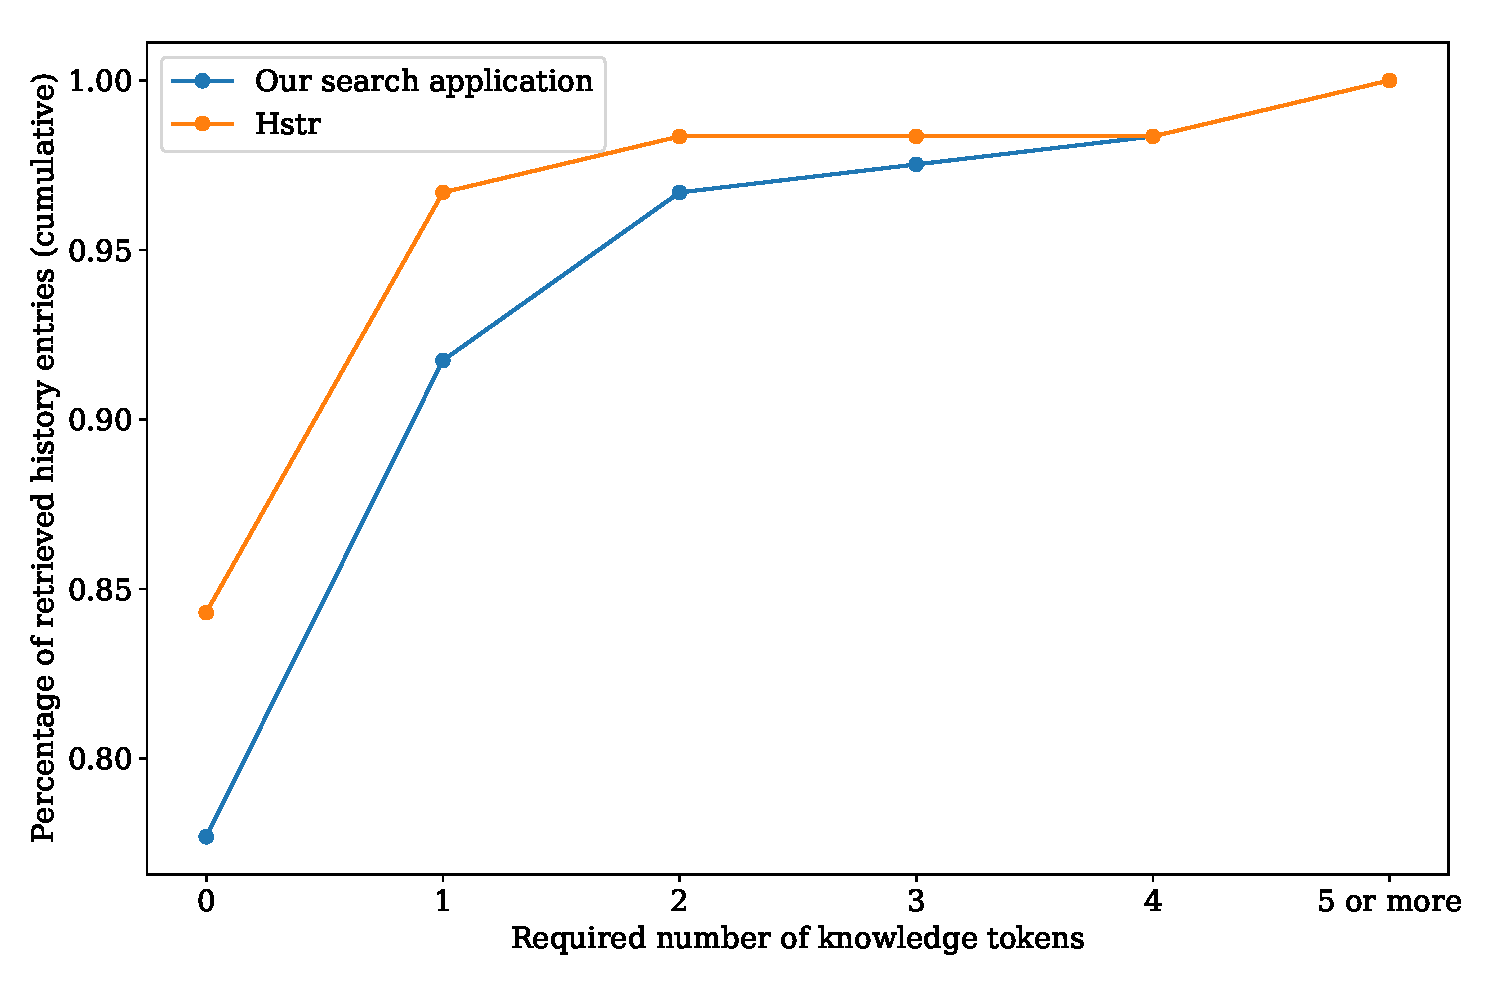
\includegraphics[width=0.5\linewidth]{figures/testing/testing-metrics-cmds-hstr.pdf}}\hfill
\tmpframe{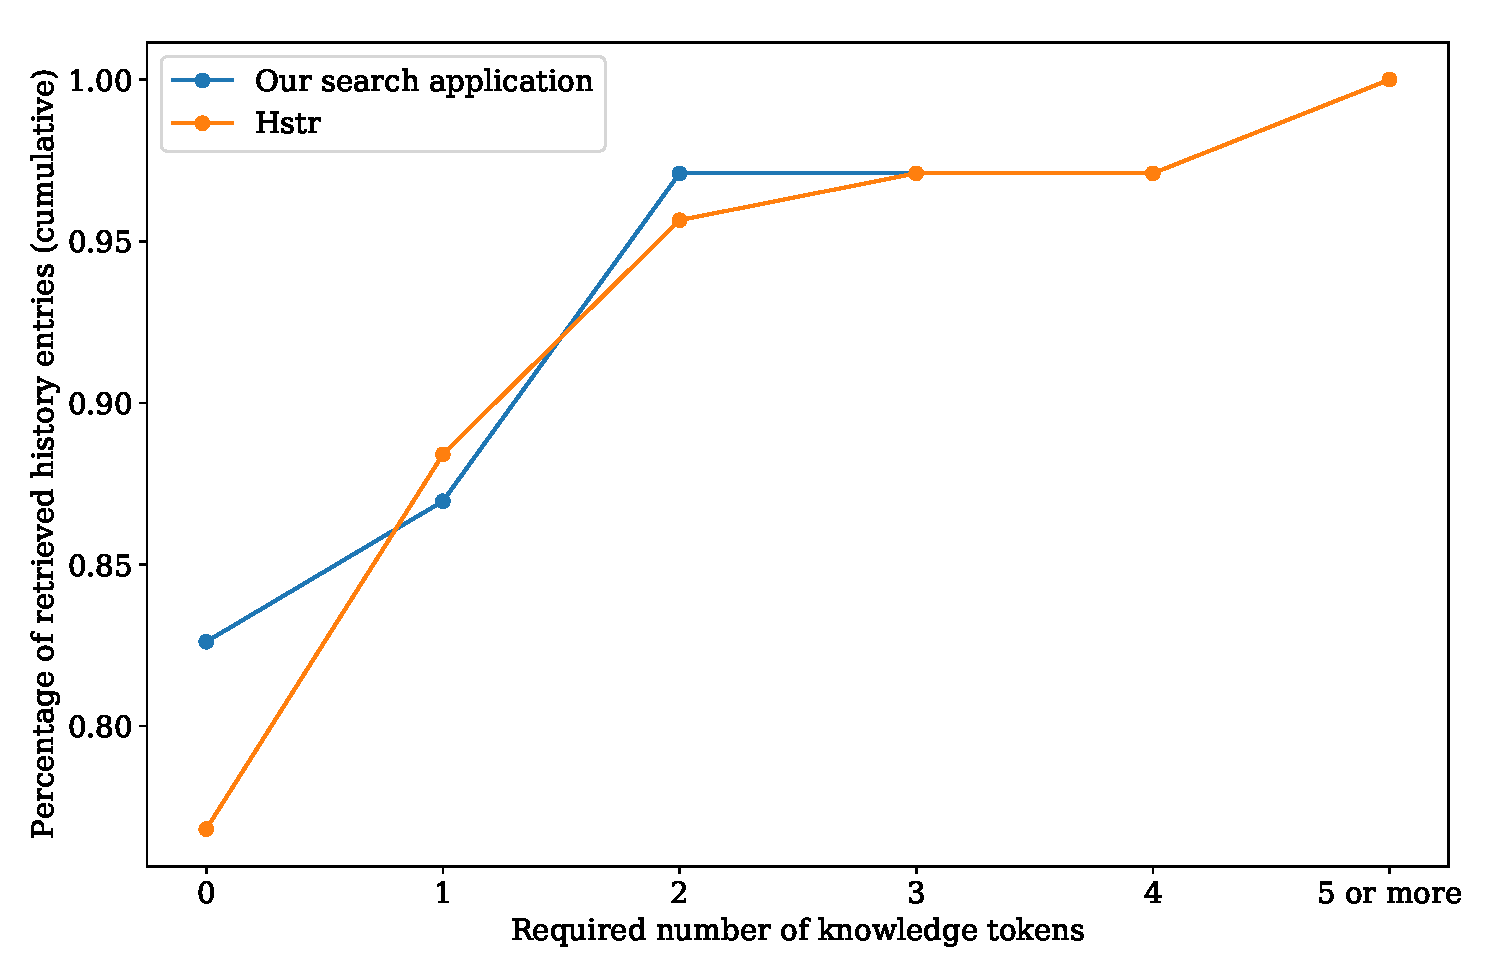
\includegraphics[width=0.5\linewidth]{figures/testing/testing-metrics-cmds-resh.pdf}}
\caption{Achievable searches as a function of knowledge (more is better)}
\small{Originally usage of Hstr (left) and usage of our search application (right)}
%\caption{Percentage of achievable searches (Originally performed using Hstr)}
\label{eval-metrics-plot-cmds}
\end{figure}

\begin{figure}[h!]
\centering
\tmpframe{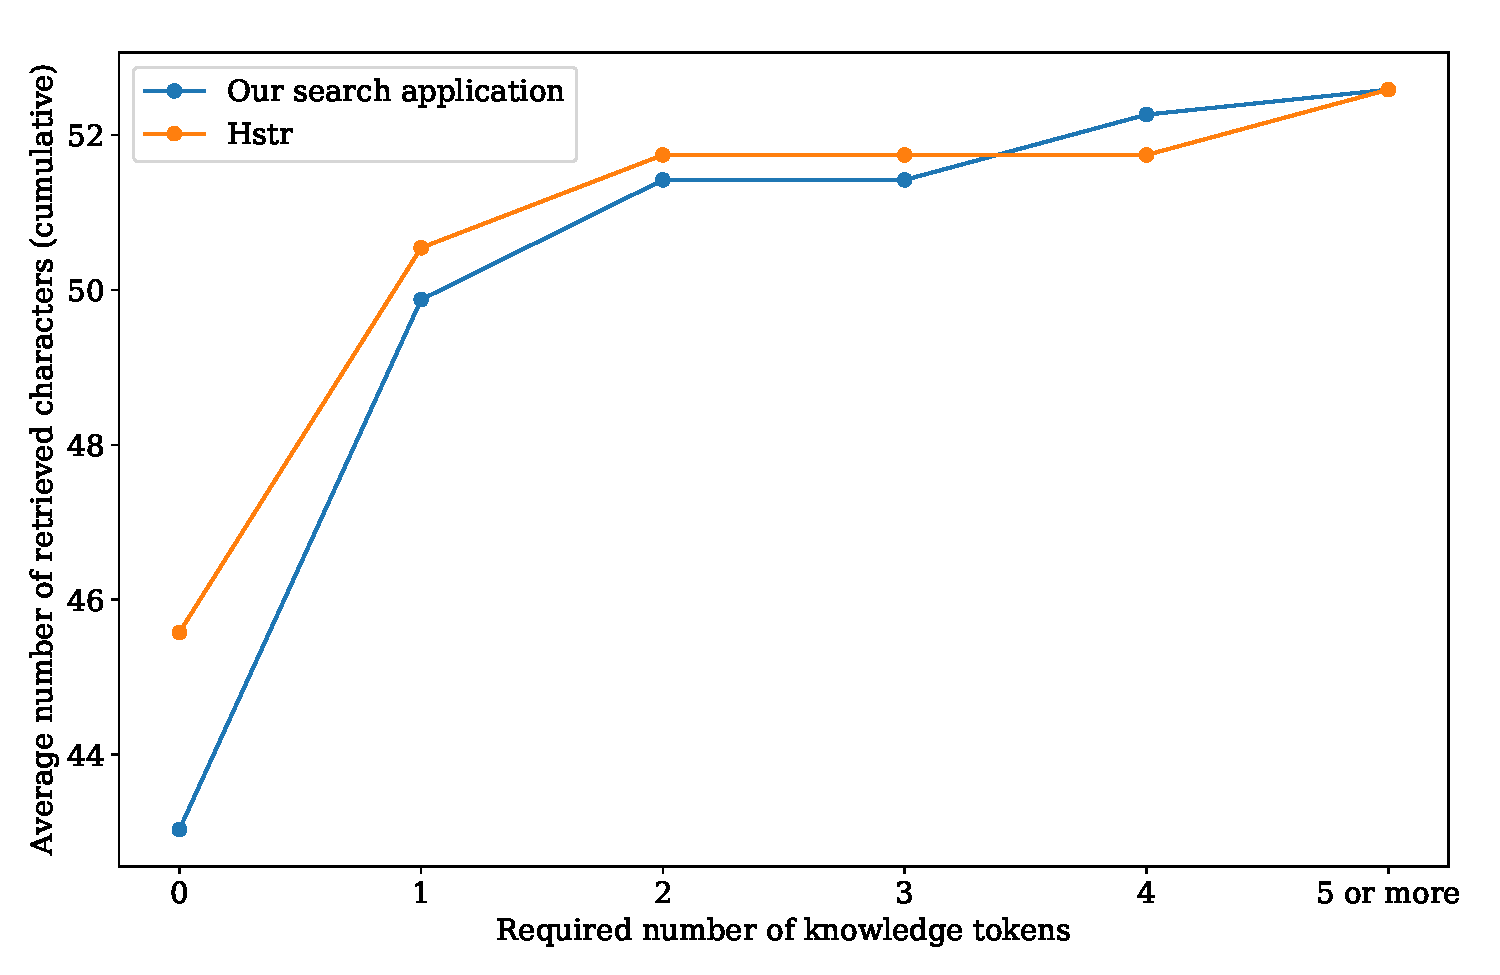
\includegraphics[width=0.5\linewidth]{figures/testing/testing-metrics-chars-hstr.pdf}}\hfill
\tmpframe{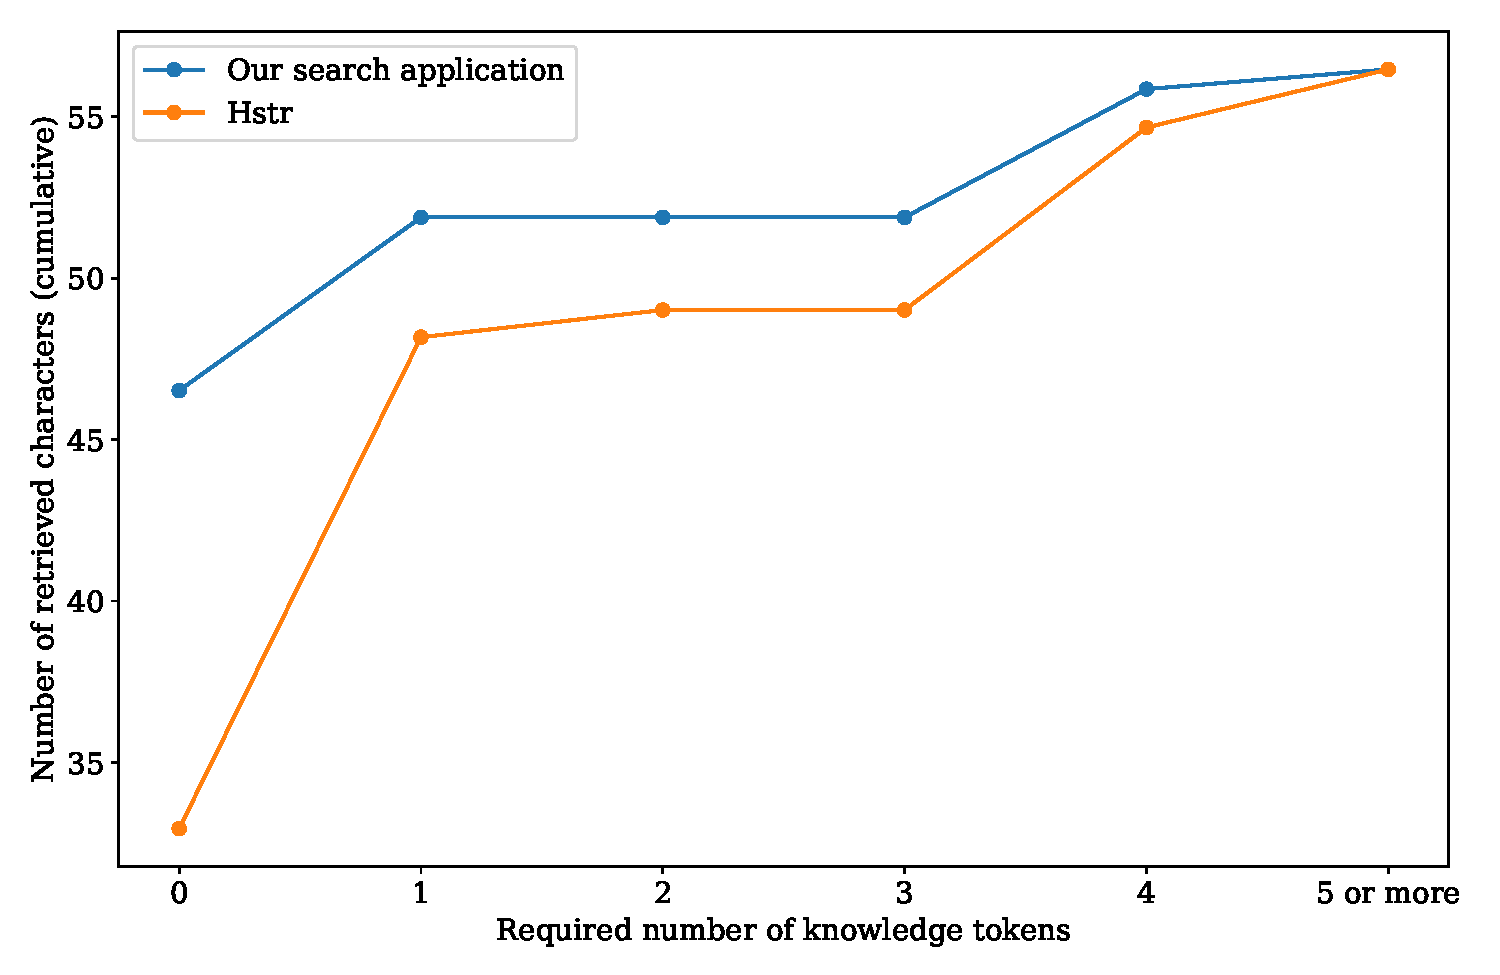
\includegraphics[width=0.5\linewidth]{figures/testing/testing-metrics-chars-resh.pdf}}
\caption{Avg. saved characters as a function of knowledge (more is better)}
\small{Originally usage of Hstr (left) and usage of our search application (right)}
\label{eval-metrics-plot-chars}
\end{figure}


\paragraph{Average saved characters as a function of knowledge}

Again, we are looking at how many searches are achievable for a limited number of knowledge tokens. However, we are also taking the length of the retrieved history entries into account. Essentially, searches that retrieve longer entries are worth more than shorter ones.

% In the previous section, each search was worth the same; Here, the searches retrieving longer history entries are worth more then ones retrieving short entries.

In figure \ref{eval-metrics-plot-chars}, we can observe many of the same characteristics as we saw in previous figure \ref{eval-metrics-plot-cmds}. Both history tools perform similarly in situations when the user originally used Hstr (left part of figure \ref{eval-metrics-plot-chars}). Our search application performs significantly better in situation when it was originally used (right part of figure \ref{eval-metrics-plot-chars}). 

When we compare figure \ref{eval-metrics-plot-cmds} with \ref{eval-metrics-plot-chars}, we can see that the difference between our solution and  Hstr is more substantial when we take retrieved characters into account. 

Our application not only achieves more searches with limited knowledge; It also returns longer history results on average.

The fact that contextual history yields longer history entries is not surprising; It matches findings from previous research\cite{greenberg1993computer} where directory sensitive history returned longer history entries then simple recency-based history. More specific history entries generally tend to be longer and generic and common command line entries tend to be shorter. 


\subsection{Position of results on the screen}

We have shown the difference between situations when user originally used Hstr and when he used our search application. We have also explained why our application starts behaving similarly to Hstr as we increase the number of words we use as a query.

The main difference in performance between Hstr and our search application happens when we only search using little or no knowledge. Because of that we further explore how the two history tools perform when searching with limited knowledge.

In this section, we are testing how many searches we can complete and how close to the top of the screen retrieved results show up. 

\paragraph{Achievable searches with zero knowledge}

Here, we want to find out how many searches are achievable if we only accept results from a given number of top positions. We are not using any query because we need to find out how well the search tools works when the user remembers nothing.

Figure \ref{eval-metrics-plot-dist-0-cmds} shows the percentage of searches that we could achieve if we only accepted results from limited number of top positions on the screen. In other words, how many searches can we complete if we are only accepting results from e.g. first 10 returned results.

We can see that the performance of both history tools is similar in situations when the user originally used Hstr (left part of figure \ref{eval-metrics-plot-dist-0-cmds}). We will see this in all figures in this section. To not repeat ourselves, we are not going to mention it anymore.

As shown by the right part of figure \ref{eval-metrics-plot-dist-0-cmds}, Hstr and our solution performs similarly if we only accept results from first nine positions (or less). If we accept results further down the screen our solution is able complete significantly more searches than Hstr.

\redtext{Explain why we end at 20 - the size of views ... ADD plot for longer X with lines for significant screen sizes}
\redtext{Con}

Figure \ref{eval-metrics-plot-dist-0-chars} is very similar to figure \ref{eval-metrics-plot-dist-0-cmds}. It shows average saved characters instead of percentage of searches. All of the previous observations still hold. The performance differences between our solution and Hstr are more pronounced. 


\begin{figure}
\centering
\tmpframe{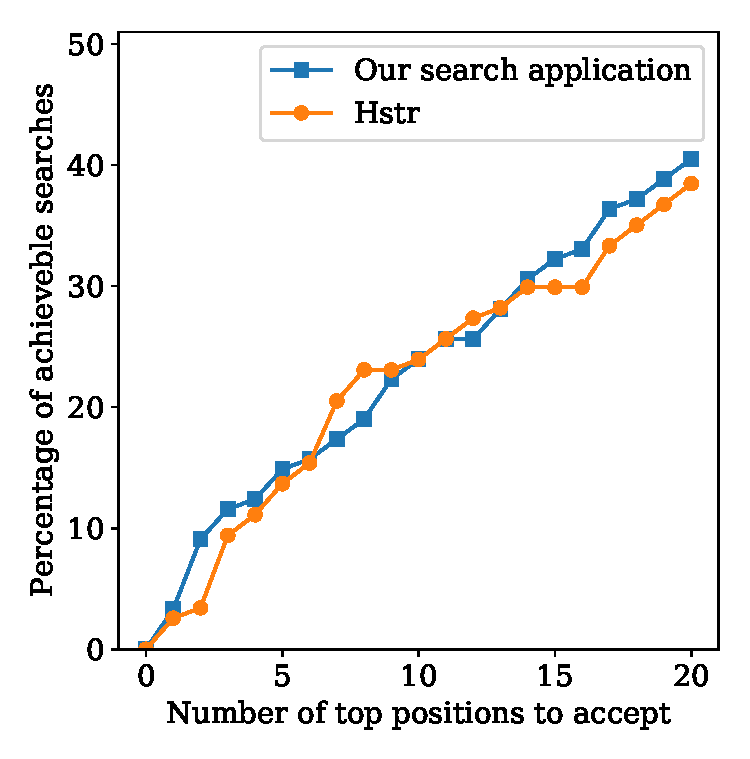
\includegraphics[width=0.5\linewidth]{figures/testing/testing-metrics-dist-0-cmds-hstr.pdf}}\hfill
\tmpframe{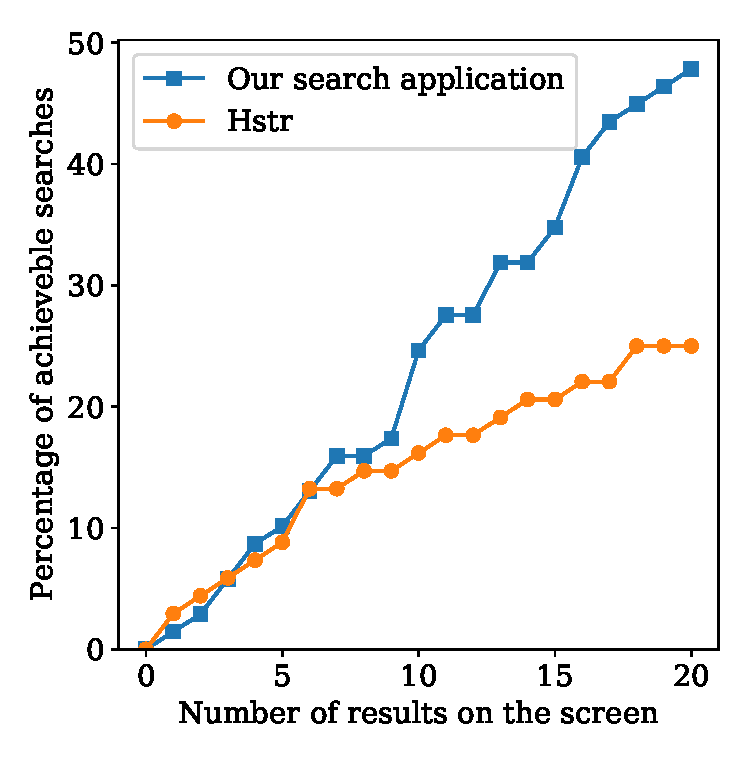
\includegraphics[width=0.5\linewidth]{figures/testing/testing-metrics-dist-0-cmds-resh.pdf}}
\caption{Achievable searches with zero knowledge (more is better)}
\small{Originally usage of Hstr (left) and usage of our search application (right)}
\label{eval-metrics-plot-dist-0-cmds}
\end{figure}

\begin{figure}
\centering
\tmpframe{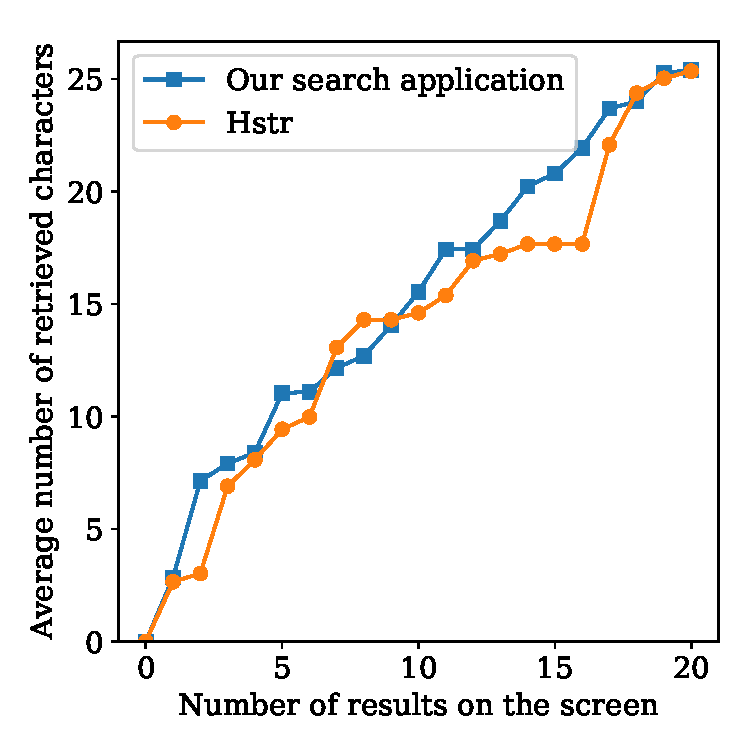
\includegraphics[width=0.5\linewidth]{figures/testing/testing-metrics-dist-0-chars-hstr.pdf}}\hfill
\tmpframe{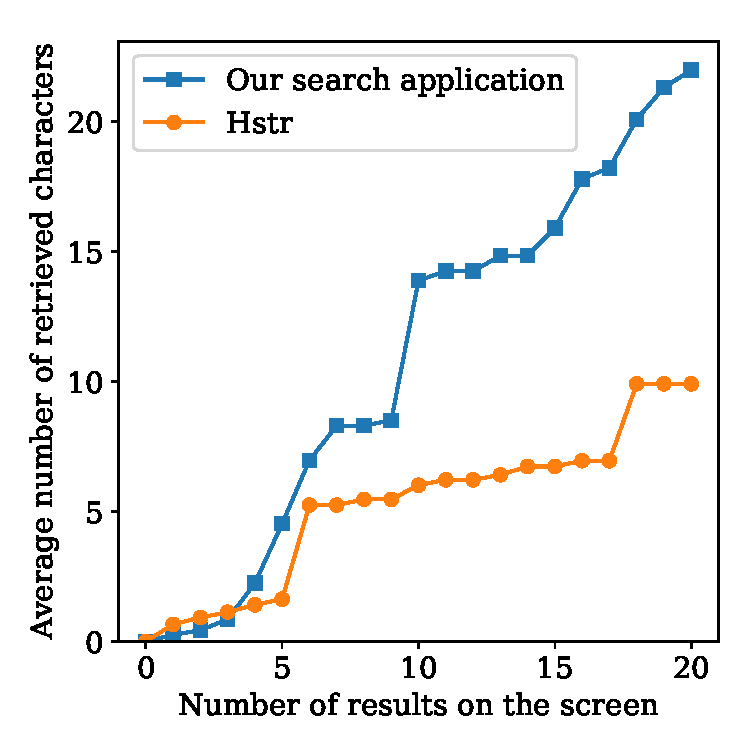
\includegraphics[width=0.5\linewidth]{figures/testing/testing-metrics-dist-0-chars-resh.pdf}}
\caption{Average saved characters with zero knowledge (more is better)}
\small{Originally usage of Hstr (left) and usage of our search application (right)}
\label{eval-metrics-plot-dist-0-chars}
\end{figure}


\newpage
\paragraph{Achievable searches with a single word query}

Once again, we are interested in finding out how many searches are achievable if we only look at a given number of top results. This time however, we provide a single knowledge token as a query to the search tools.

As shown by the right part of figure \ref{eval-metrics-plot-dist-1-cmds}, our search application can complete more searches than Hstr. Now that we provide a query to the searching tools the difference is less striking (compare figure \ref{eval-metrics-plot-dist-0-cmds} and \ref{eval-metrics-plot-dist-1-cmds}). We can see how even a single query word has a serious influence over the scoring function and by extension displayed results. 

Right part of \ref{eval-metrics-plot-dist-1-chars} shows a significant difference between Hstr and our solution. Hstr retrieves much shorter history entries than our search application. Our application saves considerably more typing to the user when a single word query is used. 

\subsection{Evaluating metrics}

We conclude that our history search application and Hstr perform similarly in all tasks that the user originally performed using Hstr. Contrarily, Hstr does not perform well in all situations when our application can be used. It appears that our solution covers extra workflows that are more difficult to achieve with Hstr. Examples of such workflows are described in previous section \ref{test-real-life-scenarios}. 
%It seems that users learn what their tools can or cannot do and use them accordingly.

Our search application enables users to retrieve history entries with less typing and remembering. Specifically, with no query, Hstr can only complete about half of the amount of searches our solution can. 

Furthermore, our search application on average retrieves longer history entries from history. Longer history entries take longer to type and remember. This means that the average effort saved to the user should be higher when using our solution. 

One thing we should point out is that we have used the same full shell history for both Hstr and our search application. Hstr normally uses standard shell history which might be missing some history entries. In reality, we expect the performance of Hstr to degrade because of the missing history entries.

% In all previous comparisons, Hstr might have performed differently. For example, we would expect degraded performance if many of the desired history entries were missing in the standard shell history.

\begin{figure}
\centering
\tmpframe{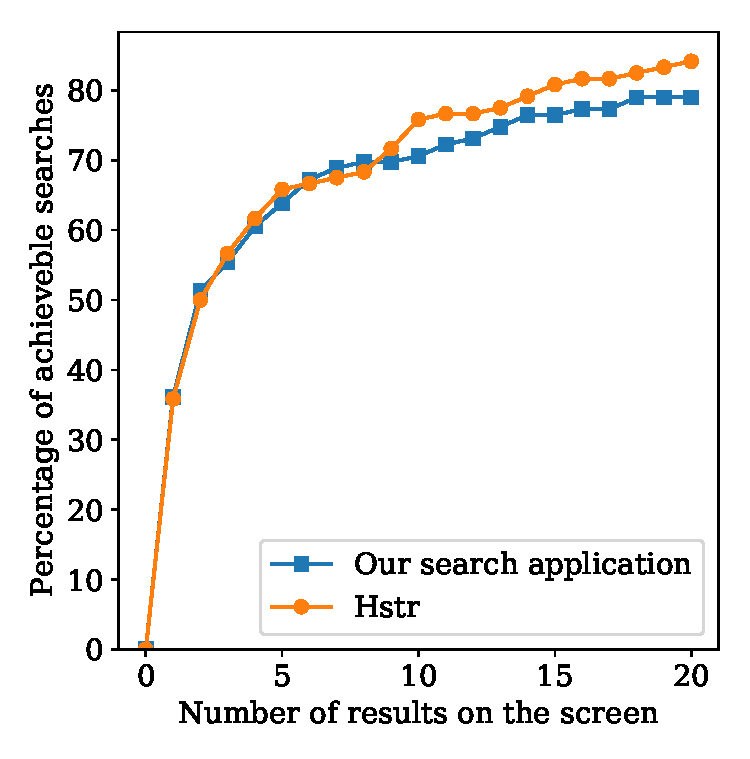
\includegraphics[width=0.5\linewidth]{figures/testing/testing-metrics-dist-1-cmds-hstr.pdf}}\hfill
\tmpframe{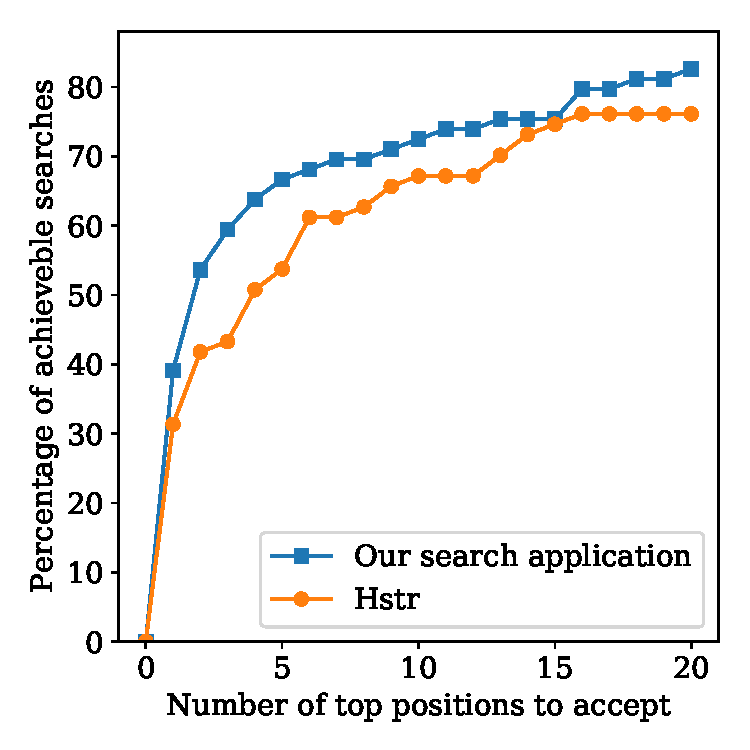
\includegraphics[width=0.5\linewidth]{figures/testing/testing-metrics-dist-1-cmds-resh.pdf}}
\caption{Achievable searches with a single knowledge token (more is better)}
\small{Originally usage of Hstr (left) and usage of our search application (right)}
\label{eval-metrics-plot-dist-1-cmds}
\end{figure}

\begin{figure}
\centering
\tmpframe{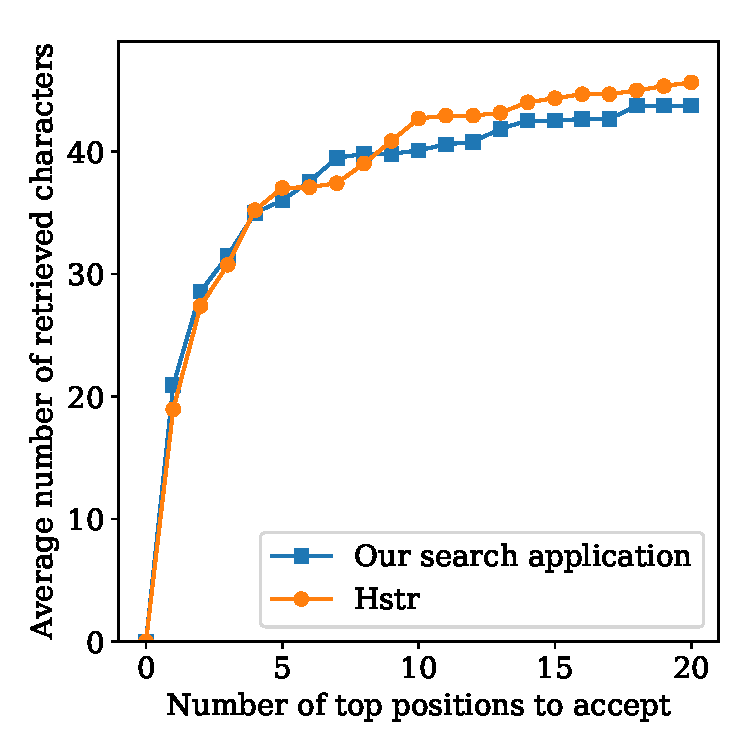
\includegraphics[width=0.5\linewidth]{figures/testing/testing-metrics-dist-1-chars-hstr.pdf}}\hfill
\tmpframe{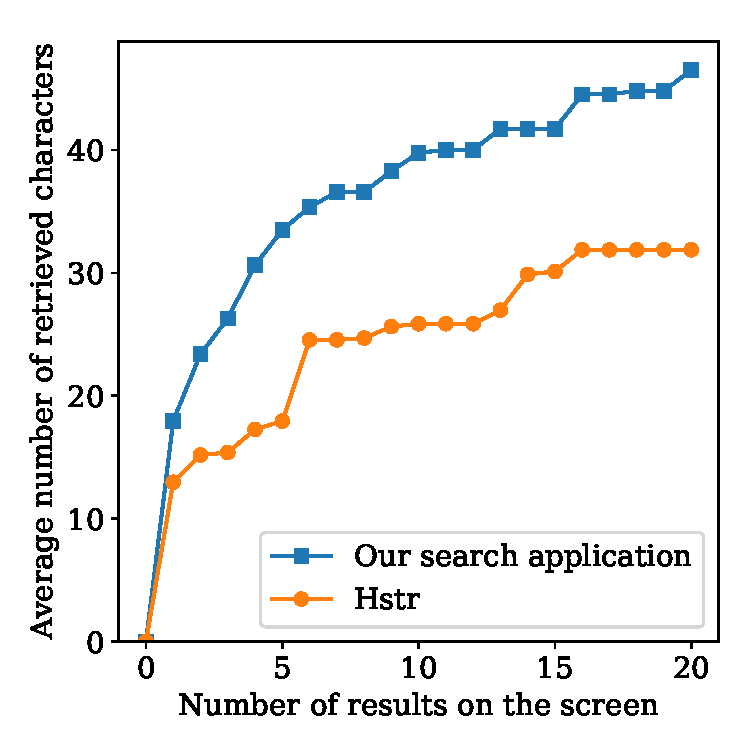
\includegraphics[width=0.5\linewidth]{figures/testing/testing-metrics-dist-1-chars-resh.pdf}}
\caption{Avg. saved chars. with a single knowledge token (more is better)}
\small{Originally usage of Hstr (left) and usage of our search application (right)}
\label{eval-metrics-plot-dist-1-chars}
\end{figure}

%\redtext{TODO: increase the size of the images if you manage shrink the captions}

\section{User feedback}

In this section, we describe how we released the project to the public, what improvements we made based on interviewing our users, and what feedback we get from users,

We released the first prototype of the search application about five months ago. We are engaging with the community and incrementally updating and improving the project. 

\subsection{User adoption}

Since the release of the first prototype of the search application four months ago the project was downloaded and installed over 600 times. 

The project also received over 250 stars on GitHub which is a bookmarking and endorsement feature on the GitHub website.\cite{github-stars}\cite{resh-github-homepage}

% https://keep.google.com/u/0/#NOTE/1pMiUTB0AU_JLmuiPByH7lHyzJR8_brmRqsiOeXRFez5t6wb0OUFtlinZ4oVNGpS9wRl_


\subsection{Feedback from the users}

Here, we describe what improvements we made to the project and what feedback we got from our users. We only mention a few examples of changes and feedback.

\paragraph{Non-contextual mode}

Some of the users were asking for a way to turn off the contextual search because it can occasionally get in their way. For example, logging into remote servers with \verb|ssh| can be done regardless of current directory. When searching for past \verb|ssh| commands the contextual search might do more harm than good.

Based on this we have added the ability to switch between contextual and non-contextual mode with \verb|CTRL-R|. This way the user can always choose the appropriate tool for the specific situation. Screenshot of the non-contextual mode is shown in figure \ref{xterm-resh-raw-80}.

\begin{figure}
\permanentframe{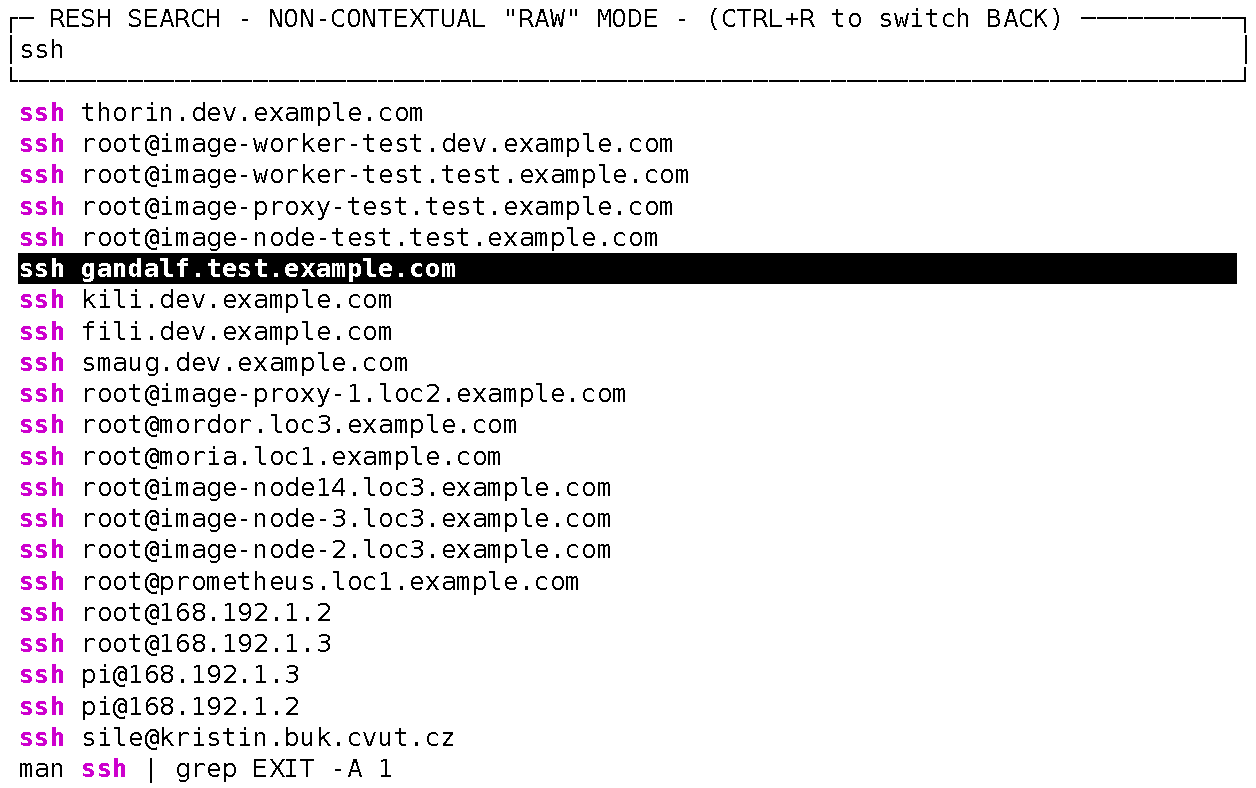
\includegraphics[width=0.995\linewidth]{figures/testing/xterm-resh-raw-80.pdf}}
\caption{Screenshot of the non-contextual mode of the search application}
\label{xterm-resh-raw-80}
\end{figure}

\paragraph{More ergonomic arrow key bindings}

One of our users was complaining that he is used to repeatedly pressing \verb|CTRL-R| to navigate to between the search results. He was previously using the standard reverse search.

By interviewing the user we discovered that he needs more ergonomic key bindings for arrow keys because they are quite far away from the home row. We have added alternative emacs-inspired bindings for arrow keys; Pressing \verb|CTRL-N| selects the next result on the page and \verb|CTRL-P| selects the previous one.   


\paragraph{Special handling for exit status}

We got some feedback regarding using exit status as part of contextual search. When users kill the running command using \verb|CTRL-C| it exits with the status of 130.
We anticipated that this would happen but it is more common than we expected.
We could add special handling for exit statuses that have special meaning. This feature, however, is not included in the current release.

%\redtext{SKIP ?}
%\begin{itemize}
%    \item Better help / onboarding
%    \item Directory jumping - history vs. specialised tools
%\end{itemize}


\subsection{User testimonies}

Now, we sum up what people say about the project. 

In our sizeable user base we have people who have switched from Hstr to our history system. Multiple people have said that our search application have fully replaced Hstr in their workflows. It seems that we provide a reasonable alternative to Hstr.

We shared the project online on multiple occasions and the feedback we received from people was overwhelmingly positive.\cite{resh-feedback}\cite{resh-feedback2}

\section{Additional workflows}

In this section, we describe additional workflows that are possible to complete using our search application. 

\subsection{Quickly retrieve history from other sessions}

Since standard history is handled individually in each session users cannot access history from other simultaneously running sessions. 

Our search applications uses history from all running sessions immediately. This means that user can quickly access history from another open terminals. 

Specifically, pressing \verb|CTRL-R| twice launches the search application and switches to non-contextual mode. This way the user can see all recent history entries from all sessions.

\subsection{Find similar history entries}

When the search application is launched, the contents of the command line are used as the initial query. For example, the user can use \verb|ARROW_UP| to retrieve the previous history entry and then press \verb|CTRL-R|. 

Using a full command line entry as a query fills the page with similar history entries. This is possible because of properties of our scoring function; It returns reasonable results even when there are words in the query that do not match anything. 

\subsection{Write new command line entries based on history}

Sometimes we want to write a new command line entry but we do not quite remember all of its parts. To make the writing easier it would be useful to see other similar history entries while we are constructing the new one.

As we already mentioned, when launching the search application the contents of the command line are used as a query. Conversely, the user can press \verb|CTRL-G| to abort the search and the contents of the query are pasted back onto the command line.
Combination of these two actions makes it possible to transfer back and forth between the command line and the search application. 

%All this can be used to write new command line entries while

We can launch the search application and start writing the command line entry into the query field. The search application continuously shows us similar history entries we can use as an inspiration. When we are done with typing the command line entry, we use \verb|CTRL-G| to get back to the command line. Then, we can execute the command line entry.


\section{Evaluation conclusion}

\redtext{Consider redoing this as paragraphs with bold first word}

Here, we sum up our findings from testing and evaluating our history searching solution. We point out why our search application is a useful replacement for both standard reverse search and Hstr. 

Our search application matches the usability improvements that Hstr offers compared to standard reverse search. We have shown this using chosen real life scenarios.

There are tasks that the observed user completed using Hstr. Our search application matches the searching performance of Hstr in all of those situations. This means that using our solution instead of Hstr does not lead to degraded performance.

There are new workflows that are easier to perform using our search application. Hstr does not perform well in those situations. Real life examples of such situations are described in section \ref{test-real-life-scenarios}.

Our solution can complete more searches with less knowledge and typing compared to Hstr. If the user switched back to Hstr, he would have to use queries in about half of all searches that are possible with zero knowledge in our search application. Our search application also retrieves longer history entries which saves more typing and remembering to the user.

The average performance of our search application is either comparable or better than Hstr depending on a specific situation. In many situations, however, our solution performs significantly better than Hstr. Because of that, we conclude that the contextual search is a great default way to search history. Furthermore, users have the option to switch between contextual and non-contextual mode. This is useful for retrieving history entries that are clearly non-contextual.
    
We released the first prototype of the search application about five months ago. Since then the application has grown in popularity and it was installed over 600 times. We have received overwhelmingly positive feedback. There are people who switched from Hstr to our search application and say that our solution has fully replaced all their Hstr workflows.





\begin{conclusion}

\redtext{Intro the problem, explain why we solved it and THEN describe how}



We have described shell history features available in current standard shells and pointed out their disadvantages. 
We have described the target users of our shell history tool. Based on shell history we collected, we have formulated typical workflows that accomplish different tasks using shell history. We have provided a detailed explanation of these workflows, pointing out issues with standard shell history mechanisms. As the main finding, we have identified reverse search as a very inefficient history feature that is worth redesigning.

We have explored what popular history tools are available. We have found state-of-the-art non-contextual history tools that provide a major improvement over standard history by replacing reverse search. These tools address the specific issues of reverse search we identified. We found contextual history tools that are based on appealing ideas; These tools, however, do not match the improvements provided by state-of-the-art non-contextual history tools. We have described how available contextual information relates to the ways people use shell. \redtext{TODO: shorten analysis above as necessary}


% design

Based on our previous analysis, we have designed a history system. The design is a result of the iterative process that involved feedback from users. Our design matches the improvements of the state-of-the-art non-contextual history tools. Furthermore, it uses context to enhance the capabilities of the shell history. The design was tested to make sure that it fulfills all set requirements. 

% implementation

We have implemented a significant portion of the design. The working solution records shell history with context and usage. It features a fullscreen terminal application that searches shell history and shows relevant results based on the current context. Without any search query, the application offers history entries from the current context. 

% evaluation/testing


We have evaluated the performance of the search application and compared it with both state-of-the-art history tool and standard builtin history search feature. 
We have suggested metrics and used them to compare our solution with state-of-the-art history searching tool -- Hstr \cite{toolshstr}.
The average performance of our history searching application is either similar or better than Hstr. 

We have found real-life situations where our solution provides a significant advantage over both standard reverse search and Hstr.
Our solution enables the user to search with significantly less knowledge and typing. Furthermore, our search application, on average, saves more typed characters to the user. 
We have concluded that contextual search is a great default because it offers new possibilities without degrading the average performance.


As a result of feedback from our users, we have added several features to the search application. Notably, users can switch between default contextual search and non-contextual search. This is great for specific situations where using context does not bring value.

Since the release of the first prototype, the search application has been installed over 600 times. The project has over 250 stars on GitHub. The feedback we have received is overwhelmingly positive. %We have also got a chance to present one of the first versions of the application on Installfest conference. \cite{installfest-talk}\cite{installfest} 

Right now, we want to encourage you, the reader, to try out the project for yourself. You can find installation instructions on the GitHub page of the project: \url{https://github.com/curusarn/resh} %\cite{resh-github-homepage}


\paragraph{Future work}

Our work implements the core functionality of the designed history system. However, the remaining parts of the design should also be implemented because they provide considerable value to the users.

One part of the design we want to point out is synchronization.
Implementing the synchronization connectors for the daemon would enable history searching across devices. It would also make the stored history replicated, which could prevent potential data loss.

Outside of the things we have included in the design, we suggest an improvement for our search application based on existing research. According to \cite{greenberg1993computer}, history entries that were already retrieved should be easier to retrieve in the future. The scoring function should be modified to include this extra factor. 

Additionally, we propose a topic for future research. Using machine learning techniques and context to provide Autosuggestions tailored to the user is a promising topic for a thesis. 

More research should be done to explore relationships between history entries. Exploring how terminal sessions and sequences of history entries relate to workflows of people could bring useful insights. These insights could be used to improve history searching tools.

\end{conclusion}

\bibliographystyle{iso690.bst}
\bibliography{ref}

\appendix

%\printglossaries

\chapter{Contents of attached medium}\label{app:SDcontent}

\todotext{TODO: Visualise the contents of enclosed media. Use of dirtree is recommended. Note that directories src and text with appropriate contents are mandatory.}


\begin{figure}
	\dirtree{%
		.1 readme.txt\DTcomment{the file with CD contents description}.
		.1 data\DTcomment{the data files directory}.
		.2 graphs\DTcomment{the directory of graphs of experiments}.
		.3 *.eps\DTcomment{the B/W graphs}.
		.3 *.png\DTcomment{the color graphs}.
		.3 *.dat\DTcomment{the graphs data files}.
		.1 exe\DTcomment{the directory with executable WBDCM program}.
		.2 wbdcm\DTcomment{the WBDCM program executable (UNIX)}.
		.2 wbdcm.exe\DTcomment{the WBDCM program executable (Windows)}.
		.1 src\DTcomment{the directory of source codes}.
		.2 wbdcm\DTcomment{the directory of WBDCM program}.
		.3 Makefile\DTcomment{the makefile of WBDCM program (UNIX)}.
		.2 thesis\DTcomment{the directory of \LaTeX{} source codes of the thesis}.
		.3 figures\DTcomment{the thesis figures directory}.
		.3 *.tex\DTcomment{the \LaTeX{} source code files of the thesis}.
		.1 text\DTcomment{the thesis text directory}.
		.2 thesis.pdf\DTcomment{the Diploma thesis in PDF format}.
		.2 thesis.ps\DTcomment{the Diploma thesis in PS format}.
	}
\end{figure}

\chapter{Additional notes}\label{app:extras}

\redtext{This should not be empty}

\newpage
\section{Sequential structure of command usage}\label{seq-app}

Figure \ref{seq-graph} shows sequential relationships between command stubs in shell usage of a single chosen user. 

The graph contains 41 most used commands. Each node represents a command stub, and its size is proportionate to the command stub frequency. Each vertex represents a transition probability from one command to the next one. Nodes \verb|_start_| and \verb|_end_| represent the beginning and end of terminal sessions.

We can see that there are significant dependencies between command stubs. Many commands repeat themselves with high probabilities. There are also high probability transitions between specific commands. For example, \verb|mkdir| is followed by \verb|cd| in 90\% of situations.

%This is all interesting, but is it usable in practice? Do people even recognize these sequential relationships in their shell usage?
We created sequential graphs like this based on the shell history of different users. When we show these graphs to the original user, they always instantly recognize their history. Furthermore, they can immediately spot and describe the workflows different sequences in the graph represent.

\begin{figure}

\tmpframe{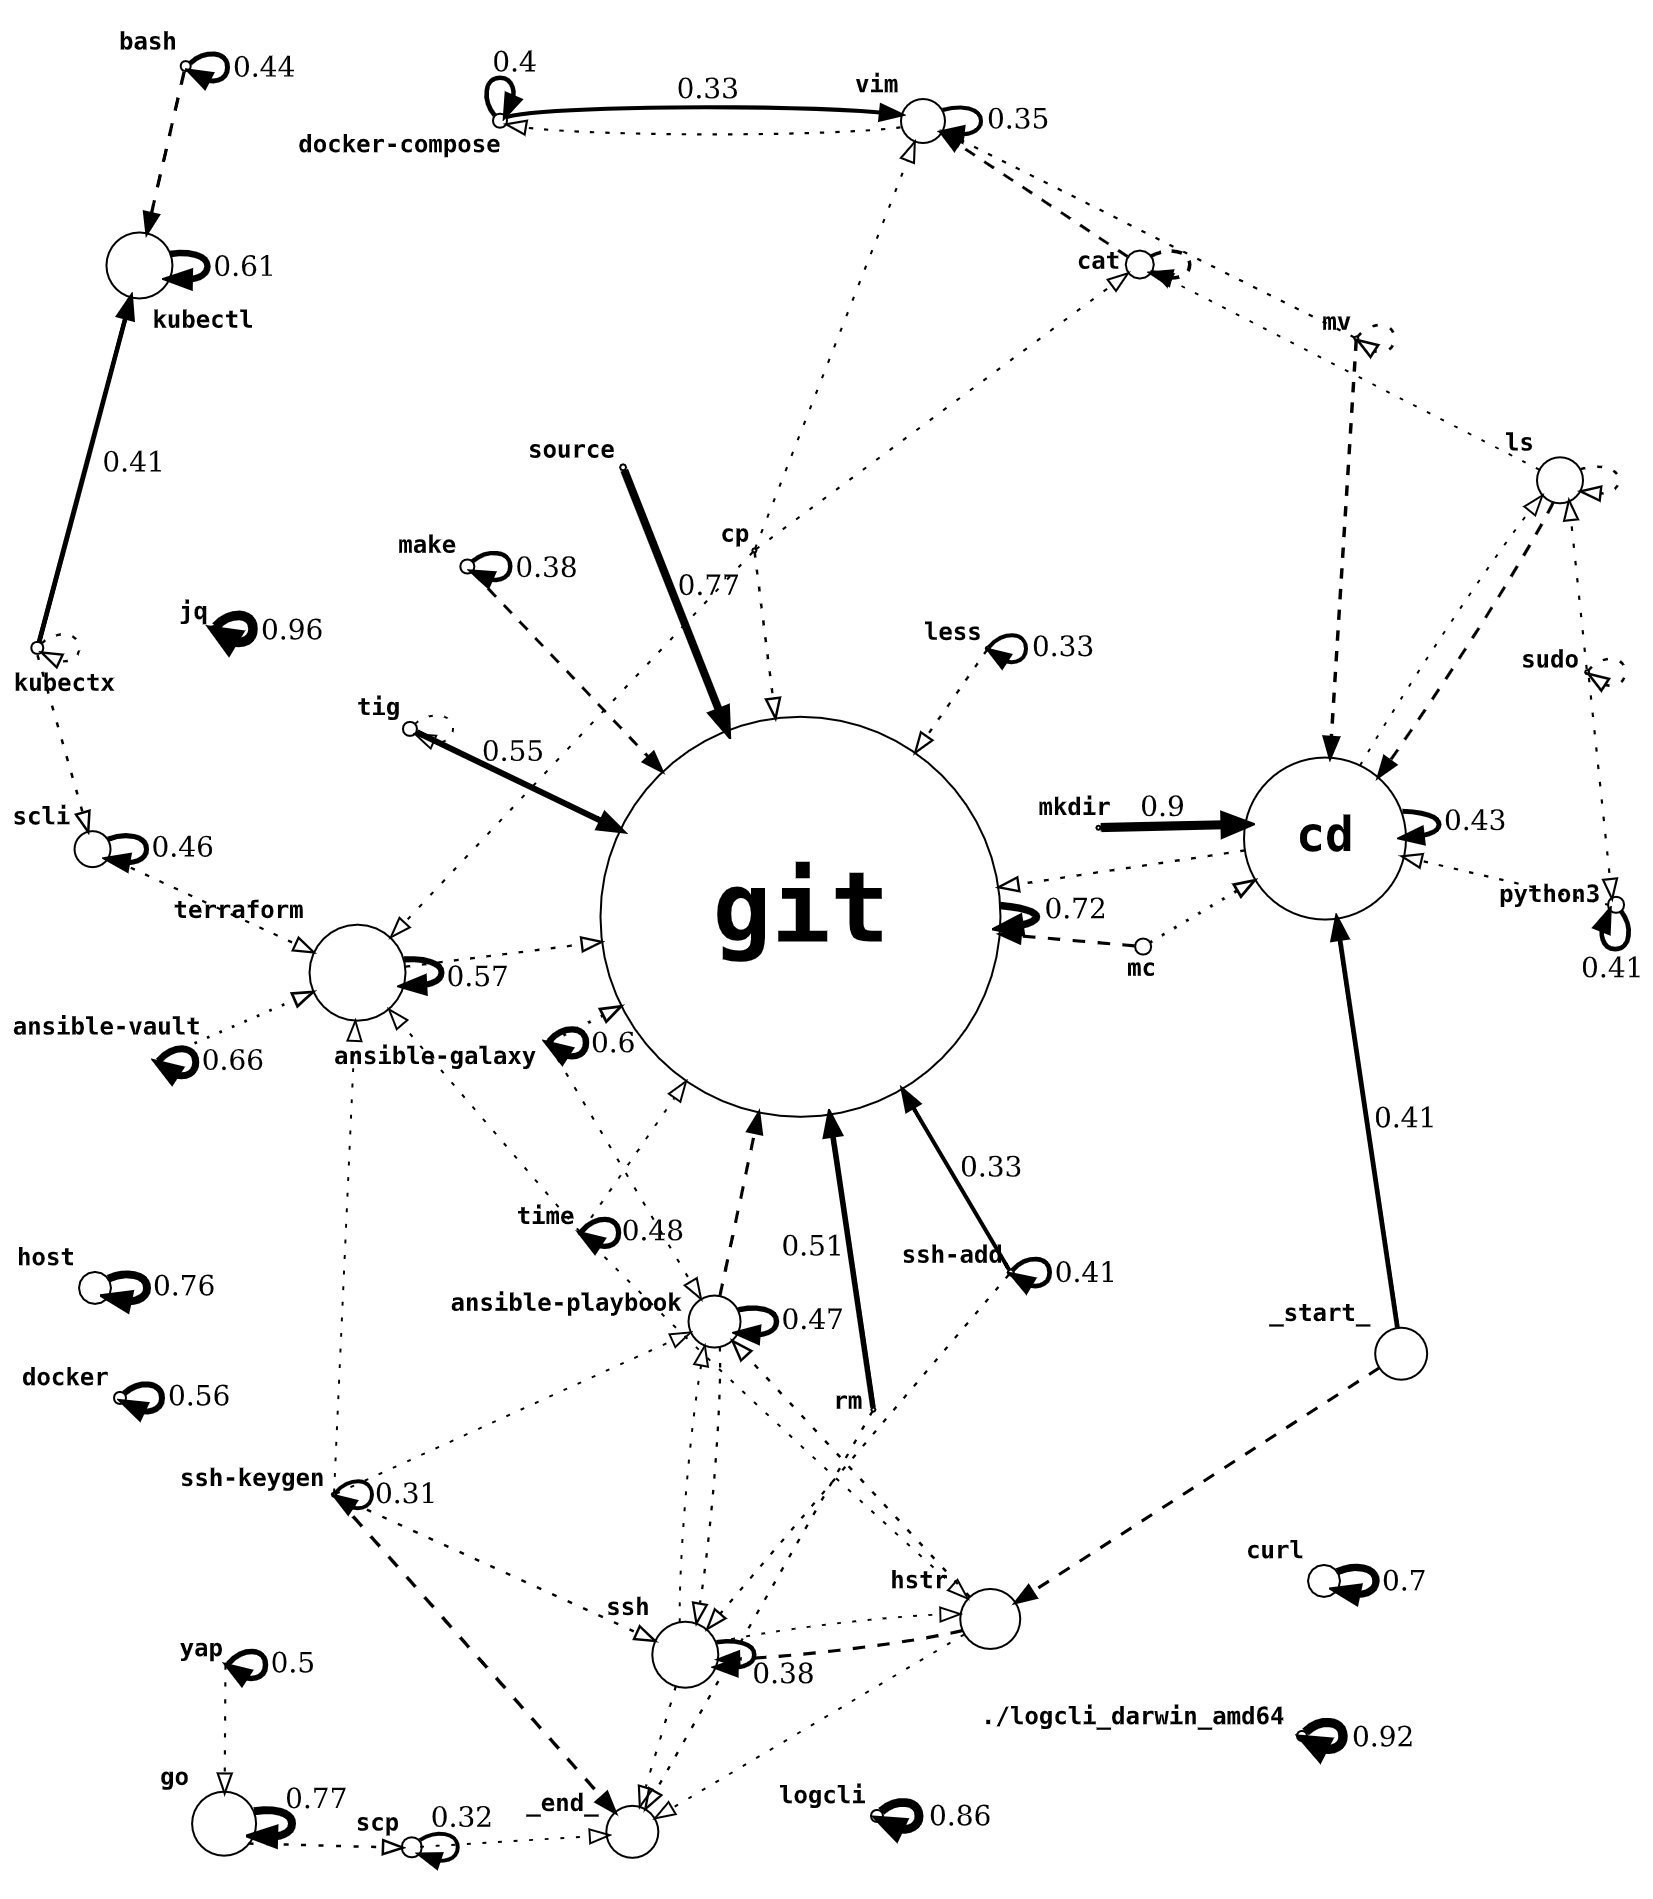
\includegraphics[width=\linewidth]{figures/greenberg_new/graph_cmd-sequence_vit_41_0-1_crop.png}}
%\newline
%\newline
\centering
\begin{tabular}{|l|l|}
\hline
Vertex style & Transition probability            \\\hline
Regular/full     & 1.0 -- 0.3 (specified by labels) \\
Dashed      & 0.3 -- 0.2                         \\
Dotted      & 0.2 -- 0.1                         \\
\hline
\end{tabular}
%\caption{Sequential structure of command usage (legend).}
%\label{tab:seq-table}

\caption{Sequential structure of command usage.}
\label{seq-graph}
\end{figure}



\end{document}
